\documentclass[plainsections,alongposter]{sciposterlocal}

\usepackage{multicol}
\usepackage{mathpazo} % Better fonts
\usepackage{parskip}
\usepackage{amsmath}
\usepackage{booktabs}
\usepackage[utf8]{inputenc}
\usepackage{graphicx}
\usepackage[np]{numprint}
\usepackage{tikz}
\usepackage{gnuplot-lua-tikz}
%\usepackage{lineno}
%\linenumbers

%
% Macros
%
\newcommand{\tr}{\rm{Tr}}
\newcommand{\mean}[1]{\left\langle{#1}\right\rangle}
\newcommand{\comment}[1]{{\bf\textit{#1}}}

%%%%%%%%%%%% Header info
\title{The QCD phase-diagram obtained from the NJL and the extended-NJL models for quark and hadron phases}

\author{Clebson A. Graeff$^\dagger$; Débora P. Menezes$^*$}
\email{cgraeff@utfpr.edu.br, debora.p.m@ufsc.br}

\institute{$^\dagger$~Universidade Tecnológica Federal do Paraná -- Pato Branco, PR - Brazil \\
$^*$~Universidade Federal de Santa Catarina -- Florian\'opolis, SC - Brazil \\
}

\leftlogo{Logo_UTFPR_PB_cor.pdf}
\rightlogo{Brasao_UFSC_PDF.pdf}
%%%%%%%%%%%%

%%% Color for sections titles
\definecolor{SectionColor}{rgb}{0.22,0.33,0.6}

%%% Set roman fonts instead of sans serif
\renewcommand{\familydefault}{\rmdefault}

%%% No rules between columns, please
\setlength{\columnseprule}{0pt}

%%% BibTeX bibliography style
\bibliographystyle{plain}

%%%%%%%%%%%%%%%%%%%%
%%% The Document %%%
%%%%%%%%%%%%%%%%%%%%
\begin{document}

\maketitle % The Header

\begin{multicols}{2} % Start content area

%%%%%%%%%%%%%%%%%%%
\section*{Abstract}
{ \it
We analyse the hadron/quark phase transition described by the Nambu-Jona-Lasinio (NJL) model [quark phase] and the extended Nambu-Jona-Lasinio model (eNJL) [hadron phase]. While the original formulation of NJL model is not capable of describing hadronic properties due to its lack of confinement, it can be extended with a scalar-vector interaction so it exhibits this property, the so-called  eNJL model. As part of this analysis, we obtain the equations of state within the SU(2) versions of both models for the hadron and the quark phases and determine the binodal surface. 
}

%%%%%%%%%%%%%%%%%%%%%%%
\section*{Motivation}

The study of the QCD phase-diagram, is relevant to the understanding of many aspects of the physics in our universe. Two of the aspects of interest are related to relativistic heavy ion collisions (low densities, high temperatures) and stars (high densities, low temperatures). However, the direct solution of QCD is not possible at finite chemical potential.

Given the importance of the study of the phases and the phase separation boundaries, we propose an investigation of the hadron/quark phase transition within a two phase model.

%%%%%%%%%%%%%%%%%%%%%%%%%%%%%
\section*{Quark phase matter}

The quark phase is described by a SU(2) NJL model lagrangian, including a vector-isoscalar term, given by \cite{Buballa2005}
\begin{equation}\label{Eq:LagNJL-SU2-Bub}
	\mathcal{L} =\bar{\psi}(i\gamma^\mu\partial_\mu - m_0)\psi + G_S[(\bar{\psi}\psi)^2 + (\bar{\psi}i\gamma_5\vec{\tau}\psi)^2] - G_V(\bar{\psi}\gamma^\mu \psi)^2.
\end{equation}
%
Here $\psi$ represents the quark field, $m_0$ the quark bare mass, and $G_S$ and $G_V$ are coupling constants that are chosen by fitting the pion mass $m_\pi = \np[MeV]{135.0}$ and decay constant $f_\pi = \np[MeV]{92.4}$. As the theory is non-renormalizable, a momentum cutoff $\Lambda$ is employed, which acts as a new parameter.

\begin{table}
\centering
\caption{Parameters sets for the lagrangian density~\eqref{Eq:LagNJL-SU2-Bub} \cite{Buballa1996, Buballa2005}. \label{Tab:Parametros_NJL}}
\begin{tabular}{lcccccccc}
\toprule
Model &  $\Lambda$ & $G_S$ ($\rm{fm}^2$) & $G_V$ ($\rm{fm}^2$) & $m_0$ (MeV) & $m$ (MeV) \\
\midrule
Buballa-1 & 650 & 0.19721 & -- & 0 & 313 \\
Buballa-2 & 600 & 0.26498 & -- & 0 & 400 \\
Buballa-3 & 570 & 0.34034 & -- & 0 & 500 \\
%BuballaR-1 & 664.3 & 0.18176 & $\propto G_S$ & 5.0 & 300 \\
BuballaR-2 & 587.9 & 0.27449 & 0 & 5.6 & 400 \\
BuballaR-2$_{G_V}$ & 587.9 & 0.27449 & $G_V = G_S$ & 5.6 & 400\\
%BuballaR-3 & 569.3 & 0.33759 & $\propto G_S$ & 5.5 & 500 \\
%BuballaR-4 & 568.6 & 0.38178 & $\propto G_S$ & 5.1 & 600
\bottomrule
\end{tabular}
\end{table}

%%%%%%%%%%%%%%%%%%%%%%%%%%%%%%
\section*{Hadron phase matter}

Even though the original NJL model is unable to describe the saturation properties of the nuclear matter, this can be fixed by the inclusion of extra channels which combine the scalar and vector terms~\cite{Koch1987}. An extended NJL model (eNJL)~\cite{Pais2016} which includes such channel is given by the lagrangian density
\begin{equation}\label{Eq:Lagrangiana_eNLJ_Pais}
\begin{split}
	\mathcal{L} =&~ \bar{\psi}(i\gamma^\mu\partial_\mu - m_0)\psi + G_s[(\bar{\psi}\psi)^2 + (\bar{\psi}i\gamma_5\vec{\tau}\psi)^2] - G_v(\bar{\psi}\gamma^\mu\psi)^2 \\
	& - G_{sv}[(\bar{\psi}\psi)^2 + (\bar{\psi}i\gamma_5\vec{\tau}\psi)^2](\bar{\psi}\gamma^\mu\psi)^2 \\
	& - G_\rho[(\bar{\psi}\gamma^\mu\vec{\tau}\psi)^2 + (\bar{\psi}\gamma_5\gamma^\mu\vec{\tau}\psi)^2] \\
	& - G_{v\rho}(\bar{\psi}\gamma^\mu\psi)^2[(\bar{\psi}\gamma^\mu\vec{\tau}\psi)^2 + (\bar{\psi}\gamma_5\gamma^\mu\vec{\tau}\psi)^2] \\
	& - G_{s\rho} [(\bar{\psi}\psi)^2 + (\bar{\psi}i\gamma_5\vec{\tau}\psi)^2][(\bar{\psi}\gamma^\mu\vec{\tau}\psi)^2 + (\bar{\psi}\gamma_5\gamma^\mu\vec{\tau}\psi)^2].
\end{split}
\end{equation}
%
where $\psi$ represents the nucleon field and the constants $G_i$ represents the coupling constants for the different channels.

\begin{table}
\centering
\caption{Parameters sets for the lagrangian density~\eqref{Eq:Lagrangiana_eNLJ_Pais} \cite{Pais2016}. \label{Tab:Parametros_eNJL}}
\begin{tabular}{lcccccccc}
\toprule
Model & $G_s$ ($\rm{fm}^2$) & $G_v$ ($\rm{fm}^2$) & $G_{sv}$ ($\rm{fm}^8$) & $G_\rho$ ($\rm{fm}^2$) & $G_{v\rho}$ ($\rm{fm}^8$) & $G_{s\rho}$ ($\rm{fm}^8$) & $\Lambda$ (MeV) & $m$ (MeV) \\
\midrule
eNJL1 & 4.855 & 4.65 & -6.583 & 0.5876 & 0 & 0 & 388.189 & 0 \\
eNJL1$\omega\rho$1 & 4.855 & 4.65 & -6.583 & 0.5976 & -1 & 0 & 388.189 & 0 \\
%eNJL1$\omega\rho$2 & 4.855 & 4.65 & -6.583 & 0.6476 & -6 & 0 & 388.189 & 0 \\
eNJL2 & 3.8 & 3.8 & -4.228 & 0.6313 & 0 & 0 & 422.384 & 0 \\
eNJL2$\omega\rho$1 & 3.8 & 3.8 & -4.228 & 0.6413 & -1 & 0 & 422.384 & 0 \\
eNJL3 & 1.93 & 3.0 & -1.8 & 0.65 & 0 & 0 & 534.815 & 0 \\
eNJL3$\sigma\rho$1 & 1.93 & 3.0 & -1.8 & 0.0269 & 0 & 0.5 & 534.815 & 0 \\
eNJL1m & 1.3833 & 1.781 & -2.943 & 0.7 & 0 & 0 & 478.248 & 450 \\
%eNJL1m$\sigma\rho$1 & 1.3833 & 1.781 & -2.943 & 0.0739 & 0 & 1 & 478.248 & 450 \\
eNJL2m & 1.078 & 1.955 & -2.74 & 0.75 & 0 & 0 & 502.466 & 450 \\
%eNJL2m$\sigma\rho$1 & 1.078 & 1.955 & -2.74 & -0.1114 & 0 & 1 & 502.466 & 450 \\
\bottomrule
\end{tabular}
\end{table}

%%%%%%%%%%%%
\columnbreak

%%%%%%%%%%%%%%%%%%%
\section*{Binodals}

The phase coexistence may be determined using the Gibbs' conditions \cite{Cavagnoli2011}:

\begin{minipage}{0.5\columnwidth}
\begin{align*}
\mu_B^Q &= \mu_B^H\\
T^Q &= T^H \\
P^Q &= P^H
\end{align*}
\end{minipage}
\begin{minipage}{0.5\columnwidth}
\begin{align*}
	\mu_B^H &= \frac{\mu_p + \mu_n}{2} \\
	\mu_B^Q &= \frac{3}{2} (\mu_u + \mu_d) = 3 \mu_q.
\end{align*}
\end{minipage}

\noindent{}where the indexes $H$ and $Q$ refer to the hadrons and quarks phases. The phase coexistence may then be obtained by simply plotting $P^i \times \mu_B^i$, $i = Q, H$, and looking for the intersection of both lines.

%%%%%%%%%%%%%%%%%%%%
\section*{Results}

We determine the equations of state for both models at $T = 0$ and proton fraction $y_p = \np{0.5}$ (code available at \texttt{github.com/cgraeff}). The realized phase of the system is the one which maximizes the pressure. This means that the crossing of the lines, as in Figure~\ref{Fig:Pressure_func_chemical_pot}, indicates a phase transition.

In Table~\ref{Tab:Transition_chemical_pot} we show the chemical potential $\mu_B^i$ at phase-transition for cominations of parameterizations of Tables~\ref{Tab:Parametros_NJL} and~\ref{Tab:Parametros_eNJL}. Combinations for which there is no transition are ommited.

\begin{figure}
\caption{Pressure as function of barionic chemical potential. The crossing point is the phase-coexistence point. Red curves represent hadrons, blue represent quarks. From left to right (quarks, hadrons): Buballa-1--eNJL3, Buballa-1--eNJL1$\omega\rho$1, BuballaR-2--eNJL2$\omega\rho$1.\label{Fig:Pressure_func_chemical_pot}}
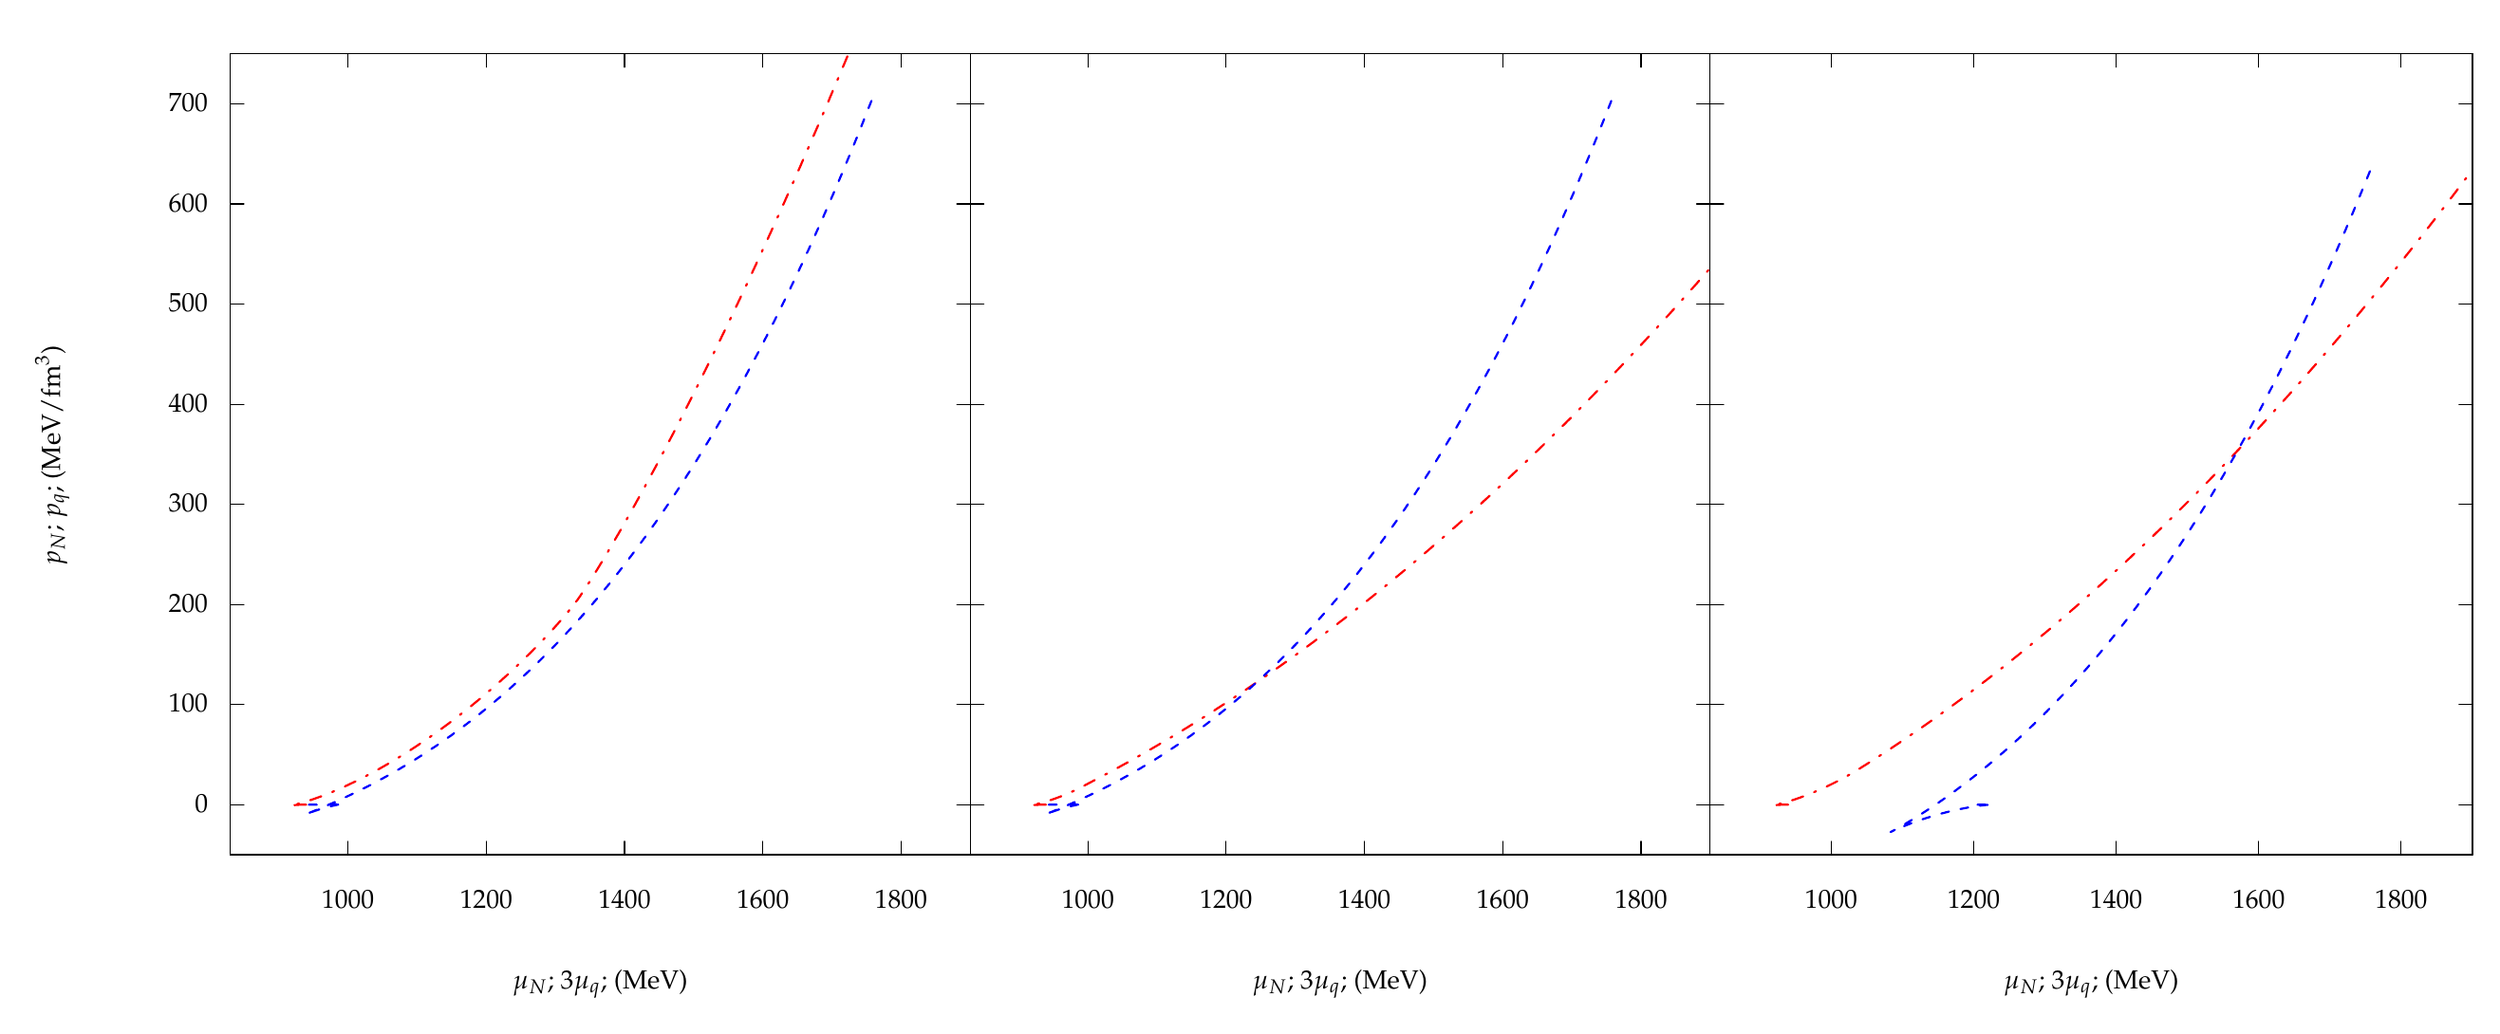
\begin{tikzpicture}[gnuplot]
%% generated with GNUPLOT 5.0p5 (Lua 5.3; terminal rev. 99, script rev. 100)
%% seg 28 nov 2016 20:16:52 BRST
\path (0.000,0.000) rectangle (30.000,13.000);
\gpcolor{color=gp lt color border}
\gpsetlinetype{gp lt border}
\gpsetdashtype{gp dt solid}
\gpsetlinewidth{1.00}
\draw[gp path] (0.000,2.579)--(0.180,2.579);
\draw[gp path] (9.899,2.579)--(9.719,2.579);
\node[gp node right] at (-0.184,2.579) {$0$};
\draw[gp path] (0.000,3.919)--(0.180,3.919);
\draw[gp path] (9.899,3.919)--(9.719,3.919);
\node[gp node right] at (-0.184,3.919) {$100$};
\draw[gp path] (0.000,5.260)--(0.180,5.260);
\draw[gp path] (9.899,5.260)--(9.719,5.260);
\node[gp node right] at (-0.184,5.260) {$200$};
\draw[gp path] (0.000,6.600)--(0.180,6.600);
\draw[gp path] (9.899,6.600)--(9.719,6.600);
\node[gp node right] at (-0.184,6.600) {$300$};
\draw[gp path] (0.000,7.940)--(0.180,7.940);
\draw[gp path] (9.899,7.940)--(9.719,7.940);
\node[gp node right] at (-0.184,7.940) {$400$};
\draw[gp path] (0.000,9.280)--(0.180,9.280);
\draw[gp path] (9.899,9.280)--(9.719,9.280);
\node[gp node right] at (-0.184,9.280) {$500$};
\draw[gp path] (0.000,10.621)--(0.180,10.621);
\draw[gp path] (9.899,10.621)--(9.719,10.621);
\node[gp node right] at (-0.184,10.621) {$600$};
\draw[gp path] (0.000,11.961)--(0.180,11.961);
\draw[gp path] (9.899,11.961)--(9.719,11.961);
\node[gp node right] at (-0.184,11.961) {$700$};
\draw[gp path] (1.573,1.909)--(1.573,2.089);
\draw[gp path] (1.573,12.631)--(1.573,12.451);
\node[gp node center] at (1.573,1.293) {$1000$};
\draw[gp path] (3.423,1.909)--(3.423,2.089);
\draw[gp path] (3.423,12.631)--(3.423,12.451);
\node[gp node center] at (3.423,1.293) {$1200$};
\draw[gp path] (5.273,1.909)--(5.273,2.089);
\draw[gp path] (5.273,12.631)--(5.273,12.451);
\node[gp node center] at (5.273,1.293) {$1400$};
\draw[gp path] (7.124,1.909)--(7.124,2.089);
\draw[gp path] (7.124,12.631)--(7.124,12.451);
\node[gp node center] at (7.124,1.293) {$1600$};
\draw[gp path] (8.974,1.909)--(8.974,2.089);
\draw[gp path] (8.974,12.631)--(8.974,12.451);
\node[gp node center] at (8.974,1.293) {$1800$};
\draw[gp path] (0.000,12.631)--(0.000,1.909)--(9.899,1.909)--(9.899,12.631)--cycle;
\node[gp node center,rotate=-270] at (-2.362,7.270) {$p_N$; $p_q$; ($\rm{MeV}/\rm{fm}^3$)};
\node[gp node center] at (4.949,0.215) {$\mu_N$; $3\mu_q$; (MeV)};
\gpcolor{rgb color={1.000,0.000,0.000}}
\gpsetdashtype{gp dt 6}
\gpsetlinewidth{2.00}
\draw[gp path] (1.012,2.579)--(1.011,2.579)--(1.010,2.579)--(1.009,2.579)--(1.007,2.579)%
  --(1.005,2.579)--(1.004,2.579)--(1.002,2.579)--(1.000,2.579)--(0.998,2.579)--(0.996,2.579)%
  --(0.993,2.579)--(0.991,2.579)--(0.989,2.579)--(0.987,2.579)--(0.985,2.579)--(0.982,2.579)%
  --(0.980,2.579)--(0.978,2.579)--(0.976,2.579)--(0.973,2.579)--(0.971,2.579)--(0.969,2.579)%
  --(0.966,2.578)--(0.964,2.578)--(0.962,2.578)--(0.960,2.578)--(0.957,2.578)--(0.955,2.578)%
  --(0.953,2.578)--(0.951,2.578)--(0.948,2.578)--(0.946,2.578)--(0.944,2.578)--(0.942,2.578)%
  --(0.939,2.578)--(0.937,2.578)--(0.935,2.577)--(0.933,2.577)--(0.931,2.577)--(0.929,2.577)%
  --(0.926,2.577)--(0.924,2.577)--(0.922,2.577)--(0.920,2.577)--(0.918,2.577)--(0.916,2.577)%
  --(0.914,2.577)--(0.912,2.576)--(0.910,2.576)--(0.908,2.576)--(0.906,2.576)--(0.904,2.576)%
  --(0.902,2.576)--(0.900,2.576)--(0.898,2.576)--(0.896,2.576)--(0.894,2.576)--(0.893,2.575)%
  --(0.891,2.575)--(0.889,2.575)--(0.887,2.575)--(0.885,2.575)--(0.884,2.575)--(0.882,2.575)%
  --(0.880,2.575)--(0.878,2.575)--(0.877,2.574)--(0.875,2.574)--(0.873,2.574)--(0.872,2.574)%
  --(0.870,2.574)--(0.868,2.574)--(0.867,2.574)--(0.865,2.574)--(0.864,2.574)--(0.862,2.573)%
  --(0.861,2.573)--(0.859,2.573)--(0.858,2.573)--(0.856,2.573)--(0.855,2.573)--(0.853,2.573)%
  --(0.852,2.573)--(0.851,2.572)--(0.849,2.572)--(0.848,2.572)--(0.847,2.572)--(0.845,2.572)%
  --(0.844,2.572)--(0.843,2.572)--(0.841,2.572)--(0.840,2.572)--(0.839,2.571)--(0.838,2.571)%
  --(0.837,2.571)--(0.835,2.571)--(0.834,2.571)--(0.833,2.571)--(0.832,2.571)--(0.831,2.571)%
  --(0.830,2.571)--(0.829,2.570)--(0.828,2.570)--(0.827,2.570)--(0.826,2.570)--(0.825,2.570)%
  --(0.824,2.570)--(0.823,2.570)--(0.822,2.570)--(0.821,2.570)--(0.820,2.570)--(0.819,2.569)%
  --(0.818,2.569)--(0.817,2.569)--(0.816,2.569)--(0.815,2.569)--(0.814,2.569)--(0.813,2.569)%
  --(0.812,2.569)--(0.811,2.569)--(0.811,2.568)--(0.810,2.568)--(0.809,2.568)--(0.808,2.568)%
  --(0.807,2.568)--(0.806,2.568)--(0.805,2.568)--(0.804,2.568)--(0.803,2.568)--(0.803,2.567)%
  --(0.802,2.567)--(0.801,2.567)--(0.802,2.567)--(0.803,2.567)--(0.803,2.568)--(0.804,2.568)%
  --(0.805,2.568)--(0.806,2.568)--(0.807,2.568)--(0.808,2.568)--(0.809,2.568)--(0.809,2.569)%
  --(0.810,2.569)--(0.811,2.569)--(0.812,2.569)--(0.813,2.569)--(0.814,2.570)--(0.815,2.570)%
  --(0.816,2.570)--(0.817,2.570)--(0.818,2.570)--(0.819,2.570)--(0.820,2.571)--(0.821,2.571)%
  --(0.822,2.571)--(0.823,2.571)--(0.824,2.572)--(0.825,2.572)--(0.826,2.572)--(0.827,2.572)%
  --(0.828,2.572)--(0.829,2.572)--(0.830,2.573)--(0.831,2.573)--(0.832,2.573)--(0.833,2.573)%
  --(0.834,2.574)--(0.835,2.574)--(0.836,2.574)--(0.837,2.574)--(0.838,2.574)--(0.839,2.575)%
  --(0.841,2.575)--(0.842,2.575)--(0.843,2.575)--(0.844,2.576)--(0.845,2.576)--(0.847,2.576)%
  --(0.848,2.577)--(0.849,2.577)--(0.850,2.577)--(0.852,2.577)--(0.853,2.578)--(0.854,2.578)%
  --(0.856,2.578)--(0.857,2.579)--(0.858,2.579)--(0.860,2.579)--(0.861,2.580)--(0.862,2.580)%
  --(0.864,2.580)--(0.865,2.581)--(0.867,2.581)--(0.868,2.581)--(0.870,2.582)--(0.871,2.582)%
  --(0.873,2.582)--(0.874,2.583)--(0.876,2.583)--(0.877,2.584)--(0.879,2.584)--(0.881,2.584)%
  --(0.882,2.585)--(0.884,2.585)--(0.885,2.586)--(0.887,2.586)--(0.889,2.586)--(0.891,2.587)%
  --(0.892,2.587)--(0.894,2.588)--(0.896,2.588)--(0.897,2.589)--(0.899,2.589)--(0.901,2.589)%
  --(0.903,2.590)--(0.905,2.590)--(0.906,2.591)--(0.908,2.591)--(0.910,2.592)--(0.912,2.592)%
  --(0.914,2.593)--(0.916,2.593)--(0.918,2.594)--(0.919,2.594)--(0.921,2.595)--(0.923,2.595)%
  --(0.925,2.596)--(0.927,2.596)--(0.929,2.597)--(0.931,2.598)--(0.933,2.598)--(0.935,2.599)%
  --(0.937,2.599)--(0.939,2.600)--(0.942,2.600)--(0.944,2.601)--(0.946,2.602)--(0.948,2.602)%
  --(0.950,2.603)--(0.952,2.603)--(0.954,2.604)--(0.956,2.605)--(0.959,2.605)--(0.961,2.606)%
  --(0.963,2.606)--(0.965,2.607)--(0.967,2.608)--(0.970,2.608)--(0.972,2.609)--(0.974,2.610)%
  --(0.977,2.610)--(0.979,2.611)--(0.981,2.612)--(0.983,2.612)--(0.986,2.613)--(0.988,2.614)%
  --(0.991,2.615)--(0.993,2.615)--(0.995,2.616)--(0.998,2.617)--(1.000,2.617)--(1.003,2.618)%
  --(1.005,2.619)--(1.007,2.620)--(1.010,2.620)--(1.012,2.621)--(1.015,2.622)--(1.017,2.623)%
  --(1.020,2.624)--(1.023,2.624)--(1.025,2.625)--(1.028,2.626)--(1.030,2.627)--(1.033,2.628)%
  --(1.035,2.628)--(1.038,2.629)--(1.041,2.630)--(1.043,2.631)--(1.046,2.632)--(1.049,2.633)%
  --(1.051,2.633)--(1.054,2.634)--(1.057,2.635)--(1.059,2.636)--(1.062,2.637)--(1.065,2.638)%
  --(1.068,2.639)--(1.070,2.640)--(1.073,2.641)--(1.076,2.642)--(1.079,2.642)--(1.081,2.643)%
  --(1.084,2.644)--(1.087,2.645)--(1.090,2.646)--(1.093,2.647)--(1.096,2.648)--(1.098,2.649)%
  --(1.101,2.650)--(1.104,2.651)--(1.107,2.652)--(1.110,2.653)--(1.113,2.654)--(1.116,2.655)%
  --(1.119,2.656)--(1.122,2.657)--(1.125,2.658)--(1.128,2.659)--(1.131,2.660)--(1.134,2.661)%
  --(1.137,2.662)--(1.140,2.663)--(1.143,2.665)--(1.146,2.666)--(1.149,2.667)--(1.152,2.668)%
  --(1.155,2.669)--(1.158,2.670)--(1.161,2.671)--(1.165,2.672)--(1.168,2.673)--(1.171,2.675)%
  --(1.174,2.676)--(1.177,2.677)--(1.180,2.678)--(1.183,2.679)--(1.187,2.680)--(1.190,2.682)%
  --(1.193,2.683)--(1.196,2.684)--(1.200,2.685)--(1.203,2.686)--(1.206,2.688)--(1.209,2.689)%
  --(1.213,2.690)--(1.216,2.691)--(1.219,2.692)--(1.223,2.694)--(1.226,2.695)--(1.229,2.696)%
  --(1.233,2.697)--(1.236,2.699)--(1.239,2.700)--(1.243,2.701)--(1.246,2.703)--(1.249,2.704)%
  --(1.253,2.705)--(1.256,2.707)--(1.260,2.708)--(1.263,2.709)--(1.266,2.711)--(1.270,2.712)%
  --(1.273,2.713)--(1.277,2.715)--(1.280,2.716)--(1.284,2.717)--(1.287,2.719)--(1.291,2.720)%
  --(1.294,2.722)--(1.298,2.723)--(1.301,2.724)--(1.305,2.726)--(1.308,2.727)--(1.312,2.729)%
  --(1.316,2.730)--(1.319,2.732)--(1.323,2.733)--(1.326,2.734)--(1.330,2.736)--(1.334,2.737)%
  --(1.337,2.739)--(1.341,2.740)--(1.344,2.742)--(1.348,2.743)--(1.352,2.745)--(1.355,2.746)%
  --(1.359,2.748)--(1.363,2.749)--(1.367,2.751)--(1.370,2.753)--(1.374,2.754)--(1.378,2.756)%
  --(1.381,2.757)--(1.385,2.759)--(1.389,2.760)--(1.393,2.762)--(1.396,2.764)--(1.400,2.765)%
  --(1.404,2.767)--(1.408,2.768)--(1.412,2.770)--(1.415,2.772)--(1.419,2.773)--(1.423,2.775)%
  --(1.427,2.777)--(1.431,2.778)--(1.435,2.780)--(1.438,2.782)--(1.442,2.783)--(1.446,2.785)%
  --(1.450,2.787)--(1.454,2.789)--(1.458,2.790)--(1.462,2.792)--(1.466,2.794)--(1.470,2.795)%
  --(1.473,2.797)--(1.477,2.799)--(1.481,2.801)--(1.485,2.802)--(1.489,2.804)--(1.493,2.806)%
  --(1.497,2.808)--(1.501,2.810)--(1.505,2.811)--(1.509,2.813)--(1.513,2.815)--(1.517,2.817)%
  --(1.521,2.819)--(1.525,2.821)--(1.529,2.822)--(1.533,2.824)--(1.537,2.826)--(1.541,2.828)%
  --(1.546,2.830)--(1.550,2.832)--(1.554,2.834)--(1.558,2.835)--(1.562,2.837)--(1.566,2.839)%
  --(1.570,2.841)--(1.574,2.843)--(1.578,2.845)--(1.582,2.847)--(1.587,2.849)--(1.591,2.851)%
  --(1.595,2.853)--(1.599,2.855)--(1.603,2.857)--(1.607,2.859)--(1.611,2.861)--(1.616,2.863)%
  --(1.620,2.865)--(1.624,2.867)--(1.628,2.869)--(1.632,2.871)--(1.637,2.873)--(1.641,2.875)%
  --(1.645,2.877)--(1.649,2.879)--(1.654,2.881)--(1.658,2.883)--(1.662,2.885)--(1.666,2.887)%
  --(1.671,2.889)--(1.675,2.892)--(1.679,2.894)--(1.683,2.896)--(1.688,2.898)--(1.692,2.900)%
  --(1.696,2.902)--(1.701,2.904)--(1.705,2.906)--(1.709,2.909)--(1.714,2.911)--(1.718,2.913)%
  --(1.722,2.915)--(1.727,2.917)--(1.731,2.919)--(1.735,2.922)--(1.740,2.924)--(1.744,2.926)%
  --(1.748,2.928)--(1.753,2.931)--(1.757,2.933)--(1.762,2.935)--(1.766,2.937)--(1.770,2.940)%
  --(1.775,2.942)--(1.779,2.944)--(1.784,2.946)--(1.788,2.949)--(1.792,2.951)--(1.797,2.953)%
  --(1.801,2.956)--(1.806,2.958)--(1.810,2.960)--(1.815,2.962)--(1.819,2.965)--(1.824,2.967)%
  --(1.828,2.970)--(1.833,2.972)--(1.837,2.974)--(1.841,2.977)--(1.846,2.979)--(1.850,2.981)%
  --(1.855,2.984)--(1.859,2.986)--(1.864,2.989)--(1.868,2.991)--(1.873,2.993)--(1.878,2.996)%
  --(1.882,2.998)--(1.887,3.001)--(1.891,3.003)--(1.896,3.006)--(1.900,3.008)--(1.905,3.010)%
  --(1.909,3.013)--(1.914,3.015)--(1.918,3.018)--(1.923,3.020)--(1.928,3.023)--(1.932,3.025)%
  --(1.937,3.028)--(1.941,3.030)--(1.946,3.033)--(1.950,3.035)--(1.955,3.038)--(1.960,3.041)%
  --(1.964,3.043)--(1.969,3.046)--(1.973,3.048)--(1.978,3.051)--(1.983,3.053)--(1.987,3.056)%
  --(1.992,3.059)--(1.997,3.061)--(2.001,3.064)--(2.006,3.066)--(2.011,3.069)--(2.015,3.072)%
  --(2.020,3.074)--(2.024,3.077)--(2.029,3.080)--(2.034,3.082)--(2.038,3.085)--(2.043,3.088)%
  --(2.048,3.090)--(2.052,3.093)--(2.057,3.096)--(2.062,3.098)--(2.066,3.101)--(2.071,3.104)%
  --(2.076,3.106)--(2.081,3.109)--(2.085,3.112)--(2.090,3.114)--(2.095,3.117)--(2.099,3.120)%
  --(2.104,3.123)--(2.109,3.125)--(2.114,3.128)--(2.118,3.131)--(2.123,3.134)--(2.128,3.137)%
  --(2.132,3.139)--(2.137,3.142)--(2.142,3.145)--(2.147,3.148)--(2.151,3.151)--(2.156,3.153)%
  --(2.161,3.156)--(2.166,3.159)--(2.170,3.162)--(2.175,3.165)--(2.180,3.168)--(2.185,3.170)%
  --(2.189,3.173)--(2.194,3.176)--(2.199,3.179)--(2.204,3.182)--(2.208,3.185)--(2.213,3.188)%
  --(2.218,3.191)--(2.223,3.193)--(2.228,3.196)--(2.232,3.199)--(2.237,3.202)--(2.242,3.205)%
  --(2.247,3.208)--(2.252,3.211)--(2.256,3.214)--(2.261,3.217)--(2.266,3.220)--(2.271,3.223)%
  --(2.275,3.226)--(2.280,3.229)--(2.285,3.232)--(2.290,3.235)--(2.295,3.238)--(2.300,3.241)%
  --(2.304,3.244)--(2.309,3.247)--(2.314,3.250)--(2.319,3.253)--(2.324,3.256)--(2.328,3.259)%
  --(2.333,3.262)--(2.338,3.265)--(2.343,3.268)--(2.348,3.271)--(2.353,3.274)--(2.357,3.277)%
  --(2.362,3.280)--(2.367,3.283)--(2.372,3.286)--(2.377,3.289)--(2.382,3.292)--(2.386,3.296)%
  --(2.391,3.299)--(2.396,3.302)--(2.401,3.305)--(2.406,3.308)--(2.411,3.311)--(2.415,3.314)%
  --(2.420,3.317)--(2.425,3.321)--(2.430,3.324)--(2.435,3.327)--(2.440,3.330)--(2.445,3.333)%
  --(2.449,3.336)--(2.454,3.340)--(2.459,3.343)--(2.464,3.346)--(2.469,3.349)--(2.474,3.352)%
  --(2.479,3.355)--(2.483,3.359)--(2.488,3.362)--(2.493,3.365)--(2.498,3.368)--(2.503,3.372)%
  --(2.508,3.375)--(2.513,3.378)--(2.517,3.381)--(2.522,3.384)--(2.527,3.388)--(2.532,3.391)%
  --(2.537,3.394)--(2.542,3.398)--(2.547,3.401)--(2.551,3.404)--(2.556,3.407)--(2.561,3.411)%
  --(2.566,3.414)--(2.571,3.417)--(2.576,3.420)--(2.581,3.424)--(2.586,3.427)--(2.590,3.430)%
  --(2.595,3.434)--(2.600,3.437)--(2.605,3.440)--(2.610,3.444)--(2.615,3.447)--(2.620,3.450)%
  --(2.624,3.454)--(2.629,3.457)--(2.634,3.460)--(2.639,3.464)--(2.644,3.467)--(2.649,3.470)%
  --(2.654,3.474)--(2.658,3.477)--(2.663,3.481)--(2.668,3.484)--(2.673,3.487)--(2.678,3.491)%
  --(2.683,3.494)--(2.688,3.498)--(2.692,3.501)--(2.697,3.504)--(2.702,3.508)--(2.707,3.511)%
  --(2.712,3.515)--(2.717,3.518)--(2.722,3.521)--(2.726,3.525)--(2.731,3.528)--(2.736,3.532)%
  --(2.741,3.535)--(2.746,3.539)--(2.751,3.542)--(2.755,3.546)--(2.760,3.549)--(2.765,3.553)%
  --(2.770,3.556)--(2.775,3.559)--(2.780,3.563)--(2.785,3.566)--(2.789,3.570)--(2.794,3.573)%
  --(2.799,3.577)--(2.804,3.580)--(2.809,3.584)--(2.814,3.587)--(2.818,3.591)--(2.823,3.594)%
  --(2.828,3.598)--(2.833,3.601)--(2.838,3.605)--(2.842,3.608)--(2.847,3.612)--(2.852,3.616)%
  --(2.857,3.619)--(2.862,3.623)--(2.867,3.626)--(2.871,3.630)--(2.876,3.633)--(2.881,3.637)%
  --(2.886,3.640)--(2.891,3.644)--(2.895,3.647)--(2.900,3.651)--(2.905,3.655)--(2.910,3.658)%
  --(2.915,3.662)--(2.919,3.665)--(2.924,3.669)--(2.929,3.672)--(2.934,3.676)--(2.938,3.680)%
  --(2.943,3.683)--(2.948,3.687)--(2.953,3.690)--(2.958,3.694)--(2.962,3.698)--(2.967,3.701)%
  --(2.972,3.705)--(2.977,3.708)--(2.981,3.712)--(2.986,3.716)--(2.991,3.719)--(2.996,3.723)%
  --(3.000,3.727)--(3.005,3.730)--(3.010,3.734)--(3.015,3.737)--(3.019,3.741)--(3.024,3.745)%
  --(3.029,3.748)--(3.034,3.752)--(3.038,3.756)--(3.043,3.759)--(3.048,3.763)--(3.053,3.767)%
  --(3.057,3.770)--(3.062,3.774)--(3.067,3.778)--(3.071,3.781)--(3.076,3.785)--(3.081,3.789)%
  --(3.085,3.792)--(3.090,3.796)--(3.095,3.800)--(3.100,3.803)--(3.104,3.807)--(3.109,3.811)%
  --(3.114,3.814)--(3.118,3.818)--(3.123,3.822)--(3.128,3.825)--(3.132,3.829)--(3.137,3.833)%
  --(3.142,3.836)--(3.146,3.840)--(3.151,3.844)--(3.156,3.847)--(3.160,3.851)--(3.165,3.855)%
  --(3.169,3.859)--(3.174,3.862)--(3.179,3.866)--(3.183,3.870)--(3.188,3.873)--(3.193,3.877)%
  --(3.197,3.881)--(3.202,3.884)--(3.206,3.888)--(3.211,3.892)--(3.216,3.896)--(3.220,3.899)%
  --(3.225,3.903)--(3.229,3.907)--(3.234,3.910)--(3.239,3.914)--(3.243,3.918)--(3.248,3.922)%
  --(3.252,3.925)--(3.257,3.929)--(3.261,3.933)--(3.266,3.937)--(3.271,3.940)--(3.275,3.944)%
  --(3.280,3.948)--(3.284,3.951)--(3.289,3.955)--(3.293,3.959)--(3.298,3.963)--(3.302,3.966)%
  --(3.307,3.970)--(3.311,3.974)--(3.316,3.978)--(3.320,3.981)--(3.325,3.985)--(3.329,3.989)%
  --(3.334,3.993)--(3.338,3.996)--(3.343,4.000)--(3.347,4.004)--(3.352,4.007)--(3.356,4.011)%
  --(3.361,4.015)--(3.365,4.019)--(3.370,4.022)--(3.374,4.026)--(3.378,4.030)--(3.383,4.034)%
  --(3.387,4.037)--(3.392,4.041)--(3.396,4.045)--(3.401,4.049)--(3.405,4.052)--(3.409,4.056)%
  --(3.414,4.060)--(3.418,4.064)--(3.423,4.067)--(3.427,4.071)--(3.431,4.075)--(3.436,4.079)%
  --(3.440,4.082)--(3.445,4.086)--(3.449,4.090)--(3.453,4.094)--(3.458,4.097)--(3.462,4.101)%
  --(3.466,4.105)--(3.471,4.108)--(3.475,4.112)--(3.479,4.116)--(3.484,4.120)--(3.488,4.123)%
  --(3.492,4.127)--(3.496,4.131)--(3.501,4.135)--(3.505,4.138)--(3.509,4.142)--(3.514,4.146)%
  --(3.518,4.150)--(3.522,4.153)--(3.526,4.157)--(3.531,4.161)--(3.535,4.164)--(3.539,4.168)%
  --(3.543,4.172)--(3.548,4.176)--(3.552,4.179)--(3.556,4.183)--(3.560,4.187)--(3.565,4.190)%
  --(3.569,4.194)--(3.573,4.198)--(3.577,4.202)--(3.581,4.205)--(3.585,4.209)--(3.590,4.213)%
  --(3.594,4.216)--(3.598,4.220)--(3.602,4.224)--(3.606,4.228)--(3.610,4.231)--(3.615,4.235)%
  --(3.619,4.239)--(3.623,4.242)--(3.627,4.246)--(3.631,4.250)--(3.635,4.253)--(3.639,4.257)%
  --(3.643,4.261)--(3.647,4.265)--(3.651,4.268)--(3.656,4.272)--(3.660,4.276)--(3.664,4.279)%
  --(3.668,4.283)--(3.672,4.287)--(3.676,4.290)--(3.680,4.294)--(3.684,4.298)--(3.688,4.301)%
  --(3.692,4.305)--(3.696,4.309)--(3.700,4.312)--(3.704,4.316)--(3.708,4.320)--(3.712,4.323)%
  --(3.716,4.327)--(3.720,4.331)--(3.724,4.334)--(3.728,4.338)--(3.732,4.341)--(3.736,4.345)%
  --(3.739,4.349)--(3.743,4.352)--(3.747,4.356)--(3.751,4.360)--(3.755,4.363)--(3.759,4.367)%
  --(3.763,4.370)--(3.767,4.374)--(3.771,4.378)--(3.774,4.381)--(3.778,4.385)--(3.782,4.389)%
  --(3.786,4.392)--(3.790,4.396)--(3.794,4.399)--(3.798,4.403)--(3.801,4.406)--(3.805,4.410)%
  --(3.809,4.414)--(3.813,4.417)--(3.817,4.421)--(3.820,4.424)--(3.824,4.428)--(3.828,4.431)%
  --(3.832,4.435)--(3.835,4.439)--(3.839,4.442)--(3.843,4.446)--(3.846,4.449)--(3.850,4.453)%
  --(3.854,4.456)--(3.858,4.460)--(3.861,4.463)--(3.865,4.467)--(3.869,4.470)--(3.872,4.474)%
  --(3.876,4.477)--(3.880,4.481)--(3.883,4.484)--(3.887,4.488)--(3.891,4.491)--(3.894,4.495)%
  --(3.898,4.498)--(3.901,4.502)--(3.905,4.505)--(3.909,4.509)--(3.912,4.512)--(3.916,4.516)%
  --(3.919,4.519)--(3.923,4.523)--(3.926,4.526)--(3.930,4.530)--(3.933,4.533)--(3.937,4.537)%
  --(3.940,4.540)--(3.944,4.543)--(3.948,4.547)--(3.951,4.550)--(3.954,4.554)--(3.958,4.557)%
  --(3.961,4.560)--(3.965,4.564)--(3.968,4.567)--(3.972,4.571)--(3.975,4.574)--(3.979,4.577)%
  --(3.982,4.581)--(3.985,4.584)--(3.989,4.588)--(3.992,4.591)--(3.996,4.594)--(3.999,4.598)%
  --(4.002,4.601)--(4.006,4.604)--(4.009,4.608)--(4.012,4.611)--(4.016,4.614)--(4.019,4.618)%
  --(4.022,4.621)--(4.026,4.624)--(4.029,4.628)--(4.032,4.631)--(4.036,4.634)--(4.039,4.637)%
  --(4.042,4.641)--(4.045,4.644)--(4.049,4.647)--(4.052,4.651)--(4.055,4.654)--(4.058,4.657)%
  --(4.061,4.660)--(4.065,4.664)--(4.068,4.667)--(4.071,4.670)--(4.074,4.673)--(4.077,4.676)%
  --(4.081,4.680)--(4.084,4.683)--(4.087,4.686)--(4.090,4.689)--(4.093,4.692)--(4.096,4.696)%
  --(4.099,4.699)--(4.102,4.702)--(4.105,4.705)--(4.109,4.708)--(4.112,4.711)--(4.115,4.715)%
  --(4.118,4.718)--(4.121,4.721)--(4.124,4.724)--(4.127,4.727)--(4.130,4.730)--(4.133,4.733)%
  --(4.136,4.736)--(4.139,4.740)--(4.142,4.743)--(4.145,4.746)--(4.148,4.749)--(4.151,4.752)%
  --(4.154,4.755)--(4.157,4.758)--(4.159,4.761)--(4.162,4.764)--(4.165,4.767)--(4.168,4.770)%
  --(4.171,4.773)--(4.174,4.776)--(4.177,4.779)--(4.180,4.782)--(4.182,4.785)--(4.185,4.788)%
  --(4.188,4.791)--(4.191,4.794)--(4.194,4.797)--(4.197,4.800)--(4.199,4.803)--(4.202,4.806)%
  --(4.205,4.809)--(4.208,4.812)--(4.210,4.815)--(4.213,4.817)--(4.216,4.820)--(4.219,4.823)%
  --(4.221,4.826)--(4.224,4.829)--(4.227,4.832)--(4.229,4.835)--(4.232,4.838)--(4.235,4.841)%
  --(4.237,4.843)--(4.240,4.846)--(4.243,4.849)--(4.245,4.852)--(4.248,4.855)--(4.251,4.857)%
  --(4.253,4.860)--(4.256,4.863)--(4.258,4.866)--(4.261,4.869)--(4.263,4.871)--(4.266,4.874)%
  --(4.269,4.877)--(4.271,4.880)--(4.274,4.882)--(4.276,4.885)--(4.279,4.888)--(4.281,4.890)%
  --(4.284,4.893)--(4.286,4.896)--(4.289,4.899)--(4.291,4.901)--(4.293,4.904)--(4.296,4.907)%
  --(4.298,4.909)--(4.301,4.912)--(4.303,4.915)--(4.306,4.917)--(4.308,4.920)--(4.310,4.922)%
  --(4.313,4.925)--(4.315,4.928)--(4.317,4.930)--(4.320,4.933)--(4.322,4.935)--(4.324,4.938)%
  --(4.327,4.940)--(4.329,4.943)--(4.331,4.945)--(4.334,4.948)--(4.336,4.951)--(4.338,4.953)%
  --(4.340,4.956)--(4.343,4.958)--(4.345,4.961)--(4.347,4.963)--(4.349,4.965)--(4.351,4.968)%
  --(4.354,4.970)--(4.356,4.973)--(4.358,4.975)--(4.360,4.978)--(4.362,4.980)--(4.364,4.982)%
  --(4.367,4.985)--(4.369,4.987)--(4.371,4.990)--(4.373,4.992)--(4.375,4.994)--(4.377,4.997)%
  --(4.379,4.999)--(4.381,5.001)--(4.383,5.004)--(4.385,5.006)--(4.387,5.008)--(4.389,5.011)%
  --(4.391,5.013)--(4.393,5.015)--(4.395,5.017)--(4.397,5.020)--(4.399,5.022)--(4.401,5.024)%
  --(4.403,5.026)--(4.405,5.029)--(4.407,5.031)--(4.409,5.033)--(4.411,5.035)--(4.413,5.037)%
  --(4.415,5.040)--(4.417,5.042)--(4.419,5.044)--(4.421,5.046)--(4.422,5.048)--(4.424,5.050)%
  --(4.426,5.053)--(4.428,5.055)--(4.430,5.057)--(4.432,5.059)--(4.433,5.061)--(4.435,5.063)%
  --(4.437,5.065)--(4.439,5.067)--(4.441,5.069)--(4.442,5.071)--(4.444,5.073)--(4.446,5.075)%
  --(4.447,5.077)--(4.449,5.079)--(4.451,5.081)--(4.453,5.083)--(4.454,5.085)--(4.456,5.087)%
  --(4.458,5.089)--(4.459,5.091)--(4.461,5.093)--(4.463,5.095)--(4.464,5.097)--(4.466,5.099)%
  --(4.468,5.101)--(4.469,5.103)--(4.471,5.104)--(4.472,5.106)--(4.474,5.108)--(4.475,5.110)%
  --(4.477,5.112)--(4.479,5.114)--(4.480,5.116)--(4.482,5.117)--(4.483,5.119)--(4.485,5.121)%
  --(4.486,5.123)--(4.488,5.124)--(4.489,5.126)--(4.491,5.128)--(4.492,5.130)--(4.494,5.131)%
  --(4.495,5.133)--(4.496,5.135)--(4.498,5.137)--(4.499,5.138)--(4.501,5.140)--(4.502,5.142)%
  --(4.504,5.143)--(4.505,5.145)--(4.506,5.147)--(4.508,5.148)--(4.509,5.150)--(4.510,5.152)%
  --(4.512,5.153)--(4.513,5.155)--(4.514,5.156)--(4.516,5.158)--(4.517,5.160)--(4.518,5.161)%
  --(4.520,5.163)--(4.521,5.164)--(4.522,5.166)--(4.523,5.167)--(4.525,5.169)--(4.526,5.170)%
  --(4.527,5.172)--(4.528,5.173)--(4.530,5.175)--(4.531,5.176)--(4.532,5.178)--(4.533,5.179)%
  --(4.534,5.181)--(4.536,5.182)--(4.537,5.184)--(4.538,5.185)--(4.539,5.186)--(4.540,5.188)%
  --(4.541,5.189)--(4.542,5.191)--(4.544,5.192)--(4.545,5.193)--(4.546,5.195)--(4.547,5.196)%
  --(4.548,5.197)--(4.549,5.199)--(4.550,5.200)--(4.551,5.201)--(4.552,5.203)--(4.553,5.204)%
  --(4.554,5.205)--(4.555,5.207)--(4.556,5.208)--(4.557,5.209)--(4.558,5.210)--(4.559,5.212)%
  --(4.560,5.213)--(4.561,5.214)--(4.562,5.215)--(4.563,5.216)--(4.564,5.218)--(4.565,5.219)%
  --(4.566,5.220)--(4.567,5.221)--(4.568,5.222)--(4.569,5.224)--(4.570,5.225)--(4.571,5.226)%
  --(4.572,5.227)--(4.573,5.228)--(4.574,5.229)--(4.574,5.230)--(4.575,5.231)--(4.576,5.233)%
  --(4.577,5.234)--(4.578,5.235)--(4.579,5.236)--(4.580,5.237)--(4.580,5.238)--(4.581,5.239)%
  --(4.582,5.240)--(4.583,5.241)--(4.584,5.242)--(4.585,5.243)--(4.585,5.244)--(4.586,5.245)%
  --(4.587,5.246)--(4.588,5.247)--(4.588,5.248)--(4.589,5.249)--(4.590,5.250)--(4.591,5.251)%
  --(4.591,5.252)--(4.592,5.253)--(4.593,5.254)--(4.594,5.255)--(4.594,5.256)--(4.595,5.256)%
  --(4.596,5.257)--(4.596,5.258)--(4.597,5.259)--(4.598,5.260)--(4.598,5.261)--(4.599,5.262)%
  --(4.600,5.263)--(4.600,5.264)--(4.601,5.264)--(4.602,5.265)--(4.602,5.266)--(4.603,5.267)%
  --(4.604,5.268)--(4.604,5.269)--(4.605,5.269)--(4.606,5.270)--(4.606,5.271)--(4.607,5.272)%
  --(4.607,5.273)--(4.608,5.273)--(4.609,5.274)--(4.609,5.275)--(4.610,5.276)--(4.611,5.277)%
  --(4.612,5.278)--(4.612,5.279)--(4.613,5.279)--(4.613,5.280)--(4.614,5.281)--(4.614,5.282)%
  --(4.615,5.282)--(4.615,5.283)--(4.616,5.284)--(4.617,5.285)--(4.618,5.286)--(4.619,5.287)%
  --(4.619,5.288)--(4.620,5.288)--(4.620,5.289)--(4.621,5.290)--(4.622,5.291)--(4.622,5.292)%
  --(4.623,5.292)--(4.623,5.293)--(4.623,5.294)--(4.624,5.294)--(4.624,5.295)--(4.625,5.295)%
  --(4.625,5.296)--(4.626,5.297)--(4.627,5.298)--(4.627,5.299)--(4.628,5.299)--(4.628,5.300)%
  --(4.629,5.301)--(4.629,5.302)--(4.630,5.302)--(4.630,5.303)--(4.631,5.303)--(4.631,5.304)%
  --(4.632,5.304)--(4.632,5.305)--(4.632,5.306)--(4.633,5.306)--(4.633,5.307)--(4.634,5.307)%
  --(4.634,5.308)--(4.635,5.309)--(4.636,5.310)--(4.636,5.311)--(4.637,5.312)--(4.638,5.313)%
  --(4.638,5.314)--(4.639,5.314)--(4.639,5.315)--(4.640,5.315)--(4.640,5.316)--(4.641,5.317)%
  --(4.641,5.318)--(4.642,5.318)--(4.642,5.319)--(4.643,5.320)--(4.643,5.321)--(4.644,5.321)%
  --(4.644,5.322)--(4.645,5.322)--(4.645,5.323)--(4.646,5.324)--(4.647,5.325)--(4.647,5.326)%
  --(4.648,5.327)--(4.648,5.328)--(4.649,5.328)--(4.649,5.329)--(4.650,5.329)--(4.650,5.330)%
  --(4.651,5.331)--(4.652,5.332)--(4.652,5.333)--(4.653,5.334)--(4.654,5.335)--(4.654,5.336)%
  --(4.655,5.336)--(4.655,5.337)--(4.656,5.338)--(4.656,5.339)--(4.657,5.339)--(4.657,5.340)%
  --(4.658,5.340)--(4.658,5.341)--(4.658,5.342)--(4.659,5.342)--(4.659,5.343)--(4.660,5.343)%
  --(4.660,5.344)--(4.661,5.345)--(4.661,5.346)--(4.662,5.346)--(4.662,5.347)--(4.663,5.348)%
  --(4.664,5.349)--(4.664,5.350)--(4.665,5.350)--(4.665,5.351)--(4.666,5.352)--(4.666,5.353)%
  --(4.667,5.354)--(4.668,5.355)--(4.668,5.356)--(4.669,5.356)--(4.669,5.357)--(4.670,5.358)%
  --(4.670,5.359)--(4.671,5.359)--(4.671,5.360)--(4.672,5.361)--(4.672,5.362)--(4.673,5.362)%
  --(4.673,5.363)--(4.674,5.364)--(4.675,5.365)--(4.676,5.366)--(4.676,5.367)--(4.677,5.368)%
  --(4.677,5.369)--(4.678,5.369)--(4.678,5.370)--(4.679,5.371)--(4.680,5.372)--(4.680,5.373)%
  --(4.681,5.374)--(4.681,5.375)--(4.682,5.375)--(4.683,5.376)--(4.683,5.377)--(4.684,5.378)%
  --(4.684,5.379)--(4.685,5.380)--(4.686,5.381)--(4.686,5.382)--(4.687,5.383)--(4.688,5.384)%
  --(4.688,5.385)--(4.689,5.386)--(4.690,5.387)--(4.690,5.388)--(4.691,5.389)--(4.692,5.390)%
  --(4.692,5.391)--(4.693,5.392)--(4.694,5.393)--(4.694,5.394)--(4.695,5.395)--(4.696,5.396)%
  --(4.697,5.397)--(4.697,5.398)--(4.698,5.399)--(4.699,5.400)--(4.700,5.401)--(4.700,5.402)%
  --(4.701,5.404)--(4.702,5.405)--(4.703,5.406)--(4.703,5.407)--(4.704,5.408)--(4.705,5.410)%
  --(4.706,5.411)--(4.707,5.412)--(4.708,5.413)--(4.708,5.414)--(4.709,5.416)--(4.710,5.417)%
  --(4.711,5.418)--(4.712,5.420)--(4.713,5.421)--(4.714,5.422)--(4.714,5.424)--(4.715,5.425)%
  --(4.716,5.426)--(4.717,5.428)--(4.718,5.429)--(4.719,5.430)--(4.720,5.432)--(4.721,5.433)%
  --(4.722,5.435)--(4.723,5.436)--(4.724,5.438)--(4.725,5.439)--(4.726,5.440)--(4.727,5.442)%
  --(4.728,5.443)--(4.729,5.445)--(4.730,5.447)--(4.731,5.448)--(4.732,5.450)--(4.733,5.451)%
  --(4.734,5.453)--(4.735,5.454)--(4.736,5.456)--(4.737,5.458)--(4.738,5.459)--(4.739,5.461)%
  --(4.740,5.463)--(4.741,5.464)--(4.742,5.466)--(4.744,5.468)--(4.745,5.470)--(4.746,5.471)%
  --(4.747,5.473)--(4.748,5.475)--(4.749,5.477)--(4.751,5.478)--(4.752,5.480)--(4.753,5.482)%
  --(4.754,5.484)--(4.755,5.486)--(4.757,5.488)--(4.758,5.490)--(4.759,5.492)--(4.760,5.493)%
  --(4.762,5.495)--(4.763,5.497)--(4.764,5.499)--(4.765,5.501)--(4.767,5.503)--(4.768,5.505)%
  --(4.769,5.507)--(4.771,5.509)--(4.772,5.512)--(4.773,5.514)--(4.775,5.516)--(4.776,5.518)%
  --(4.777,5.520)--(4.779,5.522)--(4.780,5.524)--(4.782,5.526)--(4.783,5.529)--(4.784,5.531)%
  --(4.786,5.533)--(4.787,5.535)--(4.789,5.538)--(4.790,5.540)--(4.792,5.542)--(4.793,5.544)%
  --(4.795,5.547)--(4.796,5.549)--(4.798,5.552)--(4.799,5.554)--(4.801,5.556)--(4.802,5.559)%
  --(4.804,5.561)--(4.805,5.564)--(4.807,5.566)--(4.808,5.569)--(4.810,5.571)--(4.812,5.574)%
  --(4.813,5.576)--(4.815,5.579)--(4.816,5.581)--(4.818,5.584)--(4.820,5.586)--(4.821,5.589)%
  --(4.823,5.592)--(4.825,5.594)--(4.826,5.597)--(4.828,5.600)--(4.830,5.602)--(4.831,5.605)%
  --(4.833,5.608)--(4.835,5.611)--(4.837,5.613)--(4.838,5.616)--(4.840,5.619)--(4.842,5.622)%
  --(4.844,5.625)--(4.845,5.627)--(4.847,5.630)--(4.849,5.633)--(4.851,5.636)--(4.853,5.639)%
  --(4.855,5.642)--(4.856,5.645)--(4.858,5.648)--(4.860,5.651)--(4.862,5.654)--(4.864,5.657)%
  --(4.866,5.660)--(4.868,5.663)--(4.870,5.666)--(4.872,5.669)--(4.874,5.672)--(4.875,5.676)%
  --(4.877,5.679)--(4.879,5.682)--(4.881,5.685)--(4.883,5.688)--(4.885,5.692)--(4.887,5.695)%
  --(4.889,5.698)--(4.891,5.701)--(4.893,5.705)--(4.896,5.708)--(4.898,5.711)--(4.900,5.715)%
  --(4.902,5.718)--(4.904,5.721)--(4.906,5.725)--(4.908,5.728)--(4.910,5.732)--(4.912,5.735)%
  --(4.914,5.739)--(4.917,5.742)--(4.919,5.746)--(4.921,5.749)--(4.923,5.753)--(4.925,5.756)%
  --(4.927,5.760)--(4.930,5.764)--(4.932,5.767)--(4.934,5.771)--(4.936,5.775)--(4.939,5.778)%
  --(4.941,5.782)--(4.943,5.786)--(4.945,5.789)--(4.948,5.793)--(4.950,5.797)--(4.952,5.801)%
  --(4.955,5.805)--(4.957,5.808)--(4.959,5.812)--(4.962,5.816)--(4.964,5.820)--(4.966,5.824)%
  --(4.969,5.828)--(4.971,5.832)--(4.973,5.836)--(4.976,5.840)--(4.978,5.844)--(4.981,5.848)%
  --(4.983,5.852)--(4.985,5.856)--(4.988,5.860)--(4.990,5.864)--(4.993,5.868)--(4.995,5.872)%
  --(4.998,5.876)--(5.000,5.880)--(5.003,5.885)--(5.005,5.889)--(5.008,5.893)--(5.010,5.897)%
  --(5.013,5.901)--(5.015,5.906)--(5.018,5.910)--(5.021,5.914)--(5.023,5.919)--(5.026,5.923)%
  --(5.028,5.927)--(5.031,5.932)--(5.034,5.936)--(5.036,5.940)--(5.039,5.945)--(5.041,5.949)%
  --(5.044,5.954)--(5.047,5.958)--(5.049,5.963)--(5.052,5.967)--(5.055,5.972)--(5.057,5.976)%
  --(5.060,5.981)--(5.063,5.986)--(5.066,5.990)--(5.068,5.995)--(5.071,5.999)--(5.074,6.004)%
  --(5.077,6.009)--(5.079,6.013)--(5.082,6.018)--(5.085,6.023)--(5.088,6.028)--(5.091,6.032)%
  --(5.093,6.037)--(5.096,6.042)--(5.099,6.047)--(5.102,6.052)--(5.105,6.056)--(5.107,6.061)%
  --(5.110,6.066)--(5.113,6.071)--(5.116,6.076)--(5.119,6.081)--(5.122,6.086)--(5.125,6.091)%
  --(5.128,6.096)--(5.131,6.101)--(5.134,6.106)--(5.136,6.111)--(5.139,6.116)--(5.142,6.121)%
  --(5.145,6.126)--(5.148,6.131)--(5.151,6.136)--(5.154,6.141)--(5.157,6.147)--(5.160,6.152)%
  --(5.163,6.157)--(5.166,6.162)--(5.169,6.167)--(5.172,6.173)--(5.175,6.178)--(5.178,6.183)%
  --(5.182,6.188)--(5.185,6.194)--(5.188,6.199)--(5.191,6.204)--(5.194,6.210)--(5.197,6.215)%
  --(5.200,6.221)--(5.203,6.226)--(5.206,6.231)--(5.209,6.237)--(5.213,6.242)--(5.216,6.248)%
  --(5.219,6.253)--(5.222,6.259)--(5.225,6.264)--(5.228,6.270)--(5.232,6.275)--(5.235,6.281)%
  --(5.238,6.287)--(5.241,6.292)--(5.244,6.298)--(5.248,6.303)--(5.251,6.309)--(5.254,6.315)%
  --(5.257,6.321)--(5.261,6.326)--(5.264,6.332)--(5.267,6.338)--(5.270,6.343)--(5.274,6.349)%
  --(5.277,6.355)--(5.280,6.361)--(5.284,6.367)--(5.287,6.372)--(5.290,6.378)--(5.294,6.384)%
  --(5.297,6.390)--(5.300,6.396)--(5.304,6.402)--(5.307,6.408)--(5.310,6.414)--(5.314,6.420)%
  --(5.317,6.426)--(5.320,6.432)--(5.324,6.438)--(5.327,6.444)--(5.331,6.450)--(5.334,6.456)%
  --(5.337,6.462)--(5.341,6.468)--(5.344,6.474)--(5.348,6.480)--(5.351,6.486)--(5.355,6.492)%
  --(5.358,6.499)--(5.362,6.505)--(5.365,6.511)--(5.369,6.517)--(5.372,6.523)--(5.376,6.530)%
  --(5.379,6.536)--(5.383,6.542)--(5.386,6.549)--(5.390,6.555)--(5.393,6.561)--(5.397,6.567)%
  --(5.400,6.574)--(5.404,6.580)--(5.407,6.587)--(5.411,6.593)--(5.414,6.599)--(5.418,6.606)%
  --(5.422,6.612)--(5.425,6.619)--(5.429,6.625)--(5.432,6.632)--(5.436,6.638)--(5.440,6.645)%
  --(5.443,6.651)--(5.447,6.658)--(5.450,6.664)--(5.454,6.671)--(5.458,6.677)--(5.461,6.684)%
  --(5.465,6.691)--(5.469,6.697)--(5.472,6.704)--(5.476,6.711)--(5.480,6.717)--(5.483,6.724)%
  --(5.487,6.731)--(5.491,6.737)--(5.494,6.744)--(5.498,6.751)--(5.502,6.758)--(5.506,6.764)%
  --(5.509,6.771)--(5.513,6.778)--(5.517,6.785)--(5.521,6.792)--(5.524,6.798)--(5.528,6.805)%
  --(5.532,6.812)--(5.536,6.819)--(5.539,6.826)--(5.543,6.833)--(5.547,6.840)--(5.551,6.847)%
  --(5.554,6.854)--(5.558,6.861)--(5.562,6.868)--(5.566,6.875)--(5.570,6.882)--(5.574,6.889)%
  --(5.577,6.896)--(5.581,6.903)--(5.585,6.910)--(5.589,6.917)--(5.593,6.924)--(5.597,6.931)%
  --(5.600,6.938)--(5.604,6.945)--(5.608,6.953)--(5.612,6.960)--(5.616,6.967)--(5.620,6.974)%
  --(5.624,6.981)--(5.628,6.989)--(5.631,6.996)--(5.635,7.003)--(5.639,7.010)--(5.643,7.018)%
  --(5.647,7.025)--(5.651,7.032)--(5.655,7.039)--(5.659,7.047)--(5.663,7.054)--(5.667,7.061)%
  --(5.671,7.069)--(5.675,7.076)--(5.679,7.084)--(5.683,7.091)--(5.687,7.098)--(5.691,7.106)%
  --(5.695,7.113)--(5.699,7.121)--(5.703,7.128)--(5.707,7.136)--(5.711,7.143)--(5.715,7.151)%
  --(5.719,7.158)--(5.723,7.166)--(5.727,7.173)--(5.731,7.181)--(5.735,7.188)--(5.739,7.196)%
  --(5.743,7.203)--(5.747,7.211)--(5.751,7.219)--(5.755,7.226)--(5.759,7.234)--(5.763,7.242)%
  --(5.767,7.249)--(5.771,7.257)--(5.775,7.265)--(5.779,7.272)--(5.783,7.280)--(5.787,7.288)%
  --(5.792,7.295)--(5.796,7.303)--(5.800,7.311)--(5.804,7.319)--(5.808,7.327)--(5.812,7.334)%
  --(5.816,7.342)--(5.820,7.350)--(5.824,7.358)--(5.829,7.366)--(5.833,7.374)--(5.837,7.381)%
  --(5.841,7.389)--(5.845,7.397)--(5.849,7.405)--(5.853,7.413)--(5.858,7.421)--(5.862,7.429)%
  --(5.866,7.437)--(5.870,7.445)--(5.874,7.453)--(5.878,7.461)--(5.883,7.469)--(5.887,7.477)%
  --(5.891,7.485)--(5.895,7.493)--(5.899,7.501)--(5.904,7.509)--(5.908,7.517)--(5.912,7.525)%
  --(5.916,7.533)--(5.920,7.541)--(5.925,7.549)--(5.929,7.558)--(5.933,7.566)--(5.937,7.574)%
  --(5.942,7.582)--(5.946,7.590)--(5.950,7.598)--(5.954,7.607)--(5.959,7.615)--(5.963,7.623)%
  --(5.967,7.631)--(5.971,7.640)--(5.976,7.648)--(5.980,7.656)--(5.984,7.664)--(5.988,7.673)%
  --(5.993,7.681)--(5.997,7.689)--(6.001,7.698)--(6.006,7.706)--(6.010,7.714)--(6.014,7.723)%
  --(6.019,7.731)--(6.023,7.739)--(6.027,7.748)--(6.031,7.756)--(6.036,7.765)--(6.040,7.773)%
  --(6.044,7.781)--(6.049,7.790)--(6.053,7.798)--(6.057,7.807)--(6.062,7.815)--(6.066,7.824)%
  --(6.070,7.832)--(6.075,7.841)--(6.079,7.849)--(6.083,7.858)--(6.088,7.866)--(6.092,7.875)%
  --(6.097,7.883)--(6.101,7.892)--(6.105,7.901)--(6.110,7.909)--(6.114,7.918)--(6.118,7.926)%
  --(6.123,7.935)--(6.127,7.944)--(6.132,7.952)--(6.136,7.961)--(6.140,7.970)--(6.145,7.978)%
  --(6.149,7.987)--(6.154,7.996)--(6.158,8.004)--(6.162,8.013)--(6.167,8.022)--(6.171,8.030)%
  --(6.176,8.039)--(6.180,8.048)--(6.185,8.057)--(6.189,8.066)--(6.193,8.074)--(6.198,8.083)%
  --(6.202,8.092)--(6.207,8.101)--(6.211,8.110)--(6.216,8.118)--(6.220,8.127)--(6.224,8.136)%
  --(6.229,8.145)--(6.233,8.154)--(6.238,8.163)--(6.242,8.172)--(6.247,8.181)--(6.251,8.189)%
  --(6.256,8.198)--(6.260,8.207)--(6.265,8.216)--(6.269,8.225)--(6.274,8.234)--(6.278,8.243)%
  --(6.283,8.252)--(6.287,8.261)--(6.292,8.270)--(6.296,8.279)--(6.301,8.288)--(6.305,8.297)%
  --(6.310,8.306)--(6.314,8.315)--(6.319,8.324)--(6.323,8.334)--(6.328,8.343)--(6.332,8.352)%
  --(6.337,8.361)--(6.341,8.370)--(6.346,8.379)--(6.350,8.388)--(6.355,8.397)--(6.359,8.406)%
  --(6.364,8.416)--(6.368,8.425)--(6.373,8.434)--(6.378,8.443)--(6.382,8.452)--(6.387,8.462)%
  --(6.391,8.471)--(6.396,8.480)--(6.400,8.489)--(6.405,8.498)--(6.409,8.508)--(6.414,8.517)%
  --(6.419,8.526)--(6.423,8.536)--(6.428,8.545)--(6.432,8.554)--(6.437,8.563)--(6.441,8.573)%
  --(6.446,8.582)--(6.451,8.591)--(6.455,8.601)--(6.460,8.610)--(6.464,8.619)--(6.469,8.629)%
  --(6.473,8.638)--(6.478,8.648)--(6.483,8.657)--(6.487,8.666)--(6.492,8.676)--(6.496,8.685)%
  --(6.501,8.695)--(6.506,8.704)--(6.510,8.714)--(6.515,8.723)--(6.520,8.733)--(6.524,8.742)%
  --(6.529,8.751)--(6.533,8.761)--(6.538,8.770)--(6.543,8.780)--(6.547,8.790)--(6.552,8.799)%
  --(6.557,8.809)--(6.561,8.818)--(6.566,8.828)--(6.570,8.837)--(6.575,8.847)--(6.580,8.856)%
  --(6.584,8.866)--(6.589,8.876)--(6.594,8.885)--(6.598,8.895)--(6.603,8.904)--(6.608,8.914)%
  --(6.612,8.924)--(6.617,8.933)--(6.622,8.943)--(6.626,8.953)--(6.631,8.962)--(6.636,8.972)%
  --(6.640,8.982)--(6.645,8.992)--(6.650,9.001)--(6.654,9.011)--(6.659,9.021)--(6.664,9.030)%
  --(6.668,9.040)--(6.673,9.050)--(6.678,9.060)--(6.682,9.069)--(6.687,9.079)--(6.692,9.089)%
  --(6.696,9.099)--(6.701,9.109)--(6.706,9.118)--(6.711,9.128)--(6.715,9.138)--(6.720,9.148)%
  --(6.725,9.158)--(6.729,9.168)--(6.734,9.178)--(6.739,9.187)--(6.743,9.197)--(6.748,9.207)%
  --(6.753,9.217)--(6.758,9.227)--(6.762,9.237)--(6.767,9.247)--(6.772,9.257)--(6.776,9.267)%
  --(6.781,9.277)--(6.786,9.287)--(6.791,9.297)--(6.795,9.306)--(6.800,9.316)--(6.805,9.326)%
  --(6.810,9.336)--(6.814,9.346)--(6.819,9.356)--(6.824,9.366)--(6.828,9.377)--(6.833,9.387)%
  --(6.838,9.397)--(6.843,9.407)--(6.847,9.417)--(6.852,9.427)--(6.857,9.437)--(6.862,9.447)%
  --(6.866,9.457)--(6.871,9.467)--(6.876,9.477)--(6.881,9.487)--(6.885,9.497)--(6.890,9.508)%
  --(6.895,9.518)--(6.900,9.528)--(6.905,9.538)--(6.909,9.548)--(6.914,9.558)--(6.919,9.568)%
  --(6.924,9.579)--(6.928,9.589)--(6.933,9.599)--(6.938,9.609)--(6.943,9.619)--(6.947,9.630)%
  --(6.952,9.640)--(6.957,9.650)--(6.962,9.660)--(6.967,9.671)--(6.971,9.681)--(6.976,9.691)%
  --(6.981,9.701)--(6.986,9.712)--(6.990,9.722)--(6.995,9.732)--(7.000,9.743)--(7.005,9.753)%
  --(7.010,9.763)--(7.014,9.774)--(7.019,9.784)--(7.024,9.794)--(7.029,9.805)--(7.034,9.815)%
  --(7.038,9.825)--(7.043,9.836)--(7.048,9.846)--(7.053,9.856)--(7.058,9.867)--(7.062,9.877)%
  --(7.067,9.888)--(7.072,9.898)--(7.077,9.909)--(7.082,9.919)--(7.087,9.929)--(7.091,9.940)%
  --(7.096,9.950)--(7.101,9.961)--(7.106,9.971)--(7.111,9.982)--(7.115,9.992)--(7.120,10.003)%
  --(7.125,10.013)--(7.130,10.024)--(7.135,10.034)--(7.140,10.045)--(7.144,10.055)--(7.149,10.066)%
  --(7.154,10.076)--(7.159,10.087)--(7.164,10.097)--(7.169,10.108)--(7.173,10.119)--(7.178,10.129)%
  --(7.183,10.140)--(7.188,10.150)--(7.193,10.161)--(7.198,10.171)--(7.202,10.182)--(7.207,10.193)%
  --(7.212,10.203)--(7.217,10.214)--(7.222,10.225)--(7.227,10.235)--(7.232,10.246)--(7.236,10.257)%
  --(7.241,10.267)--(7.246,10.278)--(7.251,10.289)--(7.256,10.299)--(7.261,10.310)--(7.266,10.321)%
  --(7.270,10.331)--(7.275,10.342)--(7.280,10.353)--(7.285,10.364)--(7.290,10.374)--(7.295,10.385)%
  --(7.300,10.396)--(7.304,10.407)--(7.309,10.417)--(7.314,10.428)--(7.319,10.439)--(7.324,10.450)%
  --(7.329,10.460)--(7.334,10.471)--(7.339,10.482)--(7.343,10.493)--(7.348,10.504)--(7.353,10.515)%
  --(7.358,10.525)--(7.363,10.536)--(7.368,10.547)--(7.373,10.558)--(7.378,10.569)--(7.382,10.580)%
  --(7.387,10.591)--(7.392,10.601)--(7.397,10.612)--(7.402,10.623)--(7.407,10.634)--(7.412,10.645)%
  --(7.417,10.656)--(7.422,10.667)--(7.426,10.678)--(7.431,10.689)--(7.436,10.700)--(7.441,10.711)%
  --(7.446,10.722)--(7.451,10.733)--(7.456,10.744)--(7.461,10.755)--(7.466,10.765)--(7.470,10.776)%
  --(7.475,10.787)--(7.480,10.798)--(7.485,10.809)--(7.490,10.821)--(7.495,10.832)--(7.500,10.843)%
  --(7.505,10.854)--(7.510,10.865)--(7.515,10.876)--(7.519,10.887)--(7.524,10.898)--(7.529,10.909)%
  --(7.534,10.920)--(7.539,10.931)--(7.544,10.942)--(7.549,10.953)--(7.554,10.964)--(7.559,10.975)%
  --(7.564,10.987)--(7.569,10.998)--(7.573,11.009)--(7.578,11.020)--(7.583,11.031)--(7.588,11.042)%
  --(7.593,11.053)--(7.598,11.065)--(7.603,11.076)--(7.608,11.087)--(7.613,11.098)--(7.618,11.109)%
  --(7.623,11.120)--(7.628,11.132)--(7.633,11.143)--(7.637,11.154)--(7.642,11.165)--(7.647,11.177)%
  --(7.652,11.188)--(7.657,11.199)--(7.662,11.210)--(7.667,11.221)--(7.672,11.233)--(7.677,11.244)%
  --(7.682,11.255)--(7.687,11.267)--(7.692,11.278)--(7.697,11.289)--(7.702,11.300)--(7.706,11.312)%
  --(7.711,11.323)--(7.716,11.334)--(7.721,11.346)--(7.726,11.357)--(7.731,11.368)--(7.736,11.380)%
  --(7.741,11.391)--(7.746,11.402)--(7.751,11.414)--(7.756,11.425)--(7.761,11.436)--(7.766,11.448)%
  --(7.771,11.459)--(7.776,11.471)--(7.781,11.482)--(7.785,11.493)--(7.790,11.505)--(7.795,11.516)%
  --(7.800,11.528)--(7.805,11.539)--(7.810,11.550)--(7.815,11.562)--(7.820,11.573)--(7.825,11.585)%
  --(7.830,11.596)--(7.835,11.608)--(7.840,11.619)--(7.845,11.631)--(7.850,11.642)--(7.855,11.654)%
  --(7.860,11.665)--(7.865,11.677)--(7.870,11.688)--(7.875,11.700)--(7.880,11.711)--(7.884,11.723)%
  --(7.889,11.734)--(7.894,11.746)--(7.899,11.757)--(7.904,11.769)--(7.909,11.780)--(7.914,11.792)%
  --(7.919,11.804)--(7.924,11.815)--(7.929,11.827)--(7.934,11.838)--(7.939,11.850)--(7.944,11.861)%
  --(7.949,11.873)--(7.954,11.885)--(7.959,11.896)--(7.964,11.908)--(7.969,11.920)--(7.974,11.931)%
  --(7.979,11.943)--(7.984,11.954)--(7.989,11.966)--(7.994,11.978)--(7.999,11.989)--(8.004,12.001)%
  --(8.009,12.013)--(8.014,12.024)--(8.018,12.036)--(8.023,12.048)--(8.028,12.059)--(8.033,12.071)%
  --(8.038,12.083)--(8.043,12.095)--(8.048,12.106)--(8.053,12.118)--(8.058,12.130)--(8.063,12.142)%
  --(8.068,12.153)--(8.073,12.165)--(8.078,12.177)--(8.083,12.189)--(8.088,12.200)--(8.093,12.212)%
  --(8.098,12.224)--(8.103,12.236)--(8.108,12.247)--(8.113,12.259)--(8.118,12.271)--(8.123,12.283)%
  --(8.128,12.295)--(8.133,12.306)--(8.138,12.318)--(8.143,12.330)--(8.148,12.342)--(8.153,12.354)%
  --(8.158,12.366)--(8.163,12.378)--(8.168,12.389)--(8.173,12.401)--(8.178,12.413)--(8.183,12.425)%
  --(8.188,12.437)--(8.193,12.449)--(8.198,12.461)--(8.203,12.473)--(8.208,12.484)--(8.213,12.496)%
  --(8.218,12.508)--(8.223,12.520)--(8.228,12.532)--(8.233,12.544)--(8.238,12.556)--(8.243,12.568)%
  --(8.248,12.580)--(8.253,12.592)--(8.258,12.604)--(8.263,12.616)--(8.268,12.628)--(8.269,12.631);
\gpcolor{rgb color={0.000,0.000,1.000}}
\gpsetdashtype{gp dt 3}
\draw[gp path] (1.050,2.579)--(1.119,2.579)--(1.166,2.580)--(1.204,2.580)--(1.235,2.580)%
  --(1.262,2.581)--(1.285,2.581)--(1.306,2.581)--(1.324,2.582)--(1.341,2.582)--(1.357,2.582)%
  --(1.371,2.583)--(1.383,2.583)--(1.395,2.584)--(1.406,2.584)--(1.416,2.584)--(1.425,2.585)%
  --(1.433,2.585)--(1.441,2.586)--(1.448,2.586)--(1.455,2.586)--(1.461,2.587)--(1.466,2.587)%
  --(1.471,2.587)--(1.476,2.588)--(1.481,2.588)--(1.485,2.588)--(1.488,2.588)--(1.491,2.589)%
  --(1.494,2.589)--(1.497,2.589)--(1.499,2.589)--(1.501,2.589)--(1.503,2.589)--(1.505,2.590)%
  --(1.506,2.590)--(1.507,2.590)--(1.508,2.590)--(1.509,2.590)--(1.508,2.590)--(1.507,2.590)%
  --(1.506,2.590)--(1.505,2.590)--(1.504,2.589)--(1.502,2.589)--(1.501,2.589)--(1.499,2.589)%
  --(1.497,2.588)--(1.495,2.588)--(1.493,2.588)--(1.491,2.588)--(1.489,2.587)--(1.487,2.587)%
  --(1.484,2.587)--(1.481,2.586)--(1.479,2.586)--(1.476,2.585)--(1.473,2.585)--(1.470,2.584)%
  --(1.467,2.584)--(1.464,2.583)--(1.461,2.583)--(1.457,2.582)--(1.454,2.582)--(1.450,2.581)%
  --(1.447,2.580)--(1.443,2.580)--(1.440,2.579)--(1.436,2.578)--(1.432,2.577)--(1.428,2.577)%
  --(1.424,2.576)--(1.420,2.575)--(1.416,2.574)--(1.411,2.573)--(1.407,2.572)--(1.403,2.571)%
  --(1.398,2.570)--(1.394,2.570)--(1.389,2.569)--(1.385,2.567)--(1.380,2.566)--(1.375,2.565)%
  --(1.370,2.564)--(1.365,2.563)--(1.361,2.562)--(1.356,2.561)--(1.351,2.560)--(1.346,2.558)%
  --(1.340,2.557)--(1.335,2.556)--(1.330,2.555)--(1.325,2.553)--(1.320,2.552)--(1.314,2.551)%
  --(1.309,2.549)--(1.303,2.548)--(1.298,2.546)--(1.293,2.545)--(1.287,2.543)--(1.281,2.542)%
  --(1.276,2.540)--(1.270,2.539)--(1.264,2.537)--(1.259,2.535)--(1.253,2.534)--(1.247,2.532)%
  --(1.241,2.530)--(1.235,2.528)--(1.229,2.527)--(1.223,2.525)--(1.217,2.523)--(1.211,2.521)%
  --(1.205,2.519)--(1.199,2.517)--(1.193,2.516)--(1.186,2.514)--(1.180,2.512)--(1.174,2.510)%
  --(1.168,2.508)--(1.161,2.506)--(1.155,2.503)--(1.148,2.501)--(1.142,2.499)--(1.135,2.497)%
  --(1.129,2.495)--(1.122,2.493)--(1.116,2.490)--(1.109,2.488)--(1.103,2.486)--(1.096,2.483)%
  --(1.089,2.481)--(1.083,2.479)--(1.076,2.476)--(1.069,2.474)--(1.062,2.471)--(1.056,2.469)%
  --(1.049,2.466)--(1.042,2.464)--(1.035,2.461)--(1.028,2.459)--(1.021,2.456)--(1.014,2.453)%
  --(1.007,2.451)--(1.000,2.448)--(1.012,2.452)--(1.031,2.460)--(1.050,2.467)--(1.069,2.475)%
  --(1.088,2.482)--(1.106,2.490)--(1.125,2.498)--(1.144,2.505)--(1.162,2.513)--(1.181,2.520)%
  --(1.199,2.528)--(1.217,2.536)--(1.235,2.543)--(1.253,2.551)--(1.272,2.559)--(1.290,2.566)%
  --(1.307,2.574)--(1.325,2.582)--(1.343,2.590)--(1.361,2.597)--(1.378,2.605)--(1.396,2.613)%
  --(1.413,2.621)--(1.431,2.629)--(1.448,2.636)--(1.466,2.644)--(1.483,2.652)--(1.500,2.660)%
  --(1.517,2.668)--(1.534,2.676)--(1.551,2.684)--(1.568,2.692)--(1.585,2.700)--(1.602,2.708)%
  --(1.618,2.716)--(1.635,2.724)--(1.652,2.732)--(1.668,2.740)--(1.685,2.748)--(1.701,2.756)%
  --(1.717,2.764)--(1.734,2.772)--(1.750,2.780)--(1.766,2.788)--(1.782,2.796)--(1.799,2.804)%
  --(1.815,2.813)--(1.831,2.821)--(1.847,2.829)--(1.862,2.837)--(1.878,2.845)--(1.894,2.854)%
  --(1.910,2.862)--(1.925,2.870)--(1.941,2.878)--(1.957,2.887)--(1.972,2.895)--(1.988,2.903)%
  --(2.003,2.911)--(2.018,2.920)--(2.034,2.928)--(2.049,2.937)--(2.064,2.945)--(2.079,2.953)%
  --(2.095,2.962)--(2.110,2.970)--(2.125,2.978)--(2.140,2.987)--(2.155,2.995)--(2.170,3.004)%
  --(2.184,3.012)--(2.199,3.021)--(2.214,3.029)--(2.229,3.038)--(2.243,3.046)--(2.258,3.055)%
  --(2.273,3.063)--(2.287,3.072)--(2.302,3.081)--(2.316,3.089)--(2.331,3.098)--(2.345,3.106)%
  --(2.359,3.115)--(2.374,3.124)--(2.388,3.132)--(2.402,3.141)--(2.416,3.150)--(2.430,3.158)%
  --(2.445,3.167)--(2.459,3.176)--(2.473,3.184)--(2.487,3.193)--(2.501,3.202)--(2.515,3.211)%
  --(2.528,3.219)--(2.542,3.228)--(2.556,3.237)--(2.570,3.246)--(2.584,3.255)--(2.597,3.264)%
  --(2.611,3.272)--(2.624,3.281)--(2.638,3.290)--(2.652,3.299)--(2.665,3.308)--(2.679,3.317)%
  --(2.692,3.326)--(2.705,3.335)--(2.719,3.344)--(2.732,3.352)--(2.745,3.361)--(2.759,3.370)%
  --(2.772,3.379)--(2.785,3.388)--(2.798,3.397)--(2.811,3.406)--(2.825,3.415)--(2.838,3.424)%
  --(2.851,3.433)--(2.864,3.443)--(2.877,3.452)--(2.890,3.461)--(2.902,3.470)--(2.915,3.479)%
  --(2.928,3.488)--(2.941,3.497)--(2.954,3.506)--(2.967,3.515)--(2.979,3.525)--(2.992,3.534)%
  --(3.005,3.543)--(3.017,3.552)--(3.030,3.561)--(3.042,3.571)--(3.055,3.580)--(3.067,3.589)%
  --(3.080,3.598)--(3.092,3.608)--(3.105,3.617)--(3.117,3.626)--(3.130,3.635)--(3.142,3.645)%
  --(3.154,3.654)--(3.167,3.663)--(3.179,3.673)--(3.191,3.682)--(3.203,3.691)--(3.215,3.701)%
  --(3.228,3.710)--(3.240,3.719)--(3.252,3.729)--(3.264,3.738)--(3.276,3.748)--(3.288,3.757)%
  --(3.300,3.766)--(3.312,3.776)--(3.324,3.785)--(3.336,3.795)--(3.348,3.804)--(3.359,3.814)%
  --(3.371,3.823)--(3.383,3.833)--(3.395,3.842)--(3.407,3.852)--(3.418,3.861)--(3.430,3.871)%
  --(3.442,3.881)--(3.453,3.890)--(3.465,3.900)--(3.477,3.909)--(3.488,3.919)--(3.500,3.928)%
  --(3.511,3.938)--(3.523,3.948)--(3.534,3.957)--(3.546,3.967)--(3.557,3.977)--(3.569,3.986)%
  --(3.580,3.996)--(3.592,4.006)--(3.603,4.015)--(3.614,4.025)--(3.626,4.035)--(3.637,4.045)%
  --(3.648,4.054)--(3.659,4.064)--(3.671,4.074)--(3.682,4.084)--(3.693,4.093)--(3.704,4.103)%
  --(3.715,4.113)--(3.726,4.123)--(3.737,4.132)--(3.748,4.142)--(3.759,4.152)--(3.770,4.162)%
  --(3.782,4.172)--(3.792,4.182)--(3.803,4.192)--(3.814,4.201)--(3.825,4.211)--(3.836,4.221)%
  --(3.847,4.231)--(3.858,4.241)--(3.869,4.251)--(3.880,4.261)--(3.890,4.271)--(3.901,4.281)%
  --(3.912,4.291)--(3.923,4.301)--(3.933,4.311)--(3.944,4.321)--(3.955,4.331)--(3.965,4.341)%
  --(3.976,4.351)--(3.987,4.361)--(3.997,4.371)--(4.008,4.381)--(4.018,4.391)--(4.029,4.401)%
  --(4.039,4.411)--(4.050,4.421)--(4.060,4.431)--(4.071,4.441)--(4.081,4.451)--(4.092,4.462)%
  --(4.102,4.472)--(4.113,4.482)--(4.123,4.492)--(4.133,4.502)--(4.144,4.512)--(4.154,4.522)%
  --(4.164,4.533)--(4.175,4.543)--(4.185,4.553)--(4.195,4.563)--(4.205,4.573)--(4.215,4.584)%
  --(4.226,4.594)--(4.236,4.604)--(4.246,4.614)--(4.256,4.625)--(4.266,4.635)--(4.276,4.645)%
  --(4.286,4.655)--(4.297,4.666)--(4.307,4.676)--(4.317,4.686)--(4.327,4.697)--(4.337,4.707)%
  --(4.347,4.717)--(4.357,4.728)--(4.367,4.738)--(4.377,4.748)--(4.386,4.759)--(4.396,4.769)%
  --(4.406,4.780)--(4.416,4.790)--(4.426,4.800)--(4.436,4.811)--(4.446,4.821)--(4.456,4.832)%
  --(4.465,4.842)--(4.475,4.852)--(4.485,4.863)--(4.495,4.873)--(4.504,4.884)--(4.514,4.894)%
  --(4.524,4.905)--(4.533,4.915)--(4.543,4.926)--(4.553,4.936)--(4.562,4.947)--(4.572,4.957)%
  --(4.582,4.968)--(4.591,4.979)--(4.601,4.989)--(4.610,5.000)--(4.620,5.010)--(4.629,5.021)%
  --(4.639,5.031)--(4.648,5.042)--(4.658,5.053)--(4.667,5.063)--(4.677,5.074)--(4.686,5.084)%
  --(4.696,5.095)--(4.705,5.106)--(4.715,5.116)--(4.724,5.127)--(4.733,5.138)--(4.743,5.148)%
  --(4.752,5.159)--(4.761,5.170)--(4.771,5.180)--(4.780,5.191)--(4.789,5.202)--(4.799,5.213)%
  --(4.808,5.223)--(4.817,5.234)--(4.826,5.245)--(4.836,5.256)--(4.845,5.266)--(4.854,5.277)%
  --(4.863,5.288)--(4.872,5.299)--(4.882,5.310)--(4.891,5.320)--(4.900,5.331)--(4.909,5.342)%
  --(4.918,5.353)--(4.927,5.364)--(4.936,5.374)--(4.945,5.385)--(4.954,5.396)--(4.963,5.407)%
  --(4.972,5.418)--(4.981,5.429)--(4.990,5.440)--(4.999,5.451)--(5.008,5.461)--(5.017,5.472)%
  --(5.026,5.483)--(5.035,5.494)--(5.044,5.505)--(5.053,5.516)--(5.062,5.527)--(5.071,5.538)%
  --(5.080,5.549)--(5.089,5.560)--(5.097,5.571)--(5.106,5.582)--(5.115,5.593)--(5.124,5.604)%
  --(5.133,5.615)--(5.141,5.626)--(5.150,5.637)--(5.159,5.648)--(5.168,5.659)--(5.177,5.670)%
  --(5.185,5.681)--(5.194,5.692)--(5.203,5.703)--(5.211,5.714)--(5.220,5.726)--(5.229,5.737)%
  --(5.237,5.748)--(5.246,5.759)--(5.255,5.770)--(5.263,5.781)--(5.272,5.792)--(5.280,5.803)%
  --(5.289,5.815)--(5.298,5.826)--(5.306,5.837)--(5.315,5.848)--(5.323,5.859)--(5.332,5.870)%
  --(5.340,5.882)--(5.349,5.893)--(5.357,5.904)--(5.366,5.915)--(5.374,5.926)--(5.383,5.938)%
  --(5.391,5.949)--(5.400,5.960)--(5.408,5.971)--(5.417,5.983)--(5.425,5.994)--(5.433,6.005)%
  --(5.442,6.016)--(5.450,6.028)--(5.459,6.039)--(5.467,6.050)--(5.475,6.062)--(5.484,6.073)%
  --(5.492,6.084)--(5.500,6.096)--(5.509,6.107)--(5.517,6.118)--(5.525,6.130)--(5.533,6.141)%
  --(5.542,6.152)--(5.550,6.164)--(5.558,6.175)--(5.566,6.186)--(5.575,6.198)--(5.583,6.209)%
  --(5.591,6.221)--(5.599,6.232)--(5.607,6.244)--(5.616,6.255)--(5.624,6.266)--(5.632,6.278)%
  --(5.640,6.289)--(5.648,6.301)--(5.656,6.312)--(5.664,6.324)--(5.672,6.335)--(5.681,6.347)%
  --(5.689,6.358)--(5.697,6.370)--(5.705,6.381)--(5.713,6.393)--(5.721,6.404)--(5.729,6.416)%
  --(5.737,6.427)--(5.745,6.439)--(5.753,6.450)--(5.761,6.462)--(5.769,6.473)--(5.777,6.485)%
  --(5.785,6.497)--(5.793,6.508)--(5.801,6.520)--(5.809,6.531)--(5.817,6.543)--(5.825,6.555)%
  --(5.833,6.566)--(5.840,6.578)--(5.848,6.589)--(5.856,6.601)--(5.864,6.613)--(5.872,6.624)%
  --(5.880,6.636)--(5.888,6.648)--(5.895,6.659)--(5.903,6.671)--(5.911,6.683)--(5.919,6.694)%
  --(5.927,6.706)--(5.935,6.718)--(5.942,6.729)--(5.950,6.741)--(5.958,6.753)--(5.966,6.765)%
  --(5.973,6.776)--(5.981,6.788)--(5.989,6.800)--(5.997,6.812)--(6.004,6.823)--(6.012,6.835)%
  --(6.020,6.847)--(6.027,6.859)--(6.035,6.870)--(6.043,6.882)--(6.050,6.894)--(6.058,6.906)%
  --(6.066,6.918)--(6.073,6.930)--(6.081,6.941)--(6.089,6.953)--(6.096,6.965)--(6.104,6.977)%
  --(6.111,6.989)--(6.119,7.001)--(6.127,7.012)--(6.134,7.024)--(6.142,7.036)--(6.149,7.048)%
  --(6.157,7.060)--(6.164,7.072)--(6.172,7.084)--(6.179,7.096)--(6.187,7.108)--(6.194,7.120)%
  --(6.202,7.132)--(6.209,7.143)--(6.217,7.155)--(6.224,7.167)--(6.232,7.179)--(6.239,7.191)%
  --(6.247,7.203)--(6.254,7.215)--(6.262,7.227)--(6.269,7.239)--(6.276,7.251)--(6.284,7.263)%
  --(6.291,7.275)--(6.299,7.287)--(6.306,7.299)--(6.313,7.311)--(6.321,7.323)--(6.328,7.335)%
  --(6.335,7.347)--(6.343,7.359)--(6.350,7.372)--(6.357,7.384)--(6.365,7.396)--(6.372,7.408)%
  --(6.379,7.420)--(6.387,7.432)--(6.394,7.444)--(6.401,7.456)--(6.409,7.468)--(6.416,7.480)%
  --(6.423,7.492)--(6.430,7.505)--(6.438,7.517)--(6.445,7.529)--(6.452,7.541)--(6.459,7.553)%
  --(6.467,7.565)--(6.474,7.578)--(6.481,7.590)--(6.488,7.602)--(6.495,7.614)--(6.503,7.626)%
  --(6.510,7.638)--(6.517,7.651)--(6.524,7.663)--(6.531,7.675)--(6.538,7.687)--(6.545,7.700)%
  --(6.553,7.712)--(6.560,7.724)--(6.567,7.736)--(6.574,7.749)--(6.581,7.761)--(6.588,7.773)%
  --(6.595,7.785)--(6.602,7.798)--(6.609,7.810)--(6.616,7.822)--(6.624,7.834)--(6.631,7.847)%
  --(6.638,7.859)--(6.645,7.871)--(6.652,7.884)--(6.659,7.896)--(6.666,7.908)--(6.673,7.921)%
  --(6.680,7.933)--(6.687,7.945)--(6.694,7.958)--(6.701,7.970)--(6.708,7.982)--(6.715,7.995)%
  --(6.722,8.007)--(6.729,8.020)--(6.736,8.032)--(6.742,8.044)--(6.749,8.057)--(6.756,8.069)%
  --(6.763,8.082)--(6.770,8.094)--(6.777,8.106)--(6.784,8.119)--(6.791,8.131)--(6.798,8.144)%
  --(6.805,8.156)--(6.812,8.169)--(6.818,8.181)--(6.825,8.194)--(6.832,8.206)--(6.839,8.219)%
  --(6.846,8.231)--(6.853,8.244)--(6.860,8.256)--(6.866,8.269)--(6.873,8.281)--(6.880,8.294)%
  --(6.887,8.306)--(6.894,8.319)--(6.900,8.331)--(6.907,8.344)--(6.914,8.356)--(6.921,8.369)%
  --(6.928,8.381)--(6.934,8.394)--(6.941,8.407)--(6.948,8.419)--(6.955,8.432)--(6.961,8.444)%
  --(6.968,8.457)--(6.975,8.469)--(6.981,8.482)--(6.988,8.495)--(6.995,8.507)--(7.002,8.520)%
  --(7.008,8.533)--(7.015,8.545)--(7.022,8.558)--(7.028,8.570)--(7.035,8.583)--(7.042,8.596)%
  --(7.048,8.608)--(7.055,8.621)--(7.062,8.634)--(7.068,8.646)--(7.075,8.659)--(7.081,8.672)%
  --(7.088,8.685)--(7.095,8.697)--(7.101,8.710)--(7.108,8.723)--(7.115,8.735)--(7.121,8.748)%
  --(7.128,8.761)--(7.134,8.774)--(7.141,8.786)--(7.147,8.799)--(7.154,8.812)--(7.161,8.825)%
  --(7.167,8.837)--(7.174,8.850)--(7.180,8.863)--(7.187,8.876)--(7.193,8.888)--(7.200,8.901)%
  --(7.206,8.914)--(7.213,8.927)--(7.219,8.940)--(7.226,8.952)--(7.232,8.965)--(7.239,8.978)%
  --(7.245,8.991)--(7.252,9.004)--(7.258,9.017)--(7.265,9.029)--(7.271,9.042)--(7.278,9.055)%
  --(7.284,9.068)--(7.291,9.081)--(7.297,9.094)--(7.303,9.107)--(7.310,9.120)--(7.316,9.132)%
  --(7.323,9.145)--(7.329,9.158)--(7.336,9.171)--(7.342,9.184)--(7.348,9.197)--(7.355,9.210)%
  --(7.361,9.223)--(7.367,9.236)--(7.374,9.249)--(7.380,9.262)--(7.387,9.275)--(7.393,9.288)%
  --(7.399,9.301)--(7.406,9.313)--(7.412,9.326)--(7.418,9.339)--(7.425,9.352)--(7.431,9.365)%
  --(7.437,9.378)--(7.444,9.391)--(7.450,9.404)--(7.456,9.417)--(7.462,9.430)--(7.469,9.443)%
  --(7.475,9.456)--(7.481,9.470)--(7.488,9.483)--(7.494,9.496)--(7.500,9.509)--(7.506,9.522)%
  --(7.513,9.535)--(7.519,9.548)--(7.525,9.561)--(7.531,9.574)--(7.538,9.587)--(7.544,9.600)%
  --(7.550,9.613)--(7.556,9.626)--(7.563,9.639)--(7.569,9.653)--(7.575,9.666)--(7.581,9.679)%
  --(7.587,9.692)--(7.594,9.705)--(7.600,9.718)--(7.606,9.731)--(7.612,9.744)--(7.618,9.758)%
  --(7.624,9.771)--(7.631,9.784)--(7.637,9.797)--(7.643,9.810)--(7.649,9.823)--(7.655,9.837)%
  --(7.661,9.850)--(7.667,9.863)--(7.674,9.876)--(7.680,9.889)--(7.686,9.903)--(7.692,9.916)%
  --(7.698,9.929)--(7.704,9.942)--(7.710,9.956)--(7.716,9.969)--(7.722,9.982)--(7.729,9.995)%
  --(7.735,10.009)--(7.741,10.022)--(7.747,10.035)--(7.753,10.048)--(7.759,10.062)--(7.765,10.075)%
  --(7.771,10.088)--(7.777,10.101)--(7.783,10.115)--(7.789,10.128)--(7.795,10.141)--(7.801,10.155)%
  --(7.807,10.168)--(7.813,10.181)--(7.819,10.195)--(7.825,10.208)--(7.831,10.221)--(7.837,10.235)%
  --(7.843,10.248)--(7.849,10.261)--(7.855,10.275)--(7.861,10.288)--(7.867,10.301)--(7.873,10.315)%
  --(7.879,10.328)--(7.885,10.342)--(7.891,10.355)--(7.897,10.368)--(7.903,10.382)--(7.909,10.395)%
  --(7.915,10.408)--(7.921,10.422)--(7.927,10.435)--(7.933,10.449)--(7.939,10.462)--(7.944,10.476)%
  --(7.950,10.489)--(7.956,10.502)--(7.962,10.516)--(7.968,10.529)--(7.974,10.543)--(7.980,10.556)%
  --(7.986,10.570)--(7.992,10.583)--(7.997,10.597)--(8.003,10.610)--(8.009,10.624)--(8.015,10.637)%
  --(8.021,10.651)--(8.027,10.664)--(8.033,10.678)--(8.038,10.691)--(8.044,10.705)--(8.050,10.718)%
  --(8.056,10.732)--(8.062,10.745)--(8.068,10.759)--(8.073,10.772)--(8.079,10.786)--(8.085,10.799)%
  --(8.091,10.813)--(8.097,10.827)--(8.102,10.840)--(8.108,10.854)--(8.114,10.867)--(8.120,10.881)%
  --(8.126,10.895)--(8.131,10.908)--(8.137,10.922)--(8.143,10.935)--(8.149,10.949)--(8.154,10.963)%
  --(8.160,10.976)--(8.166,10.990)--(8.172,11.003)--(8.177,11.017)--(8.183,11.031)--(8.189,11.044)%
  --(8.195,11.058)--(8.200,11.072)--(8.206,11.085)--(8.212,11.099)--(8.218,11.113)--(8.223,11.126)%
  --(8.229,11.140)--(8.235,11.154)--(8.240,11.167)--(8.246,11.181)--(8.252,11.195)--(8.257,11.208)%
  --(8.263,11.222)--(8.269,11.236)--(8.275,11.250)--(8.280,11.263)--(8.286,11.277)--(8.291,11.291)%
  --(8.297,11.304)--(8.303,11.318)--(8.308,11.332)--(8.314,11.346)--(8.320,11.359)--(8.325,11.373)%
  --(8.331,11.387)--(8.337,11.401)--(8.342,11.415)--(8.348,11.428)--(8.354,11.442)--(8.359,11.456)%
  --(8.365,11.470)--(8.370,11.483)--(8.376,11.497)--(8.382,11.511)--(8.387,11.525)--(8.393,11.539)%
  --(8.398,11.553)--(8.404,11.566)--(8.409,11.580)--(8.415,11.594)--(8.421,11.608)--(8.426,11.622)%
  --(8.432,11.636)--(8.437,11.649)--(8.443,11.663)--(8.448,11.677)--(8.454,11.691)--(8.460,11.705)%
  --(8.465,11.719)--(8.471,11.733)--(8.476,11.747)--(8.482,11.760)--(8.487,11.774)--(8.493,11.788)%
  --(8.498,11.802)--(8.504,11.816)--(8.509,11.830)--(8.515,11.844)--(8.520,11.858)--(8.526,11.872)%
  --(8.531,11.886)--(8.537,11.900)--(8.542,11.914)--(8.548,11.928)--(8.553,11.942)--(8.559,11.955)%
  --(8.564,11.969)--(8.570,11.983)--(8.575,11.997)--(8.581,12.011)--(8.586,12.025)--(8.591,12.039)%
  --(8.597,12.053)--(8.602,12.067)--(8.608,12.081)--(8.613,12.095)--(8.619,12.109);
\gpcolor{color=gp lt color border}
\gpsetdashtype{gp dt solid}
\gpsetlinewidth{1.00}
\draw[gp path] (0.000,12.631)--(0.000,1.909)--(9.899,1.909)--(9.899,12.631)--cycle;
%% coordinates of the plot area
\gpdefrectangularnode{gp plot 1}{\pgfpoint{0.000cm}{1.909cm}}{\pgfpoint{9.899cm}{12.631cm}}
\draw[gp path] (9.900,2.579)--(10.080,2.579);
\draw[gp path] (19.799,2.579)--(19.619,2.579);
\draw[gp path] (9.900,3.919)--(10.080,3.919);
\draw[gp path] (19.799,3.919)--(19.619,3.919);
\draw[gp path] (9.900,5.260)--(10.080,5.260);
\draw[gp path] (19.799,5.260)--(19.619,5.260);
\draw[gp path] (9.900,6.600)--(10.080,6.600);
\draw[gp path] (19.799,6.600)--(19.619,6.600);
\draw[gp path] (9.900,7.940)--(10.080,7.940);
\draw[gp path] (19.799,7.940)--(19.619,7.940);
\draw[gp path] (9.900,9.280)--(10.080,9.280);
\draw[gp path] (19.799,9.280)--(19.619,9.280);
\draw[gp path] (9.900,10.621)--(10.080,10.621);
\draw[gp path] (19.799,10.621)--(19.619,10.621);
\draw[gp path] (9.900,11.961)--(10.080,11.961);
\draw[gp path] (19.799,11.961)--(19.619,11.961);
\draw[gp path] (11.473,1.909)--(11.473,2.089);
\draw[gp path] (11.473,12.631)--(11.473,12.451);
\node[gp node center] at (11.473,1.293) {$1000$};
\draw[gp path] (13.323,1.909)--(13.323,2.089);
\draw[gp path] (13.323,12.631)--(13.323,12.451);
\node[gp node center] at (13.323,1.293) {$1200$};
\draw[gp path] (15.173,1.909)--(15.173,2.089);
\draw[gp path] (15.173,12.631)--(15.173,12.451);
\node[gp node center] at (15.173,1.293) {$1400$};
\draw[gp path] (17.024,1.909)--(17.024,2.089);
\draw[gp path] (17.024,12.631)--(17.024,12.451);
\node[gp node center] at (17.024,1.293) {$1600$};
\draw[gp path] (18.874,1.909)--(18.874,2.089);
\draw[gp path] (18.874,12.631)--(18.874,12.451);
\node[gp node center] at (18.874,1.293) {$1800$};
\draw[gp path] (9.900,12.631)--(9.900,1.909)--(19.799,1.909)--(19.799,12.631)--cycle;
\node[gp node center] at (14.849,0.215) {$\mu_N$; $3\mu_q$; (MeV)};
\gpcolor{rgb color={1.000,0.000,0.000}}
\gpsetdashtype{gp dt 6}
\gpsetlinewidth{2.00}
\draw[gp path] (10.912,2.579)--(10.911,2.579)--(10.910,2.579)--(10.908,2.579)--(10.906,2.579)%
  --(10.904,2.579)--(10.902,2.579)--(10.900,2.579)--(10.898,2.579)--(10.895,2.579)--(10.893,2.579)%
  --(10.890,2.579)--(10.888,2.579)--(10.885,2.579)--(10.883,2.579)--(10.880,2.579)--(10.878,2.579)%
  --(10.875,2.579)--(10.873,2.579)--(10.870,2.579)--(10.868,2.579)--(10.865,2.579)--(10.863,2.578)%
  --(10.860,2.578)--(10.858,2.578)--(10.855,2.578)--(10.853,2.578)--(10.850,2.578)--(10.848,2.578)%
  --(10.845,2.578)--(10.843,2.578)--(10.840,2.578)--(10.838,2.578)--(10.835,2.578)--(10.833,2.578)%
  --(10.831,2.578)--(10.828,2.577)--(10.826,2.577)--(10.824,2.577)--(10.821,2.577)--(10.819,2.577)%
  --(10.817,2.577)--(10.815,2.577)--(10.812,2.577)--(10.810,2.577)--(10.808,2.577)--(10.806,2.577)%
  --(10.804,2.576)--(10.802,2.576)--(10.800,2.576)--(10.798,2.576)--(10.795,2.576)--(10.793,2.576)%
  --(10.791,2.576)--(10.789,2.576)--(10.787,2.576)--(10.786,2.576)--(10.784,2.575)--(10.782,2.575)%
  --(10.780,2.575)--(10.778,2.575)--(10.776,2.575)--(10.774,2.575)--(10.773,2.575)--(10.771,2.575)%
  --(10.769,2.575)--(10.767,2.574)--(10.766,2.574)--(10.764,2.574)--(10.762,2.574)--(10.761,2.574)%
  --(10.759,2.574)--(10.758,2.574)--(10.756,2.574)--(10.754,2.574)--(10.753,2.573)--(10.751,2.573)%
  --(10.750,2.573)--(10.749,2.573)--(10.747,2.573)--(10.746,2.573)--(10.744,2.573)--(10.743,2.573)%
  --(10.742,2.573)--(10.740,2.572)--(10.739,2.572)--(10.738,2.572)--(10.737,2.572)--(10.735,2.572)%
  --(10.734,2.572)--(10.733,2.572)--(10.732,2.572)--(10.731,2.572)--(10.730,2.572)--(10.729,2.571)%
  --(10.727,2.571)--(10.726,2.571)--(10.725,2.571)--(10.724,2.571)--(10.723,2.571)--(10.722,2.571)%
  --(10.721,2.571)--(10.720,2.571)--(10.719,2.570)--(10.718,2.570)--(10.717,2.570)--(10.716,2.570)%
  --(10.715,2.570)--(10.714,2.570)--(10.713,2.570)--(10.712,2.570)--(10.711,2.570)--(10.710,2.570)%
  --(10.710,2.569)--(10.709,2.569)--(10.708,2.569)--(10.707,2.569)--(10.706,2.569)--(10.705,2.569)%
  --(10.704,2.569)--(10.703,2.569)--(10.702,2.569)--(10.703,2.569)--(10.704,2.569)--(10.705,2.569)%
  --(10.706,2.569)--(10.707,2.569)--(10.708,2.569)--(10.708,2.570)--(10.709,2.570)--(10.710,2.570)%
  --(10.711,2.570)--(10.712,2.570)--(10.713,2.570)--(10.714,2.571)--(10.715,2.571)--(10.716,2.571)%
  --(10.717,2.571)--(10.718,2.571)--(10.719,2.571)--(10.720,2.572)--(10.721,2.572)--(10.722,2.572)%
  --(10.723,2.572)--(10.724,2.572)--(10.725,2.572)--(10.725,2.573)--(10.726,2.573)--(10.727,2.573)%
  --(10.728,2.573)--(10.729,2.573)--(10.730,2.574)--(10.731,2.574)--(10.732,2.574)--(10.733,2.574)%
  --(10.734,2.574)--(10.735,2.575)--(10.736,2.575)--(10.737,2.575)--(10.738,2.575)--(10.739,2.575)%
  --(10.740,2.576)--(10.742,2.576)--(10.743,2.576)--(10.744,2.576)--(10.745,2.577)--(10.746,2.577)%
  --(10.747,2.577)--(10.749,2.577)--(10.750,2.578)--(10.751,2.578)--(10.752,2.578)--(10.753,2.578)%
  --(10.755,2.579)--(10.756,2.579)--(10.757,2.579)--(10.759,2.579)--(10.760,2.580)--(10.761,2.580)%
  --(10.763,2.580)--(10.764,2.581)--(10.765,2.581)--(10.767,2.581)--(10.768,2.582)--(10.769,2.582)%
  --(10.771,2.582)--(10.772,2.583)--(10.774,2.583)--(10.775,2.583)--(10.777,2.584)--(10.778,2.584)%
  --(10.780,2.584)--(10.781,2.585)--(10.783,2.585)--(10.784,2.585)--(10.786,2.586)--(10.787,2.586)%
  --(10.789,2.586)--(10.790,2.587)--(10.792,2.587)--(10.793,2.588)--(10.795,2.588)--(10.797,2.588)%
  --(10.798,2.589)--(10.800,2.589)--(10.802,2.590)--(10.803,2.590)--(10.805,2.590)--(10.807,2.591)%
  --(10.808,2.591)--(10.810,2.592)--(10.812,2.592)--(10.813,2.592)--(10.815,2.593)--(10.817,2.593)%
  --(10.819,2.594)--(10.820,2.594)--(10.822,2.595)--(10.824,2.595)--(10.826,2.596)--(10.827,2.596)%
  --(10.829,2.597)--(10.831,2.597)--(10.833,2.598)--(10.835,2.598)--(10.836,2.598)--(10.838,2.599)%
  --(10.840,2.599)--(10.842,2.600)--(10.844,2.600)--(10.846,2.601)--(10.848,2.602)--(10.849,2.602)%
  --(10.851,2.603)--(10.853,2.603)--(10.855,2.604)--(10.857,2.604)--(10.859,2.605)--(10.861,2.605)%
  --(10.863,2.606)--(10.865,2.606)--(10.867,2.607)--(10.869,2.607)--(10.871,2.608)--(10.873,2.609)%
  --(10.875,2.609)--(10.877,2.610)--(10.879,2.610)--(10.881,2.611)--(10.883,2.611)--(10.885,2.612)%
  --(10.887,2.613)--(10.889,2.613)--(10.891,2.614)--(10.893,2.614)--(10.895,2.615)--(10.897,2.616)%
  --(10.899,2.616)--(10.901,2.617)--(10.903,2.617)--(10.905,2.618)--(10.907,2.619)--(10.909,2.619)%
  --(10.912,2.620)--(10.914,2.621)--(10.916,2.621)--(10.918,2.622)--(10.920,2.623)--(10.922,2.623)%
  --(10.924,2.624)--(10.926,2.625)--(10.929,2.625)--(10.931,2.626)--(10.933,2.627)--(10.935,2.627)%
  --(10.937,2.628)--(10.939,2.629)--(10.941,2.629)--(10.944,2.630)--(10.946,2.631)--(10.948,2.631)%
  --(10.950,2.632)--(10.952,2.633)--(10.955,2.633)--(10.957,2.634)--(10.959,2.635)--(10.961,2.636)%
  --(10.963,2.636)--(10.966,2.637)--(10.968,2.638)--(10.970,2.638)--(10.972,2.639)--(10.974,2.640)%
  --(10.977,2.641)--(10.979,2.641)--(10.981,2.642)--(10.983,2.643)--(10.985,2.644)--(10.988,2.644)%
  --(10.990,2.645)--(10.992,2.646)--(10.994,2.647)--(10.997,2.647)--(10.999,2.648)--(11.001,2.649)%
  --(11.003,2.650)--(11.006,2.651)--(11.008,2.651)--(11.010,2.652)--(11.012,2.653)--(11.015,2.654)%
  --(11.017,2.654)--(11.019,2.655)--(11.021,2.656)--(11.024,2.657)--(11.026,2.658)--(11.028,2.658)%
  --(11.030,2.659)--(11.033,2.660)--(11.035,2.661)--(11.037,2.662)--(11.040,2.662)--(11.042,2.663)%
  --(11.044,2.664)--(11.046,2.665)--(11.049,2.666)--(11.051,2.667)--(11.053,2.667)--(11.055,2.668)%
  --(11.058,2.669)--(11.060,2.670)--(11.062,2.671)--(11.064,2.672)--(11.067,2.672)--(11.069,2.673)%
  --(11.071,2.674)--(11.073,2.675)--(11.076,2.676)--(11.078,2.677)--(11.080,2.677)--(11.082,2.678)%
  --(11.085,2.679)--(11.087,2.680)--(11.089,2.681)--(11.091,2.682)--(11.094,2.683)--(11.096,2.683)%
  --(11.098,2.684)--(11.100,2.685)--(11.103,2.686)--(11.105,2.687)--(11.107,2.688)--(11.109,2.689)%
  --(11.112,2.690)--(11.114,2.690)--(11.116,2.691)--(11.118,2.692)--(11.121,2.693)--(11.123,2.694)%
  --(11.125,2.695)--(11.127,2.696)--(11.129,2.696)--(11.132,2.697)--(11.134,2.698)--(11.136,2.699)%
  --(11.138,2.700)--(11.140,2.701)--(11.143,2.702)--(11.145,2.703)--(11.147,2.704)--(11.149,2.704)%
  --(11.151,2.705)--(11.153,2.706)--(11.156,2.707)--(11.158,2.708)--(11.160,2.709)--(11.162,2.710)%
  --(11.164,2.711)--(11.166,2.712)--(11.168,2.712)--(11.171,2.713)--(11.173,2.714)--(11.175,2.715)%
  --(11.177,2.716)--(11.179,2.717)--(11.181,2.718)--(11.183,2.719)--(11.185,2.720)--(11.187,2.720)%
  --(11.190,2.721)--(11.192,2.722)--(11.194,2.723)--(11.196,2.724)--(11.198,2.725)--(11.200,2.726)%
  --(11.202,2.727)--(11.204,2.727)--(11.206,2.728)--(11.208,2.729)--(11.210,2.730)--(11.212,2.731)%
  --(11.214,2.732)--(11.216,2.733)--(11.218,2.734)--(11.220,2.735)--(11.222,2.735)--(11.224,2.736)%
  --(11.226,2.737)--(11.228,2.738)--(11.230,2.739)--(11.232,2.740)--(11.234,2.741)--(11.236,2.741)%
  --(11.238,2.742)--(11.240,2.743)--(11.242,2.744)--(11.243,2.745)--(11.245,2.746)--(11.247,2.747)%
  --(11.249,2.747)--(11.251,2.748)--(11.253,2.749)--(11.255,2.750)--(11.257,2.751)--(11.258,2.752)%
  --(11.260,2.753)--(11.262,2.753)--(11.264,2.754)--(11.266,2.755)--(11.267,2.756)--(11.269,2.757)%
  --(11.271,2.758)--(11.273,2.758)--(11.275,2.759)--(11.276,2.760)--(11.278,2.761)--(11.280,2.762)%
  --(11.282,2.762)--(11.283,2.763)--(11.285,2.764)--(11.287,2.765)--(11.288,2.766)--(11.290,2.766)%
  --(11.292,2.767)--(11.293,2.768)--(11.295,2.769)--(11.297,2.770)--(11.298,2.770)--(11.300,2.771)%
  --(11.301,2.772)--(11.303,2.773)--(11.305,2.773)--(11.306,2.774)--(11.308,2.775)--(11.309,2.776)%
  --(11.311,2.776)--(11.312,2.777)--(11.314,2.778)--(11.315,2.779)--(11.317,2.779)--(11.318,2.780)%
  --(11.320,2.781)--(11.321,2.782)--(11.323,2.782)--(11.324,2.783)--(11.325,2.784)--(11.327,2.784)%
  --(11.328,2.785)--(11.330,2.786)--(11.331,2.786)--(11.332,2.787)--(11.334,2.788)--(11.335,2.789)%
  --(11.336,2.789)--(11.338,2.790)--(11.341,2.792)--(11.355,2.799)--(11.368,2.805)--(11.381,2.812)%
  --(11.395,2.819)--(11.408,2.826)--(11.421,2.833)--(11.434,2.839)--(11.448,2.846)--(11.461,2.853)%
  --(11.474,2.860)--(11.488,2.867)--(11.501,2.874)--(11.514,2.881)--(11.527,2.888)--(11.541,2.895)%
  --(11.554,2.902)--(11.567,2.909)--(11.581,2.915)--(11.594,2.922)--(11.607,2.929)--(11.620,2.936)%
  --(11.634,2.943)--(11.647,2.951)--(11.660,2.958)--(11.673,2.965)--(11.687,2.972)--(11.700,2.979)%
  --(11.713,2.986)--(11.726,2.993)--(11.740,3.000)--(11.753,3.007)--(11.766,3.014)--(11.779,3.021)%
  --(11.793,3.029)--(11.806,3.036)--(11.819,3.043)--(11.832,3.050)--(11.846,3.057)--(11.859,3.065)%
  --(11.872,3.072)--(11.885,3.079)--(11.898,3.086)--(11.912,3.094)--(11.925,3.101)--(11.938,3.108)%
  --(11.951,3.115)--(11.965,3.123)--(11.978,3.130)--(11.991,3.137)--(12.004,3.145)--(12.017,3.152)%
  --(12.031,3.159)--(12.044,3.167)--(12.057,3.174)--(12.070,3.182)--(12.083,3.189)--(12.097,3.196)%
  --(12.110,3.204)--(12.123,3.211)--(12.136,3.219)--(12.149,3.226)--(12.162,3.234)--(12.176,3.241)%
  --(12.189,3.249)--(12.202,3.256)--(12.215,3.264)--(12.228,3.271)--(12.241,3.279)--(12.255,3.286)%
  --(12.268,3.294)--(12.281,3.302)--(12.294,3.309)--(12.307,3.317)--(12.320,3.324)--(12.334,3.332)%
  --(12.347,3.340)--(12.360,3.347)--(12.373,3.355)--(12.386,3.363)--(12.399,3.370)--(12.412,3.378)%
  --(12.426,3.386)--(12.439,3.394)--(12.452,3.401)--(12.465,3.409)--(12.478,3.417)--(12.491,3.425)%
  --(12.504,3.432)--(12.517,3.440)--(12.531,3.448)--(12.544,3.456)--(12.557,3.464)--(12.570,3.471)%
  --(12.583,3.479)--(12.596,3.487)--(12.609,3.495)--(12.622,3.503)--(12.635,3.511)--(12.648,3.519)%
  --(12.662,3.527)--(12.675,3.535)--(12.688,3.542)--(12.701,3.550)--(12.714,3.558)--(12.727,3.566)%
  --(12.740,3.574)--(12.753,3.582)--(12.766,3.590)--(12.779,3.598)--(12.792,3.606)--(12.806,3.614)%
  --(12.819,3.622)--(12.832,3.631)--(12.845,3.639)--(12.858,3.647)--(12.871,3.655)--(12.884,3.663)%
  --(12.897,3.671)--(12.910,3.679)--(12.923,3.687)--(12.936,3.696)--(12.949,3.704)--(12.962,3.712)%
  --(12.975,3.720)--(12.988,3.728)--(13.002,3.736)--(13.015,3.745)--(13.028,3.753)--(13.041,3.761)%
  --(13.054,3.769)--(13.067,3.778)--(13.080,3.786)--(13.093,3.794)--(13.106,3.803)--(13.119,3.811)%
  --(13.132,3.819)--(13.145,3.828)--(13.158,3.836)--(13.171,3.844)--(13.184,3.853)--(13.197,3.861)%
  --(13.210,3.870)--(13.223,3.878)--(13.236,3.886)--(13.249,3.895)--(13.262,3.903)--(13.275,3.912)%
  --(13.288,3.920)--(13.301,3.929)--(13.314,3.937)--(13.327,3.946)--(13.340,3.954)--(13.353,3.963)%
  --(13.366,3.971)--(13.379,3.980)--(13.392,3.988)--(13.405,3.997)--(13.418,4.006)--(13.431,4.014)%
  --(13.444,4.023)--(13.457,4.031)--(13.470,4.040)--(13.483,4.049)--(13.496,4.057)--(13.509,4.066)%
  --(13.522,4.075)--(13.535,4.083)--(13.548,4.092)--(13.561,4.101)--(13.574,4.109)--(13.587,4.118)%
  --(13.600,4.127)--(13.613,4.136)--(13.626,4.144)--(13.639,4.153)--(13.652,4.162)--(13.665,4.171)%
  --(13.678,4.180)--(13.691,4.188)--(13.704,4.197)--(13.717,4.206)--(13.730,4.215)--(13.743,4.224)%
  --(13.756,4.233)--(13.769,4.242)--(13.782,4.251)--(13.795,4.259)--(13.808,4.268)--(13.820,4.277)%
  --(13.833,4.286)--(13.846,4.295)--(13.859,4.304)--(13.872,4.313)--(13.885,4.322)--(13.898,4.331)%
  --(13.911,4.340)--(13.924,4.349)--(13.937,4.358)--(13.950,4.367)--(13.963,4.376)--(13.976,4.386)%
  --(13.989,4.395)--(14.002,4.404)--(14.015,4.413)--(14.027,4.422)--(14.040,4.431)--(14.053,4.440)%
  --(14.066,4.449)--(14.079,4.459)--(14.092,4.468)--(14.105,4.477)--(14.118,4.486)--(14.131,4.495)%
  --(14.144,4.505)--(14.157,4.514)--(14.170,4.523)--(14.182,4.532)--(14.195,4.542)--(14.208,4.551)%
  --(14.221,4.560)--(14.234,4.569)--(14.247,4.579)--(14.260,4.588)--(14.273,4.597)--(14.286,4.607)%
  --(14.299,4.616)--(14.311,4.626)--(14.324,4.635)--(14.337,4.644)--(14.350,4.654)--(14.363,4.663)%
  --(14.376,4.673)--(14.389,4.682)--(14.402,4.692)--(14.415,4.701)--(14.427,4.710)--(14.440,4.720)%
  --(14.453,4.729)--(14.466,4.739)--(14.479,4.748)--(14.492,4.758)--(14.505,4.768)--(14.518,4.777)%
  --(14.530,4.787)--(14.543,4.796)--(14.556,4.806)--(14.569,4.815)--(14.582,4.825)--(14.595,4.835)%
  --(14.608,4.844)--(14.620,4.854)--(14.633,4.864)--(14.646,4.873)--(14.659,4.883)--(14.672,4.893)%
  --(14.685,4.902)--(14.698,4.912)--(14.710,4.922)--(14.723,4.932)--(14.736,4.941)--(14.749,4.951)%
  --(14.762,4.961)--(14.775,4.971)--(14.788,4.980)--(14.800,4.990)--(14.813,5.000)--(14.826,5.010)%
  --(14.839,5.020)--(14.852,5.030)--(14.865,5.040)--(14.877,5.049)--(14.890,5.059)--(14.903,5.069)%
  --(14.916,5.079)--(14.929,5.089)--(14.942,5.099)--(14.954,5.109)--(14.967,5.119)--(14.980,5.129)%
  --(14.993,5.139)--(15.006,5.149)--(15.018,5.159)--(15.031,5.169)--(15.044,5.179)--(15.057,5.189)%
  --(15.070,5.199)--(15.083,5.209)--(15.095,5.219)--(15.108,5.229)--(15.121,5.239)--(15.134,5.249)%
  --(15.147,5.259)--(15.159,5.270)--(15.172,5.280)--(15.185,5.290)--(15.198,5.300)--(15.211,5.310)%
  --(15.223,5.320)--(15.236,5.331)--(15.249,5.341)--(15.262,5.351)--(15.275,5.361)--(15.287,5.371)%
  --(15.300,5.382)--(15.313,5.392)--(15.326,5.402)--(15.339,5.413)--(15.351,5.423)--(15.364,5.433)%
  --(15.377,5.444)--(15.390,5.454)--(15.403,5.464)--(15.415,5.475)--(15.428,5.485)--(15.441,5.495)%
  --(15.454,5.506)--(15.466,5.516)--(15.479,5.527)--(15.492,5.537)--(15.505,5.547)--(15.518,5.558)%
  --(15.530,5.568)--(15.543,5.579)--(15.556,5.589)--(15.569,5.600)--(15.581,5.610)--(15.594,5.621)%
  --(15.607,5.631)--(15.620,5.642)--(15.632,5.652)--(15.645,5.663)--(15.658,5.674)--(15.671,5.684)%
  --(15.684,5.695)--(15.696,5.705)--(15.709,5.716)--(15.722,5.727)--(15.735,5.737)--(15.747,5.748)%
  --(15.760,5.759)--(15.773,5.769)--(15.786,5.780)--(15.798,5.791)--(15.811,5.801)--(15.824,5.812)%
  --(15.837,5.823)--(15.849,5.833)--(15.862,5.844)--(15.875,5.855)--(15.888,5.866)--(15.900,5.877)%
  --(15.913,5.887)--(15.926,5.898)--(15.938,5.909)--(15.951,5.920)--(15.964,5.931)--(15.977,5.942)%
  --(15.989,5.952)--(16.002,5.963)--(16.015,5.974)--(16.028,5.985)--(16.040,5.996)--(16.053,6.007)%
  --(16.066,6.018)--(16.079,6.029)--(16.091,6.040)--(16.104,6.051)--(16.117,6.062)--(16.129,6.073)%
  --(16.142,6.084)--(16.155,6.095)--(16.168,6.106)--(16.180,6.117)--(16.193,6.128)--(16.206,6.139)%
  --(16.218,6.150)--(16.231,6.161)--(16.244,6.172)--(16.257,6.183)--(16.269,6.194)--(16.282,6.206)%
  --(16.295,6.217)--(16.307,6.228)--(16.320,6.239)--(16.333,6.250)--(16.346,6.261)--(16.358,6.273)%
  --(16.371,6.284)--(16.384,6.295)--(16.396,6.306)--(16.409,6.317)--(16.422,6.329)--(16.434,6.340)%
  --(16.447,6.351)--(16.460,6.363)--(16.473,6.374)--(16.485,6.385)--(16.498,6.397)--(16.511,6.408)%
  --(16.523,6.419)--(16.536,6.431)--(16.549,6.442)--(16.561,6.453)--(16.574,6.465)--(16.587,6.476)%
  --(16.599,6.488)--(16.612,6.499)--(16.625,6.510)--(16.637,6.522)--(16.650,6.533)--(16.663,6.545)%
  --(16.676,6.556)--(16.688,6.568)--(16.701,6.579)--(16.714,6.591)--(16.726,6.602)--(16.739,6.614)%
  --(16.752,6.625)--(16.764,6.637)--(16.777,6.649)--(16.790,6.660)--(16.802,6.672)--(16.815,6.683)%
  --(16.828,6.695)--(16.840,6.707)--(16.853,6.718)--(16.866,6.730)--(16.878,6.742)--(16.891,6.753)%
  --(16.904,6.765)--(16.916,6.777)--(16.929,6.788)--(16.942,6.800)--(16.954,6.812)--(16.967,6.824)%
  --(16.979,6.835)--(16.992,6.847)--(17.005,6.859)--(17.017,6.871)--(17.030,6.882)--(17.043,6.894)%
  --(17.055,6.906)--(17.068,6.918)--(17.081,6.930)--(17.093,6.942)--(17.106,6.953)--(17.119,6.965)%
  --(17.131,6.977)--(17.144,6.989)--(17.157,7.001)--(17.169,7.013)--(17.182,7.025)--(17.195,7.037)%
  --(17.207,7.049)--(17.220,7.061)--(17.232,7.073)--(17.245,7.085)--(17.258,7.097)--(17.270,7.109)%
  --(17.283,7.121)--(17.296,7.133)--(17.308,7.145)--(17.321,7.157)--(17.333,7.169)--(17.346,7.181)%
  --(17.359,7.193)--(17.371,7.205)--(17.384,7.217)--(17.397,7.230)--(17.409,7.242)--(17.422,7.254)%
  --(17.435,7.266)--(17.447,7.278)--(17.460,7.290)--(17.472,7.303)--(17.485,7.315)--(17.498,7.327)%
  --(17.510,7.339)--(17.523,7.352)--(17.535,7.364)--(17.548,7.376)--(17.561,7.388)--(17.573,7.401)%
  --(17.586,7.413)--(17.599,7.425)--(17.611,7.438)--(17.624,7.450)--(17.636,7.462)--(17.649,7.475)%
  --(17.662,7.487)--(17.674,7.499)--(17.687,7.512)--(17.699,7.524)--(17.712,7.537)--(17.725,7.549)%
  --(17.737,7.561)--(17.750,7.574)--(17.762,7.586)--(17.775,7.599)--(17.788,7.611)--(17.800,7.624)%
  --(17.813,7.636)--(17.825,7.649)--(17.838,7.661)--(17.851,7.674)--(17.863,7.686)--(17.876,7.699)%
  --(17.888,7.712)--(17.901,7.724)--(17.914,7.737)--(17.926,7.749)--(17.939,7.762)--(17.951,7.775)%
  --(17.964,7.787)--(17.977,7.800)--(17.989,7.813)--(18.002,7.825)--(18.014,7.838)--(18.027,7.851)%
  --(18.039,7.863)--(18.052,7.876)--(18.065,7.889)--(18.077,7.902)--(18.090,7.914)--(18.102,7.927)%
  --(18.115,7.940)--(18.127,7.953)--(18.140,7.965)--(18.153,7.978)--(18.165,7.991)--(18.178,8.004)%
  --(18.190,8.017)--(18.203,8.030)--(18.216,8.042)--(18.228,8.055)--(18.241,8.068)--(18.253,8.081)%
  --(18.266,8.094)--(18.278,8.107)--(18.291,8.120)--(18.303,8.133)--(18.316,8.146)--(18.329,8.159)%
  --(18.341,8.172)--(18.354,8.185)--(18.366,8.198)--(18.379,8.211)--(18.391,8.224)--(18.404,8.237)%
  --(18.417,8.250)--(18.429,8.263)--(18.442,8.276)--(18.454,8.289)--(18.467,8.302)--(18.479,8.315)%
  --(18.492,8.328)--(18.504,8.342)--(18.517,8.355)--(18.530,8.368)--(18.542,8.381)--(18.555,8.394)%
  --(18.567,8.407)--(18.580,8.421)--(18.592,8.434)--(18.605,8.447)--(18.617,8.460)--(18.630,8.474)%
  --(18.642,8.487)--(18.655,8.500)--(18.668,8.513)--(18.680,8.527)--(18.693,8.540)--(18.705,8.553)%
  --(18.718,8.567)--(18.730,8.580)--(18.743,8.593)--(18.755,8.607)--(18.768,8.620)--(18.780,8.633)%
  --(18.793,8.647)--(18.806,8.660)--(18.818,8.673)--(18.831,8.687)--(18.843,8.700)--(18.856,8.714)%
  --(18.868,8.727)--(18.881,8.741)--(18.893,8.754)--(18.906,8.768)--(18.918,8.781)--(18.931,8.795)%
  --(18.943,8.808)--(18.956,8.822)--(18.968,8.835)--(18.981,8.849)--(18.993,8.862)--(19.006,8.876)%
  --(19.019,8.890)--(19.031,8.903)--(19.044,8.917)--(19.056,8.930)--(19.069,8.944)--(19.081,8.958)%
  --(19.094,8.971)--(19.106,8.985)--(19.119,8.999)--(19.131,9.012)--(19.144,9.026)--(19.156,9.040)%
  --(19.169,9.054)--(19.181,9.067)--(19.194,9.081)--(19.206,9.095)--(19.219,9.109)--(19.231,9.122)%
  --(19.244,9.136)--(19.256,9.150)--(19.269,9.164)--(19.281,9.178)--(19.294,9.192)--(19.306,9.205)%
  --(19.319,9.219)--(19.331,9.233)--(19.344,9.247)--(19.356,9.261)--(19.369,9.275)--(19.381,9.289)%
  --(19.394,9.303)--(19.406,9.317)--(19.419,9.331)--(19.431,9.345)--(19.444,9.359)--(19.456,9.373)%
  --(19.469,9.387)--(19.481,9.401)--(19.494,9.415)--(19.506,9.429)--(19.519,9.443)--(19.531,9.457)%
  --(19.544,9.471)--(19.556,9.485)--(19.569,9.499)--(19.581,9.513)--(19.594,9.527)--(19.606,9.541)%
  --(19.619,9.555)--(19.631,9.570)--(19.644,9.584)--(19.656,9.598)--(19.669,9.612)--(19.681,9.626)%
  --(19.694,9.640)--(19.706,9.655)--(19.719,9.669)--(19.731,9.683)--(19.744,9.697)--(19.756,9.712)%
  --(19.769,9.726)--(19.781,9.740)--(19.794,9.754)--(19.799,9.761);
\gpcolor{rgb color={0.000,0.000,1.000}}
\gpsetdashtype{gp dt 3}
\draw[gp path] (10.950,2.579)--(11.019,2.579)--(11.066,2.580)--(11.104,2.580)--(11.135,2.580)%
  --(11.162,2.581)--(11.185,2.581)--(11.206,2.581)--(11.224,2.582)--(11.241,2.582)--(11.257,2.582)%
  --(11.271,2.583)--(11.283,2.583)--(11.295,2.584)--(11.306,2.584)--(11.316,2.584)--(11.325,2.585)%
  --(11.333,2.585)--(11.341,2.586)--(11.348,2.586)--(11.355,2.586)--(11.361,2.587)--(11.366,2.587)%
  --(11.371,2.587)--(11.376,2.588)--(11.381,2.588)--(11.385,2.588)--(11.388,2.588)--(11.391,2.589)%
  --(11.394,2.589)--(11.397,2.589)--(11.399,2.589)--(11.401,2.589)--(11.403,2.589)--(11.405,2.590)%
  --(11.406,2.590)--(11.407,2.590)--(11.408,2.590)--(11.409,2.590)--(11.408,2.590)--(11.407,2.590)%
  --(11.406,2.590)--(11.405,2.590)--(11.404,2.589)--(11.402,2.589)--(11.401,2.589)--(11.399,2.589)%
  --(11.397,2.588)--(11.395,2.588)--(11.393,2.588)--(11.391,2.588)--(11.389,2.587)--(11.387,2.587)%
  --(11.384,2.587)--(11.381,2.586)--(11.379,2.586)--(11.376,2.585)--(11.373,2.585)--(11.370,2.584)%
  --(11.367,2.584)--(11.364,2.583)--(11.361,2.583)--(11.357,2.582)--(11.354,2.582)--(11.350,2.581)%
  --(11.347,2.580)--(11.343,2.580)--(11.340,2.579)--(11.336,2.578)--(11.332,2.577)--(11.328,2.577)%
  --(11.324,2.576)--(11.320,2.575)--(11.316,2.574)--(11.311,2.573)--(11.307,2.572)--(11.303,2.571)%
  --(11.298,2.570)--(11.294,2.570)--(11.289,2.569)--(11.285,2.567)--(11.280,2.566)--(11.275,2.565)%
  --(11.270,2.564)--(11.265,2.563)--(11.261,2.562)--(11.256,2.561)--(11.251,2.560)--(11.246,2.558)%
  --(11.240,2.557)--(11.235,2.556)--(11.230,2.555)--(11.225,2.553)--(11.220,2.552)--(11.214,2.551)%
  --(11.209,2.549)--(11.203,2.548)--(11.198,2.546)--(11.193,2.545)--(11.187,2.543)--(11.181,2.542)%
  --(11.176,2.540)--(11.170,2.539)--(11.164,2.537)--(11.159,2.535)--(11.153,2.534)--(11.147,2.532)%
  --(11.141,2.530)--(11.135,2.528)--(11.129,2.527)--(11.123,2.525)--(11.117,2.523)--(11.111,2.521)%
  --(11.105,2.519)--(11.099,2.517)--(11.093,2.516)--(11.086,2.514)--(11.080,2.512)--(11.074,2.510)%
  --(11.068,2.508)--(11.061,2.506)--(11.055,2.503)--(11.048,2.501)--(11.042,2.499)--(11.035,2.497)%
  --(11.029,2.495)--(11.022,2.493)--(11.016,2.490)--(11.009,2.488)--(11.003,2.486)--(10.996,2.483)%
  --(10.989,2.481)--(10.983,2.479)--(10.976,2.476)--(10.969,2.474)--(10.962,2.471)--(10.956,2.469)%
  --(10.949,2.466)--(10.942,2.464)--(10.935,2.461)--(10.928,2.459)--(10.921,2.456)--(10.914,2.453)%
  --(10.907,2.451)--(10.900,2.448)--(10.912,2.452)--(10.931,2.460)--(10.950,2.467)--(10.969,2.475)%
  --(10.988,2.482)--(11.006,2.490)--(11.025,2.498)--(11.044,2.505)--(11.062,2.513)--(11.081,2.520)%
  --(11.099,2.528)--(11.117,2.536)--(11.135,2.543)--(11.153,2.551)--(11.172,2.559)--(11.190,2.566)%
  --(11.207,2.574)--(11.225,2.582)--(11.243,2.590)--(11.261,2.597)--(11.278,2.605)--(11.296,2.613)%
  --(11.313,2.621)--(11.331,2.629)--(11.348,2.636)--(11.366,2.644)--(11.383,2.652)--(11.400,2.660)%
  --(11.417,2.668)--(11.434,2.676)--(11.451,2.684)--(11.468,2.692)--(11.485,2.700)--(11.502,2.708)%
  --(11.518,2.716)--(11.535,2.724)--(11.552,2.732)--(11.568,2.740)--(11.585,2.748)--(11.601,2.756)%
  --(11.617,2.764)--(11.634,2.772)--(11.650,2.780)--(11.666,2.788)--(11.682,2.796)--(11.699,2.804)%
  --(11.715,2.813)--(11.731,2.821)--(11.747,2.829)--(11.762,2.837)--(11.778,2.845)--(11.794,2.854)%
  --(11.810,2.862)--(11.825,2.870)--(11.841,2.878)--(11.857,2.887)--(11.872,2.895)--(11.888,2.903)%
  --(11.903,2.911)--(11.918,2.920)--(11.934,2.928)--(11.949,2.937)--(11.964,2.945)--(11.979,2.953)%
  --(11.995,2.962)--(12.010,2.970)--(12.025,2.978)--(12.040,2.987)--(12.055,2.995)--(12.070,3.004)%
  --(12.084,3.012)--(12.099,3.021)--(12.114,3.029)--(12.129,3.038)--(12.143,3.046)--(12.158,3.055)%
  --(12.173,3.063)--(12.187,3.072)--(12.202,3.081)--(12.216,3.089)--(12.231,3.098)--(12.245,3.106)%
  --(12.259,3.115)--(12.274,3.124)--(12.288,3.132)--(12.302,3.141)--(12.316,3.150)--(12.330,3.158)%
  --(12.345,3.167)--(12.359,3.176)--(12.373,3.184)--(12.387,3.193)--(12.401,3.202)--(12.415,3.211)%
  --(12.428,3.219)--(12.442,3.228)--(12.456,3.237)--(12.470,3.246)--(12.484,3.255)--(12.497,3.264)%
  --(12.511,3.272)--(12.524,3.281)--(12.538,3.290)--(12.552,3.299)--(12.565,3.308)--(12.579,3.317)%
  --(12.592,3.326)--(12.605,3.335)--(12.619,3.344)--(12.632,3.352)--(12.645,3.361)--(12.659,3.370)%
  --(12.672,3.379)--(12.685,3.388)--(12.698,3.397)--(12.711,3.406)--(12.725,3.415)--(12.738,3.424)%
  --(12.751,3.433)--(12.764,3.443)--(12.777,3.452)--(12.790,3.461)--(12.802,3.470)--(12.815,3.479)%
  --(12.828,3.488)--(12.841,3.497)--(12.854,3.506)--(12.867,3.515)--(12.879,3.525)--(12.892,3.534)%
  --(12.905,3.543)--(12.917,3.552)--(12.930,3.561)--(12.942,3.571)--(12.955,3.580)--(12.967,3.589)%
  --(12.980,3.598)--(12.992,3.608)--(13.005,3.617)--(13.017,3.626)--(13.030,3.635)--(13.042,3.645)%
  --(13.054,3.654)--(13.067,3.663)--(13.079,3.673)--(13.091,3.682)--(13.103,3.691)--(13.115,3.701)%
  --(13.128,3.710)--(13.140,3.719)--(13.152,3.729)--(13.164,3.738)--(13.176,3.748)--(13.188,3.757)%
  --(13.200,3.766)--(13.212,3.776)--(13.224,3.785)--(13.236,3.795)--(13.248,3.804)--(13.259,3.814)%
  --(13.271,3.823)--(13.283,3.833)--(13.295,3.842)--(13.307,3.852)--(13.318,3.861)--(13.330,3.871)%
  --(13.342,3.881)--(13.353,3.890)--(13.365,3.900)--(13.377,3.909)--(13.388,3.919)--(13.400,3.928)%
  --(13.411,3.938)--(13.423,3.948)--(13.434,3.957)--(13.446,3.967)--(13.457,3.977)--(13.469,3.986)%
  --(13.480,3.996)--(13.492,4.006)--(13.503,4.015)--(13.514,4.025)--(13.526,4.035)--(13.537,4.045)%
  --(13.548,4.054)--(13.559,4.064)--(13.571,4.074)--(13.582,4.084)--(13.593,4.093)--(13.604,4.103)%
  --(13.615,4.113)--(13.626,4.123)--(13.637,4.132)--(13.648,4.142)--(13.659,4.152)--(13.670,4.162)%
  --(13.682,4.172)--(13.692,4.182)--(13.703,4.192)--(13.714,4.201)--(13.725,4.211)--(13.736,4.221)%
  --(13.747,4.231)--(13.758,4.241)--(13.769,4.251)--(13.780,4.261)--(13.790,4.271)--(13.801,4.281)%
  --(13.812,4.291)--(13.823,4.301)--(13.833,4.311)--(13.844,4.321)--(13.855,4.331)--(13.865,4.341)%
  --(13.876,4.351)--(13.887,4.361)--(13.897,4.371)--(13.908,4.381)--(13.918,4.391)--(13.929,4.401)%
  --(13.939,4.411)--(13.950,4.421)--(13.960,4.431)--(13.971,4.441)--(13.981,4.451)--(13.992,4.462)%
  --(14.002,4.472)--(14.013,4.482)--(14.023,4.492)--(14.033,4.502)--(14.044,4.512)--(14.054,4.522)%
  --(14.064,4.533)--(14.075,4.543)--(14.085,4.553)--(14.095,4.563)--(14.105,4.573)--(14.115,4.584)%
  --(14.126,4.594)--(14.136,4.604)--(14.146,4.614)--(14.156,4.625)--(14.166,4.635)--(14.176,4.645)%
  --(14.186,4.655)--(14.197,4.666)--(14.207,4.676)--(14.217,4.686)--(14.227,4.697)--(14.237,4.707)%
  --(14.247,4.717)--(14.257,4.728)--(14.267,4.738)--(14.277,4.748)--(14.286,4.759)--(14.296,4.769)%
  --(14.306,4.780)--(14.316,4.790)--(14.326,4.800)--(14.336,4.811)--(14.346,4.821)--(14.356,4.832)%
  --(14.365,4.842)--(14.375,4.852)--(14.385,4.863)--(14.395,4.873)--(14.404,4.884)--(14.414,4.894)%
  --(14.424,4.905)--(14.433,4.915)--(14.443,4.926)--(14.453,4.936)--(14.462,4.947)--(14.472,4.957)%
  --(14.482,4.968)--(14.491,4.979)--(14.501,4.989)--(14.510,5.000)--(14.520,5.010)--(14.529,5.021)%
  --(14.539,5.031)--(14.548,5.042)--(14.558,5.053)--(14.567,5.063)--(14.577,5.074)--(14.586,5.084)%
  --(14.596,5.095)--(14.605,5.106)--(14.615,5.116)--(14.624,5.127)--(14.633,5.138)--(14.643,5.148)%
  --(14.652,5.159)--(14.661,5.170)--(14.671,5.180)--(14.680,5.191)--(14.689,5.202)--(14.699,5.213)%
  --(14.708,5.223)--(14.717,5.234)--(14.726,5.245)--(14.736,5.256)--(14.745,5.266)--(14.754,5.277)%
  --(14.763,5.288)--(14.772,5.299)--(14.782,5.310)--(14.791,5.320)--(14.800,5.331)--(14.809,5.342)%
  --(14.818,5.353)--(14.827,5.364)--(14.836,5.374)--(14.845,5.385)--(14.854,5.396)--(14.863,5.407)%
  --(14.872,5.418)--(14.881,5.429)--(14.890,5.440)--(14.899,5.451)--(14.908,5.461)--(14.917,5.472)%
  --(14.926,5.483)--(14.935,5.494)--(14.944,5.505)--(14.953,5.516)--(14.962,5.527)--(14.971,5.538)%
  --(14.980,5.549)--(14.989,5.560)--(14.997,5.571)--(15.006,5.582)--(15.015,5.593)--(15.024,5.604)%
  --(15.033,5.615)--(15.041,5.626)--(15.050,5.637)--(15.059,5.648)--(15.068,5.659)--(15.077,5.670)%
  --(15.085,5.681)--(15.094,5.692)--(15.103,5.703)--(15.111,5.714)--(15.120,5.726)--(15.129,5.737)%
  --(15.137,5.748)--(15.146,5.759)--(15.155,5.770)--(15.163,5.781)--(15.172,5.792)--(15.180,5.803)%
  --(15.189,5.815)--(15.198,5.826)--(15.206,5.837)--(15.215,5.848)--(15.223,5.859)--(15.232,5.870)%
  --(15.240,5.882)--(15.249,5.893)--(15.257,5.904)--(15.266,5.915)--(15.274,5.926)--(15.283,5.938)%
  --(15.291,5.949)--(15.300,5.960)--(15.308,5.971)--(15.317,5.983)--(15.325,5.994)--(15.333,6.005)%
  --(15.342,6.016)--(15.350,6.028)--(15.359,6.039)--(15.367,6.050)--(15.375,6.062)--(15.384,6.073)%
  --(15.392,6.084)--(15.400,6.096)--(15.409,6.107)--(15.417,6.118)--(15.425,6.130)--(15.433,6.141)%
  --(15.442,6.152)--(15.450,6.164)--(15.458,6.175)--(15.466,6.186)--(15.475,6.198)--(15.483,6.209)%
  --(15.491,6.221)--(15.499,6.232)--(15.507,6.244)--(15.516,6.255)--(15.524,6.266)--(15.532,6.278)%
  --(15.540,6.289)--(15.548,6.301)--(15.556,6.312)--(15.564,6.324)--(15.572,6.335)--(15.581,6.347)%
  --(15.589,6.358)--(15.597,6.370)--(15.605,6.381)--(15.613,6.393)--(15.621,6.404)--(15.629,6.416)%
  --(15.637,6.427)--(15.645,6.439)--(15.653,6.450)--(15.661,6.462)--(15.669,6.473)--(15.677,6.485)%
  --(15.685,6.497)--(15.693,6.508)--(15.701,6.520)--(15.709,6.531)--(15.717,6.543)--(15.725,6.555)%
  --(15.733,6.566)--(15.740,6.578)--(15.748,6.589)--(15.756,6.601)--(15.764,6.613)--(15.772,6.624)%
  --(15.780,6.636)--(15.788,6.648)--(15.795,6.659)--(15.803,6.671)--(15.811,6.683)--(15.819,6.694)%
  --(15.827,6.706)--(15.835,6.718)--(15.842,6.729)--(15.850,6.741)--(15.858,6.753)--(15.866,6.765)%
  --(15.873,6.776)--(15.881,6.788)--(15.889,6.800)--(15.897,6.812)--(15.904,6.823)--(15.912,6.835)%
  --(15.920,6.847)--(15.927,6.859)--(15.935,6.870)--(15.943,6.882)--(15.950,6.894)--(15.958,6.906)%
  --(15.966,6.918)--(15.973,6.930)--(15.981,6.941)--(15.989,6.953)--(15.996,6.965)--(16.004,6.977)%
  --(16.011,6.989)--(16.019,7.001)--(16.027,7.012)--(16.034,7.024)--(16.042,7.036)--(16.049,7.048)%
  --(16.057,7.060)--(16.064,7.072)--(16.072,7.084)--(16.079,7.096)--(16.087,7.108)--(16.094,7.120)%
  --(16.102,7.132)--(16.109,7.143)--(16.117,7.155)--(16.124,7.167)--(16.132,7.179)--(16.139,7.191)%
  --(16.147,7.203)--(16.154,7.215)--(16.162,7.227)--(16.169,7.239)--(16.176,7.251)--(16.184,7.263)%
  --(16.191,7.275)--(16.199,7.287)--(16.206,7.299)--(16.213,7.311)--(16.221,7.323)--(16.228,7.335)%
  --(16.235,7.347)--(16.243,7.359)--(16.250,7.372)--(16.257,7.384)--(16.265,7.396)--(16.272,7.408)%
  --(16.279,7.420)--(16.287,7.432)--(16.294,7.444)--(16.301,7.456)--(16.309,7.468)--(16.316,7.480)%
  --(16.323,7.492)--(16.330,7.505)--(16.338,7.517)--(16.345,7.529)--(16.352,7.541)--(16.359,7.553)%
  --(16.367,7.565)--(16.374,7.578)--(16.381,7.590)--(16.388,7.602)--(16.395,7.614)--(16.403,7.626)%
  --(16.410,7.638)--(16.417,7.651)--(16.424,7.663)--(16.431,7.675)--(16.438,7.687)--(16.445,7.700)%
  --(16.453,7.712)--(16.460,7.724)--(16.467,7.736)--(16.474,7.749)--(16.481,7.761)--(16.488,7.773)%
  --(16.495,7.785)--(16.502,7.798)--(16.509,7.810)--(16.516,7.822)--(16.524,7.834)--(16.531,7.847)%
  --(16.538,7.859)--(16.545,7.871)--(16.552,7.884)--(16.559,7.896)--(16.566,7.908)--(16.573,7.921)%
  --(16.580,7.933)--(16.587,7.945)--(16.594,7.958)--(16.601,7.970)--(16.608,7.982)--(16.615,7.995)%
  --(16.622,8.007)--(16.629,8.020)--(16.636,8.032)--(16.642,8.044)--(16.649,8.057)--(16.656,8.069)%
  --(16.663,8.082)--(16.670,8.094)--(16.677,8.106)--(16.684,8.119)--(16.691,8.131)--(16.698,8.144)%
  --(16.705,8.156)--(16.712,8.169)--(16.718,8.181)--(16.725,8.194)--(16.732,8.206)--(16.739,8.219)%
  --(16.746,8.231)--(16.753,8.244)--(16.760,8.256)--(16.766,8.269)--(16.773,8.281)--(16.780,8.294)%
  --(16.787,8.306)--(16.794,8.319)--(16.800,8.331)--(16.807,8.344)--(16.814,8.356)--(16.821,8.369)%
  --(16.828,8.381)--(16.834,8.394)--(16.841,8.407)--(16.848,8.419)--(16.855,8.432)--(16.861,8.444)%
  --(16.868,8.457)--(16.875,8.469)--(16.881,8.482)--(16.888,8.495)--(16.895,8.507)--(16.902,8.520)%
  --(16.908,8.533)--(16.915,8.545)--(16.922,8.558)--(16.928,8.570)--(16.935,8.583)--(16.942,8.596)%
  --(16.948,8.608)--(16.955,8.621)--(16.962,8.634)--(16.968,8.646)--(16.975,8.659)--(16.981,8.672)%
  --(16.988,8.685)--(16.995,8.697)--(17.001,8.710)--(17.008,8.723)--(17.015,8.735)--(17.021,8.748)%
  --(17.028,8.761)--(17.034,8.774)--(17.041,8.786)--(17.047,8.799)--(17.054,8.812)--(17.061,8.825)%
  --(17.067,8.837)--(17.074,8.850)--(17.080,8.863)--(17.087,8.876)--(17.093,8.888)--(17.100,8.901)%
  --(17.106,8.914)--(17.113,8.927)--(17.119,8.940)--(17.126,8.952)--(17.132,8.965)--(17.139,8.978)%
  --(17.145,8.991)--(17.152,9.004)--(17.158,9.017)--(17.165,9.029)--(17.171,9.042)--(17.178,9.055)%
  --(17.184,9.068)--(17.191,9.081)--(17.197,9.094)--(17.203,9.107)--(17.210,9.120)--(17.216,9.132)%
  --(17.223,9.145)--(17.229,9.158)--(17.236,9.171)--(17.242,9.184)--(17.248,9.197)--(17.255,9.210)%
  --(17.261,9.223)--(17.267,9.236)--(17.274,9.249)--(17.280,9.262)--(17.287,9.275)--(17.293,9.288)%
  --(17.299,9.301)--(17.306,9.313)--(17.312,9.326)--(17.318,9.339)--(17.325,9.352)--(17.331,9.365)%
  --(17.337,9.378)--(17.344,9.391)--(17.350,9.404)--(17.356,9.417)--(17.362,9.430)--(17.369,9.443)%
  --(17.375,9.456)--(17.381,9.470)--(17.388,9.483)--(17.394,9.496)--(17.400,9.509)--(17.406,9.522)%
  --(17.413,9.535)--(17.419,9.548)--(17.425,9.561)--(17.431,9.574)--(17.438,9.587)--(17.444,9.600)%
  --(17.450,9.613)--(17.456,9.626)--(17.463,9.639)--(17.469,9.653)--(17.475,9.666)--(17.481,9.679)%
  --(17.487,9.692)--(17.494,9.705)--(17.500,9.718)--(17.506,9.731)--(17.512,9.744)--(17.518,9.758)%
  --(17.524,9.771)--(17.531,9.784)--(17.537,9.797)--(17.543,9.810)--(17.549,9.823)--(17.555,9.837)%
  --(17.561,9.850)--(17.567,9.863)--(17.574,9.876)--(17.580,9.889)--(17.586,9.903)--(17.592,9.916)%
  --(17.598,9.929)--(17.604,9.942)--(17.610,9.956)--(17.616,9.969)--(17.622,9.982)--(17.629,9.995)%
  --(17.635,10.009)--(17.641,10.022)--(17.647,10.035)--(17.653,10.048)--(17.659,10.062)--(17.665,10.075)%
  --(17.671,10.088)--(17.677,10.101)--(17.683,10.115)--(17.689,10.128)--(17.695,10.141)--(17.701,10.155)%
  --(17.707,10.168)--(17.713,10.181)--(17.719,10.195)--(17.725,10.208)--(17.731,10.221)--(17.737,10.235)%
  --(17.743,10.248)--(17.749,10.261)--(17.755,10.275)--(17.761,10.288)--(17.767,10.301)--(17.773,10.315)%
  --(17.779,10.328)--(17.785,10.342)--(17.791,10.355)--(17.797,10.368)--(17.803,10.382)--(17.809,10.395)%
  --(17.815,10.408)--(17.821,10.422)--(17.827,10.435)--(17.833,10.449)--(17.839,10.462)--(17.844,10.476)%
  --(17.850,10.489)--(17.856,10.502)--(17.862,10.516)--(17.868,10.529)--(17.874,10.543)--(17.880,10.556)%
  --(17.886,10.570)--(17.892,10.583)--(17.897,10.597)--(17.903,10.610)--(17.909,10.624)--(17.915,10.637)%
  --(17.921,10.651)--(17.927,10.664)--(17.933,10.678)--(17.938,10.691)--(17.944,10.705)--(17.950,10.718)%
  --(17.956,10.732)--(17.962,10.745)--(17.968,10.759)--(17.973,10.772)--(17.979,10.786)--(17.985,10.799)%
  --(17.991,10.813)--(17.997,10.827)--(18.002,10.840)--(18.008,10.854)--(18.014,10.867)--(18.020,10.881)%
  --(18.026,10.895)--(18.031,10.908)--(18.037,10.922)--(18.043,10.935)--(18.049,10.949)--(18.054,10.963)%
  --(18.060,10.976)--(18.066,10.990)--(18.072,11.003)--(18.077,11.017)--(18.083,11.031)--(18.089,11.044)%
  --(18.095,11.058)--(18.100,11.072)--(18.106,11.085)--(18.112,11.099)--(18.118,11.113)--(18.123,11.126)%
  --(18.129,11.140)--(18.135,11.154)--(18.140,11.167)--(18.146,11.181)--(18.152,11.195)--(18.157,11.208)%
  --(18.163,11.222)--(18.169,11.236)--(18.175,11.250)--(18.180,11.263)--(18.186,11.277)--(18.191,11.291)%
  --(18.197,11.304)--(18.203,11.318)--(18.208,11.332)--(18.214,11.346)--(18.220,11.359)--(18.225,11.373)%
  --(18.231,11.387)--(18.237,11.401)--(18.242,11.415)--(18.248,11.428)--(18.254,11.442)--(18.259,11.456)%
  --(18.265,11.470)--(18.270,11.483)--(18.276,11.497)--(18.282,11.511)--(18.287,11.525)--(18.293,11.539)%
  --(18.298,11.553)--(18.304,11.566)--(18.309,11.580)--(18.315,11.594)--(18.321,11.608)--(18.326,11.622)%
  --(18.332,11.636)--(18.337,11.649)--(18.343,11.663)--(18.348,11.677)--(18.354,11.691)--(18.360,11.705)%
  --(18.365,11.719)--(18.371,11.733)--(18.376,11.747)--(18.382,11.760)--(18.387,11.774)--(18.393,11.788)%
  --(18.398,11.802)--(18.404,11.816)--(18.409,11.830)--(18.415,11.844)--(18.420,11.858)--(18.426,11.872)%
  --(18.431,11.886)--(18.437,11.900)--(18.442,11.914)--(18.448,11.928)--(18.453,11.942)--(18.459,11.955)%
  --(18.464,11.969)--(18.470,11.983)--(18.475,11.997)--(18.481,12.011)--(18.486,12.025)--(18.491,12.039)%
  --(18.497,12.053)--(18.502,12.067)--(18.508,12.081)--(18.513,12.095)--(18.519,12.109);
\gpcolor{color=gp lt color border}
\gpsetdashtype{gp dt solid}
\gpsetlinewidth{1.00}
\draw[gp path] (9.900,12.631)--(9.900,1.909)--(19.799,1.909)--(19.799,12.631)--cycle;
%% coordinates of the plot area
\gpdefrectangularnode{gp plot 2}{\pgfpoint{9.900cm}{1.909cm}}{\pgfpoint{19.799cm}{12.631cm}}
\draw[gp path] (19.800,2.579)--(19.980,2.579);
\draw[gp path] (29.999,2.579)--(29.819,2.579);
\draw[gp path] (19.800,3.919)--(19.980,3.919);
\draw[gp path] (29.999,3.919)--(29.819,3.919);
\draw[gp path] (19.800,5.260)--(19.980,5.260);
\draw[gp path] (29.999,5.260)--(29.819,5.260);
\draw[gp path] (19.800,6.600)--(19.980,6.600);
\draw[gp path] (29.999,6.600)--(29.819,6.600);
\draw[gp path] (19.800,7.940)--(19.980,7.940);
\draw[gp path] (29.999,7.940)--(29.819,7.940);
\draw[gp path] (19.800,9.280)--(19.980,9.280);
\draw[gp path] (29.999,9.280)--(29.819,9.280);
\draw[gp path] (19.800,10.621)--(19.980,10.621);
\draw[gp path] (29.999,10.621)--(29.819,10.621);
\draw[gp path] (19.800,11.961)--(19.980,11.961);
\draw[gp path] (29.999,11.961)--(29.819,11.961);
\draw[gp path] (21.420,1.909)--(21.420,2.089);
\draw[gp path] (21.420,12.631)--(21.420,12.451);
\node[gp node center] at (21.420,1.293) {$1000$};
\draw[gp path] (23.327,1.909)--(23.327,2.089);
\draw[gp path] (23.327,12.631)--(23.327,12.451);
\node[gp node center] at (23.327,1.293) {$1200$};
\draw[gp path] (25.233,1.909)--(25.233,2.089);
\draw[gp path] (25.233,12.631)--(25.233,12.451);
\node[gp node center] at (25.233,1.293) {$1400$};
\draw[gp path] (27.139,1.909)--(27.139,2.089);
\draw[gp path] (27.139,12.631)--(27.139,12.451);
\node[gp node center] at (27.139,1.293) {$1600$};
\draw[gp path] (29.046,1.909)--(29.046,2.089);
\draw[gp path] (29.046,12.631)--(29.046,12.451);
\node[gp node center] at (29.046,1.293) {$1800$};
\draw[gp path] (19.800,12.631)--(19.800,1.909)--(29.999,1.909)--(29.999,12.631)--cycle;
\node[gp node center] at (24.899,0.215) {$\mu_N$; $3\mu_q$; (MeV)};
\gpcolor{rgb color={1.000,0.000,0.000}}
\gpsetdashtype{gp dt 6}
\gpsetlinewidth{2.00}
\draw[gp path] (20.843,2.579)--(20.842,2.579)--(20.840,2.579)--(20.839,2.579)--(20.837,2.579)%
  --(20.835,2.579)--(20.833,2.579)--(20.831,2.579)--(20.829,2.579)--(20.827,2.579)--(20.824,2.579)%
  --(20.822,2.579)--(20.820,2.579)--(20.817,2.579)--(20.815,2.579)--(20.813,2.579)--(20.810,2.579)%
  --(20.808,2.579)--(20.806,2.579)--(20.803,2.579)--(20.801,2.579)--(20.798,2.579)--(20.796,2.578)%
  --(20.794,2.578)--(20.791,2.578)--(20.789,2.578)--(20.786,2.578)--(20.784,2.578)--(20.782,2.578)%
  --(20.779,2.578)--(20.777,2.578)--(20.775,2.578)--(20.772,2.578)--(20.770,2.578)--(20.768,2.578)%
  --(20.765,2.578)--(20.763,2.578)--(20.761,2.577)--(20.759,2.577)--(20.756,2.577)--(20.754,2.577)%
  --(20.752,2.577)--(20.750,2.577)--(20.748,2.577)--(20.746,2.577)--(20.743,2.577)--(20.741,2.577)%
  --(20.739,2.577)--(20.737,2.576)--(20.735,2.576)--(20.733,2.576)--(20.731,2.576)--(20.729,2.576)%
  --(20.727,2.576)--(20.725,2.576)--(20.723,2.576)--(20.721,2.576)--(20.719,2.576)--(20.717,2.575)%
  --(20.715,2.575)--(20.714,2.575)--(20.712,2.575)--(20.710,2.575)--(20.708,2.575)--(20.706,2.575)%
  --(20.705,2.575)--(20.703,2.575)--(20.701,2.574)--(20.699,2.574)--(20.698,2.574)--(20.696,2.574)%
  --(20.695,2.574)--(20.693,2.574)--(20.691,2.574)--(20.690,2.574)--(20.688,2.574)--(20.687,2.573)%
  --(20.685,2.573)--(20.684,2.573)--(20.682,2.573)--(20.681,2.573)--(20.679,2.573)--(20.678,2.573)%
  --(20.676,2.573)--(20.675,2.573)--(20.674,2.572)--(20.672,2.572)--(20.671,2.572)--(20.670,2.572)%
  --(20.669,2.572)--(20.667,2.572)--(20.666,2.572)--(20.665,2.572)--(20.664,2.572)--(20.662,2.571)%
  --(20.661,2.571)--(20.660,2.571)--(20.659,2.571)--(20.658,2.571)--(20.657,2.571)--(20.656,2.571)%
  --(20.655,2.571)--(20.654,2.571)--(20.653,2.571)--(20.652,2.570)--(20.651,2.570)--(20.650,2.570)%
  --(20.649,2.570)--(20.648,2.570)--(20.647,2.570)--(20.646,2.570)--(20.645,2.570)--(20.644,2.570)%
  --(20.643,2.570)--(20.643,2.569)--(20.642,2.569)--(20.641,2.569)--(20.640,2.569)--(20.639,2.569)%
  --(20.638,2.569)--(20.637,2.569)--(20.636,2.569)--(20.635,2.569)--(20.634,2.569)--(20.634,2.568)%
  --(20.633,2.568)--(20.632,2.568)--(20.631,2.568)--(20.630,2.568)--(20.629,2.568)--(20.630,2.568)%
  --(20.631,2.568)--(20.632,2.568)--(20.633,2.568)--(20.634,2.569)--(20.635,2.569)--(20.636,2.569)%
  --(20.637,2.569)--(20.638,2.569)--(20.639,2.570)--(20.640,2.570)--(20.641,2.570)--(20.642,2.570)%
  --(20.643,2.570)--(20.644,2.570)--(20.645,2.571)--(20.646,2.571)--(20.647,2.571)--(20.648,2.571)%
  --(20.649,2.571)--(20.650,2.572)--(20.651,2.572)--(20.652,2.572)--(20.653,2.572)--(20.654,2.572)%
  --(20.655,2.573)--(20.656,2.573)--(20.657,2.573)--(20.658,2.573)--(20.659,2.573)--(20.660,2.574)%
  --(20.661,2.574)--(20.662,2.574)--(20.663,2.574)--(20.664,2.574)--(20.665,2.575)--(20.666,2.575)%
  --(20.668,2.575)--(20.669,2.575)--(20.670,2.576)--(20.671,2.576)--(20.672,2.576)--(20.673,2.576)%
  --(20.675,2.577)--(20.676,2.577)--(20.677,2.577)--(20.678,2.577)--(20.680,2.578)--(20.681,2.578)%
  --(20.682,2.578)--(20.683,2.578)--(20.685,2.579)--(20.686,2.579)--(20.687,2.579)--(20.689,2.580)%
  --(20.690,2.580)--(20.691,2.580)--(20.693,2.581)--(20.694,2.581)--(20.696,2.581)--(20.697,2.582)%
  --(20.699,2.582)--(20.700,2.582)--(20.702,2.583)--(20.703,2.583)--(20.705,2.583)--(20.706,2.584)%
  --(20.708,2.584)--(20.709,2.584)--(20.711,2.585)--(20.712,2.585)--(20.714,2.586)--(20.716,2.586)%
  --(20.717,2.586)--(20.719,2.587)--(20.720,2.587)--(20.722,2.587)--(20.724,2.588)--(20.725,2.588)%
  --(20.727,2.589)--(20.729,2.589)--(20.731,2.590)--(20.732,2.590)--(20.734,2.590)--(20.736,2.591)%
  --(20.738,2.591)--(20.739,2.592)--(20.741,2.592)--(20.743,2.593)--(20.745,2.593)--(20.747,2.594)%
  --(20.748,2.594)--(20.750,2.595)--(20.752,2.595)--(20.754,2.596)--(20.756,2.596)--(20.758,2.597)%
  --(20.760,2.597)--(20.762,2.598)--(20.764,2.598)--(20.766,2.599)--(20.767,2.599)--(20.769,2.600)%
  --(20.771,2.600)--(20.773,2.601)--(20.775,2.601)--(20.777,2.602)--(20.779,2.602)--(20.781,2.603)%
  --(20.784,2.604)--(20.786,2.604)--(20.788,2.605)--(20.790,2.605)--(20.792,2.606)--(20.794,2.606)%
  --(20.796,2.607)--(20.798,2.608)--(20.800,2.608)--(20.802,2.609)--(20.805,2.609)--(20.807,2.610)%
  --(20.809,2.611)--(20.811,2.611)--(20.813,2.612)--(20.815,2.613)--(20.818,2.613)--(20.820,2.614)%
  --(20.822,2.615)--(20.824,2.615)--(20.827,2.616)--(20.829,2.616)--(20.831,2.617)--(20.833,2.618)%
  --(20.836,2.619)--(20.838,2.619)--(20.840,2.620)--(20.843,2.621)--(20.845,2.621)--(20.847,2.622)%
  --(20.850,2.623)--(20.852,2.623)--(20.854,2.624)--(20.857,2.625)--(20.859,2.626)--(20.862,2.626)%
  --(20.864,2.627)--(20.866,2.628)--(20.869,2.629)--(20.871,2.629)--(20.874,2.630)--(20.876,2.631)%
  --(20.879,2.632)--(20.881,2.632)--(20.883,2.633)--(20.886,2.634)--(20.888,2.635)--(20.891,2.636)%
  --(20.893,2.636)--(20.896,2.637)--(20.898,2.638)--(20.901,2.639)--(20.903,2.640)--(20.906,2.640)%
  --(20.909,2.641)--(20.911,2.642)--(20.914,2.643)--(20.916,2.644)--(20.919,2.645)--(20.921,2.646)%
  --(20.924,2.646)--(20.927,2.647)--(20.929,2.648)--(20.932,2.649)--(20.934,2.650)--(20.937,2.651)%
  --(20.940,2.652)--(20.942,2.653)--(20.945,2.653)--(20.948,2.654)--(20.950,2.655)--(20.953,2.656)%
  --(20.956,2.657)--(20.958,2.658)--(20.961,2.659)--(20.964,2.660)--(20.966,2.661)--(20.969,2.662)%
  --(20.972,2.663)--(20.975,2.664)--(20.977,2.665)--(20.980,2.666)--(20.983,2.667)--(20.986,2.668)%
  --(20.988,2.668)--(20.991,2.669)--(20.994,2.670)--(20.997,2.671)--(20.999,2.672)--(21.002,2.673)%
  --(21.005,2.674)--(21.008,2.675)--(21.010,2.676)--(21.013,2.677)--(21.016,2.678)--(21.019,2.680)%
  --(21.022,2.681)--(21.025,2.682)--(21.027,2.683)--(21.030,2.684)--(21.033,2.685)--(21.036,2.686)%
  --(21.039,2.687)--(21.042,2.688)--(21.044,2.689)--(21.047,2.690)--(21.050,2.691)--(21.053,2.692)%
  --(21.056,2.693)--(21.059,2.694)--(21.062,2.695)--(21.065,2.697)--(21.068,2.698)--(21.070,2.699)%
  --(21.073,2.700)--(21.076,2.701)--(21.079,2.702)--(21.082,2.703)--(21.085,2.704)--(21.088,2.705)%
  --(21.091,2.707)--(21.094,2.708)--(21.097,2.709)--(21.100,2.710)--(21.103,2.711)--(21.106,2.712)%
  --(21.108,2.714)--(21.111,2.715)--(21.114,2.716)--(21.117,2.717)--(21.120,2.718)--(21.123,2.719)%
  --(21.126,2.721)--(21.129,2.722)--(21.132,2.723)--(21.135,2.724)--(21.138,2.725)--(21.141,2.727)%
  --(21.144,2.728)--(21.147,2.729)--(21.150,2.730)--(21.153,2.731)--(21.156,2.733)--(21.159,2.734)%
  --(21.162,2.735)--(21.165,2.736)--(21.168,2.738)--(21.171,2.739)--(21.174,2.740)--(21.177,2.741)%
  --(21.180,2.743)--(21.183,2.744)--(21.186,2.745)--(21.189,2.746)--(21.192,2.748)--(21.195,2.749)%
  --(21.198,2.750)--(21.201,2.751)--(21.204,2.753)--(21.207,2.754)--(21.210,2.755)--(21.213,2.757)%
  --(21.216,2.758)--(21.219,2.759)--(21.223,2.761)--(21.226,2.762)--(21.229,2.763)--(21.232,2.764)%
  --(21.235,2.766)--(21.238,2.767)--(21.241,2.768)--(21.244,2.770)--(21.247,2.771)--(21.250,2.772)%
  --(21.253,2.774)--(21.256,2.775)--(21.259,2.776)--(21.262,2.778)--(21.265,2.779)--(21.268,2.780)%
  --(21.271,2.782)--(21.274,2.783)--(21.277,2.785)--(21.280,2.786)--(21.283,2.787)--(21.287,2.789)%
  --(21.290,2.790)--(21.293,2.791)--(21.296,2.793)--(21.299,2.794)--(21.302,2.796)--(21.305,2.797)%
  --(21.308,2.798)--(21.311,2.800)--(21.314,2.801)--(21.317,2.802)--(21.320,2.804)--(21.323,2.805)%
  --(21.326,2.807)--(21.329,2.808)--(21.332,2.810)--(21.335,2.811)--(21.338,2.812)--(21.341,2.814)%
  --(21.344,2.815)--(21.347,2.817)--(21.350,2.818)--(21.354,2.819)--(21.357,2.821)--(21.360,2.822)%
  --(21.363,2.824)--(21.366,2.825)--(21.369,2.827)--(21.372,2.828)--(21.375,2.829)--(21.378,2.831)%
  --(21.381,2.832)--(21.384,2.834)--(21.387,2.835)--(21.390,2.837)--(21.393,2.838)--(21.396,2.840)%
  --(21.399,2.841)--(21.402,2.843)--(21.405,2.844)--(21.408,2.845)--(21.411,2.847)--(21.414,2.848)%
  --(21.417,2.850)--(21.420,2.851)--(21.423,2.853)--(21.426,2.854)--(21.429,2.856)--(21.432,2.857)%
  --(21.435,2.859)--(21.438,2.860)--(21.441,2.862)--(21.444,2.863)--(21.447,2.865)--(21.450,2.866)%
  --(21.453,2.868)--(21.456,2.869)--(21.459,2.871)--(21.462,2.872)--(21.464,2.874)--(21.467,2.875)%
  --(21.470,2.876)--(21.473,2.878)--(21.476,2.879)--(21.479,2.881)--(21.482,2.882)--(21.485,2.884)%
  --(21.488,2.885)--(21.491,2.887)--(21.494,2.888)--(21.497,2.890)--(21.500,2.891)--(21.502,2.893)%
  --(21.505,2.894)--(21.508,2.896)--(21.511,2.897)--(21.514,2.899)--(21.517,2.900)--(21.520,2.902)%
  --(21.523,2.903)--(21.526,2.905)--(21.528,2.906)--(21.531,2.908)--(21.534,2.909)--(21.537,2.911)%
  --(21.540,2.912)--(21.543,2.914)--(21.545,2.915)--(21.548,2.917)--(21.551,2.918)--(21.554,2.920)%
  --(21.557,2.921)--(21.559,2.923)--(21.562,2.924)--(21.565,2.926)--(21.568,2.927)--(21.571,2.929)%
  --(21.573,2.930)--(21.576,2.932)--(21.579,2.933)--(21.582,2.935)--(21.584,2.936)--(21.587,2.938)%
  --(21.590,2.939)--(21.593,2.941)--(21.595,2.942)--(21.598,2.944)--(21.601,2.945)--(21.604,2.947)%
  --(21.606,2.948)--(21.609,2.950)--(21.612,2.951)--(21.614,2.953)--(21.617,2.954)--(21.620,2.956)%
  --(21.622,2.957)--(21.625,2.959)--(21.628,2.960)--(21.630,2.962)--(21.633,2.963)--(21.636,2.965)%
  --(21.638,2.966)--(21.641,2.968)--(21.643,2.969)--(21.646,2.971)--(21.649,2.972)--(21.651,2.974)%
  --(21.654,2.975)--(21.656,2.976)--(21.659,2.978)--(21.662,2.979)--(21.664,2.981)--(21.667,2.982)%
  --(21.669,2.984)--(21.672,2.985)--(21.674,2.987)--(21.677,2.988)--(21.679,2.990)--(21.682,2.991)%
  --(21.684,2.992)--(21.687,2.994)--(21.689,2.995)--(21.692,2.997)--(21.694,2.998)--(21.697,3.000)%
  --(21.699,3.001)--(21.701,3.002)--(21.704,3.004)--(21.706,3.005)--(21.709,3.007)--(21.711,3.008)%
  --(21.713,3.010)--(21.716,3.011)--(21.718,3.012)--(21.721,3.014)--(21.723,3.015)--(21.725,3.017)%
  --(21.728,3.018)--(21.730,3.019)--(21.732,3.021)--(21.735,3.022)--(21.737,3.023)--(21.739,3.025)%
  --(21.741,3.026)--(21.744,3.028)--(21.746,3.029)--(21.748,3.030)--(21.750,3.032)--(21.753,3.033)%
  --(21.755,3.034)--(21.757,3.036)--(21.759,3.037)--(21.761,3.038)--(21.764,3.040)--(21.766,3.041)%
  --(21.768,3.042)--(21.770,3.044)--(21.772,3.045)--(21.774,3.046)--(21.776,3.048)--(21.779,3.049)%
  --(21.781,3.050)--(21.783,3.051)--(21.785,3.053)--(21.787,3.054)--(21.789,3.055)--(21.791,3.057)%
  --(21.793,3.058)--(21.795,3.059)--(21.797,3.060)--(21.799,3.062)--(21.808,3.067)--(21.820,3.075)%
  --(21.831,3.082)--(21.842,3.089)--(21.853,3.096)--(21.865,3.103)--(21.876,3.110)--(21.887,3.117)%
  --(21.898,3.124)--(21.910,3.132)--(21.921,3.139)--(21.932,3.146)--(21.944,3.153)--(21.955,3.160)%
  --(21.966,3.168)--(21.977,3.175)--(21.989,3.182)--(22.000,3.189)--(22.011,3.197)--(22.022,3.204)%
  --(22.034,3.211)--(22.045,3.218)--(22.056,3.226)--(22.067,3.233)--(22.079,3.240)--(22.090,3.248)%
  --(22.101,3.255)--(22.112,3.262)--(22.124,3.270)--(22.135,3.277)--(22.146,3.284)--(22.157,3.292)%
  --(22.168,3.299)--(22.180,3.307)--(22.191,3.314)--(22.202,3.321)--(22.213,3.329)--(22.225,3.336)%
  --(22.236,3.344)--(22.247,3.351)--(22.258,3.359)--(22.269,3.366)--(22.281,3.374)--(22.292,3.381)%
  --(22.303,3.389)--(22.314,3.396)--(22.326,3.404)--(22.337,3.411)--(22.348,3.419)--(22.359,3.426)%
  --(22.370,3.434)--(22.382,3.441)--(22.393,3.449)--(22.404,3.457)--(22.415,3.464)--(22.426,3.472)%
  --(22.438,3.479)--(22.449,3.487)--(22.460,3.495)--(22.471,3.502)--(22.482,3.510)--(22.493,3.518)%
  --(22.505,3.525)--(22.516,3.533)--(22.527,3.541)--(22.538,3.548)--(22.549,3.556)--(22.561,3.564)%
  --(22.572,3.571)--(22.583,3.579)--(22.594,3.587)--(22.605,3.595)--(22.616,3.602)--(22.628,3.610)%
  --(22.639,3.618)--(22.650,3.626)--(22.661,3.634)--(22.672,3.641)--(22.683,3.649)--(22.695,3.657)%
  --(22.706,3.665)--(22.717,3.673)--(22.728,3.681)--(22.739,3.689)--(22.750,3.696)--(22.761,3.704)%
  --(22.773,3.712)--(22.784,3.720)--(22.795,3.728)--(22.806,3.736)--(22.817,3.744)--(22.828,3.752)%
  --(22.839,3.760)--(22.851,3.768)--(22.862,3.776)--(22.873,3.784)--(22.884,3.792)--(22.895,3.800)%
  --(22.906,3.808)--(22.917,3.816)--(22.929,3.824)--(22.940,3.832)--(22.951,3.840)--(22.962,3.848)%
  --(22.973,3.856)--(22.984,3.864)--(22.995,3.872)--(23.006,3.880)--(23.018,3.888)--(23.029,3.897)%
  --(23.040,3.905)--(23.051,3.913)--(23.062,3.921)--(23.073,3.929)--(23.084,3.937)--(23.095,3.945)%
  --(23.106,3.954)--(23.118,3.962)--(23.129,3.970)--(23.140,3.978)--(23.151,3.986)--(23.162,3.995)%
  --(23.173,4.003)--(23.184,4.011)--(23.195,4.019)--(23.206,4.028)--(23.217,4.036)--(23.229,4.044)%
  --(23.240,4.053)--(23.251,4.061)--(23.262,4.069)--(23.273,4.077)--(23.284,4.086)--(23.295,4.094)%
  --(23.306,4.102)--(23.317,4.111)--(23.328,4.119)--(23.339,4.128)--(23.350,4.136)--(23.362,4.144)%
  --(23.373,4.153)--(23.384,4.161)--(23.395,4.170)--(23.406,4.178)--(23.417,4.187)--(23.428,4.195)%
  --(23.439,4.203)--(23.450,4.212)--(23.461,4.220)--(23.472,4.229)--(23.483,4.237)--(23.494,4.246)%
  --(23.505,4.254)--(23.516,4.263)--(23.528,4.271)--(23.539,4.280)--(23.550,4.289)--(23.561,4.297)%
  --(23.572,4.306)--(23.583,4.314)--(23.594,4.323)--(23.605,4.332)--(23.616,4.340)--(23.627,4.349)%
  --(23.638,4.357)--(23.649,4.366)--(23.660,4.375)--(23.671,4.383)--(23.682,4.392)--(23.693,4.401)%
  --(23.704,4.409)--(23.715,4.418)--(23.726,4.427)--(23.737,4.436)--(23.748,4.444)--(23.759,4.453)%
  --(23.771,4.462)--(23.782,4.470)--(23.793,4.479)--(23.804,4.488)--(23.815,4.497)--(23.826,4.506)%
  --(23.837,4.514)--(23.848,4.523)--(23.859,4.532)--(23.870,4.541)--(23.881,4.550)--(23.892,4.559)%
  --(23.903,4.567)--(23.914,4.576)--(23.925,4.585)--(23.936,4.594)--(23.947,4.603)--(23.958,4.612)%
  --(23.969,4.621)--(23.980,4.630)--(23.991,4.639)--(24.002,4.648)--(24.013,4.657)--(24.024,4.666)%
  --(24.035,4.674)--(24.046,4.683)--(24.057,4.692)--(24.068,4.701)--(24.079,4.710)--(24.090,4.719)%
  --(24.101,4.729)--(24.112,4.738)--(24.123,4.747)--(24.134,4.756)--(24.145,4.765)--(24.156,4.774)%
  --(24.167,4.783)--(24.178,4.792)--(24.189,4.801)--(24.200,4.810)--(24.211,4.819)--(24.222,4.828)%
  --(24.233,4.838)--(24.244,4.847)--(24.255,4.856)--(24.266,4.865)--(24.277,4.874)--(24.288,4.883)%
  --(24.299,4.893)--(24.310,4.902)--(24.321,4.911)--(24.332,4.920)--(24.343,4.930)--(24.354,4.939)%
  --(24.365,4.948)--(24.375,4.957)--(24.386,4.967)--(24.397,4.976)--(24.408,4.985)--(24.419,4.994)%
  --(24.430,5.004)--(24.441,5.013)--(24.452,5.022)--(24.463,5.032)--(24.474,5.041)--(24.485,5.050)%
  --(24.496,5.060)--(24.507,5.069)--(24.518,5.079)--(24.529,5.088)--(24.540,5.097)--(24.551,5.107)%
  --(24.562,5.116)--(24.573,5.126)--(24.584,5.135)--(24.595,5.145)--(24.606,5.154)--(24.617,5.163)%
  --(24.627,5.173)--(24.638,5.182)--(24.649,5.192)--(24.660,5.201)--(24.671,5.211)--(24.682,5.220)%
  --(24.693,5.230)--(24.704,5.240)--(24.715,5.249)--(24.726,5.259)--(24.737,5.268)--(24.748,5.278)%
  --(24.759,5.287)--(24.770,5.297)--(24.781,5.307)--(24.792,5.316)--(24.802,5.326)--(24.813,5.336)%
  --(24.824,5.345)--(24.835,5.355)--(24.846,5.364)--(24.857,5.374)--(24.868,5.384)--(24.879,5.394)%
  --(24.890,5.403)--(24.901,5.413)--(24.912,5.423)--(24.923,5.432)--(24.934,5.442)--(24.944,5.452)%
  --(24.955,5.462)--(24.966,5.471)--(24.977,5.481)--(24.988,5.491)--(24.999,5.501)--(25.010,5.511)%
  --(25.021,5.520)--(25.032,5.530)--(25.043,5.540)--(25.054,5.550)--(25.064,5.560)--(25.075,5.570)%
  --(25.086,5.580)--(25.097,5.589)--(25.108,5.599)--(25.119,5.609)--(25.130,5.619)--(25.141,5.629)%
  --(25.152,5.639)--(25.163,5.649)--(25.174,5.659)--(25.184,5.669)--(25.195,5.679)--(25.206,5.689)%
  --(25.217,5.699)--(25.228,5.709)--(25.239,5.719)--(25.250,5.729)--(25.261,5.739)--(25.272,5.749)%
  --(25.282,5.759)--(25.293,5.769)--(25.304,5.779)--(25.315,5.789)--(25.326,5.799)--(25.337,5.809)%
  --(25.348,5.819)--(25.359,5.829)--(25.369,5.839)--(25.380,5.850)--(25.391,5.860)--(25.402,5.870)%
  --(25.413,5.880)--(25.424,5.890)--(25.435,5.900)--(25.446,5.911)--(25.456,5.921)--(25.467,5.931)%
  --(25.478,5.941)--(25.489,5.951)--(25.500,5.962)--(25.511,5.972)--(25.522,5.982)--(25.533,5.992)%
  --(25.543,6.003)--(25.554,6.013)--(25.565,6.023)--(25.576,6.033)--(25.587,6.044)--(25.598,6.054)%
  --(25.609,6.064)--(25.619,6.075)--(25.630,6.085)--(25.641,6.095)--(25.652,6.106)--(25.663,6.116)%
  --(25.674,6.127)--(25.685,6.137)--(25.695,6.147)--(25.706,6.158)--(25.717,6.168)--(25.728,6.179)%
  --(25.739,6.189)--(25.750,6.199)--(25.761,6.210)--(25.771,6.220)--(25.782,6.231)--(25.793,6.241)%
  --(25.804,6.252)--(25.815,6.262)--(25.826,6.273)--(25.836,6.283)--(25.847,6.294)--(25.858,6.304)%
  --(25.869,6.315)--(25.880,6.325)--(25.891,6.336)--(25.902,6.347)--(25.912,6.357)--(25.923,6.368)%
  --(25.934,6.378)--(25.945,6.389)--(25.956,6.400)--(25.967,6.410)--(25.977,6.421)--(25.988,6.432)%
  --(25.999,6.442)--(26.010,6.453)--(26.021,6.464)--(26.032,6.474)--(26.042,6.485)--(26.053,6.496)%
  --(26.064,6.506)--(26.075,6.517)--(26.086,6.528)--(26.096,6.539)--(26.107,6.549)--(26.118,6.560)%
  --(26.129,6.571)--(26.140,6.582)--(26.151,6.592)--(26.161,6.603)--(26.172,6.614)--(26.183,6.625)%
  --(26.194,6.636)--(26.205,6.646)--(26.215,6.657)--(26.226,6.668)--(26.237,6.679)--(26.248,6.690)%
  --(26.259,6.701)--(26.270,6.712)--(26.280,6.723)--(26.291,6.733)--(26.302,6.744)--(26.313,6.755)%
  --(26.324,6.766)--(26.334,6.777)--(26.345,6.788)--(26.356,6.799)--(26.367,6.810)--(26.378,6.821)%
  --(26.388,6.832)--(26.399,6.843)--(26.410,6.854)--(26.421,6.865)--(26.432,6.876)--(26.442,6.887)%
  --(26.453,6.898)--(26.464,6.909)--(26.475,6.920)--(26.486,6.931)--(26.496,6.943)--(26.507,6.954)%
  --(26.518,6.965)--(26.529,6.976)--(26.539,6.987)--(26.550,6.998)--(26.561,7.009)--(26.572,7.020)%
  --(26.583,7.032)--(26.593,7.043)--(26.604,7.054)--(26.615,7.065)--(26.626,7.076)--(26.637,7.087)%
  --(26.647,7.099)--(26.658,7.110)--(26.669,7.121)--(26.680,7.132)--(26.690,7.144)--(26.701,7.155)%
  --(26.712,7.166)--(26.723,7.177)--(26.734,7.189)--(26.744,7.200)--(26.755,7.211)--(26.766,7.223)%
  --(26.777,7.234)--(26.787,7.245)--(26.798,7.257)--(26.809,7.268)--(26.820,7.279)--(26.831,7.291)%
  --(26.841,7.302)--(26.852,7.314)--(26.863,7.325)--(26.874,7.336)--(26.884,7.348)--(26.895,7.359)%
  --(26.906,7.371)--(26.917,7.382)--(26.927,7.394)--(26.938,7.405)--(26.949,7.417)--(26.960,7.428)%
  --(26.970,7.440)--(26.981,7.451)--(26.992,7.463)--(27.003,7.474)--(27.014,7.486)--(27.024,7.497)%
  --(27.035,7.509)--(27.046,7.520)--(27.057,7.532)--(27.067,7.543)--(27.078,7.555)--(27.089,7.567)%
  --(27.100,7.578)--(27.110,7.590)--(27.121,7.602)--(27.132,7.613)--(27.143,7.625)--(27.153,7.636)%
  --(27.164,7.648)--(27.175,7.660)--(27.186,7.671)--(27.196,7.683)--(27.207,7.695)--(27.218,7.707)%
  --(27.229,7.718)--(27.239,7.730)--(27.250,7.742)--(27.261,7.754)--(27.271,7.765)--(27.282,7.777)%
  --(27.293,7.789)--(27.304,7.801)--(27.314,7.812)--(27.325,7.824)--(27.336,7.836)--(27.347,7.848)%
  --(27.357,7.860)--(27.368,7.872)--(27.379,7.883)--(27.390,7.895)--(27.400,7.907)--(27.411,7.919)%
  --(27.422,7.931)--(27.433,7.943)--(27.443,7.955)--(27.454,7.967)--(27.465,7.978)--(27.475,7.990)%
  --(27.486,8.002)--(27.497,8.014)--(27.508,8.026)--(27.518,8.038)--(27.529,8.050)--(27.540,8.062)%
  --(27.551,8.074)--(27.561,8.086)--(27.572,8.098)--(27.583,8.110)--(27.593,8.122)--(27.604,8.134)%
  --(27.615,8.146)--(27.626,8.158)--(27.636,8.171)--(27.647,8.183)--(27.658,8.195)--(27.668,8.207)%
  --(27.679,8.219)--(27.690,8.231)--(27.701,8.243)--(27.711,8.255)--(27.722,8.267)--(27.733,8.280)%
  --(27.743,8.292)--(27.754,8.304)--(27.765,8.316)--(27.776,8.328)--(27.786,8.341)--(27.797,8.353)%
  --(27.808,8.365)--(27.818,8.377)--(27.829,8.389)--(27.840,8.402)--(27.850,8.414)--(27.861,8.426)%
  --(27.872,8.439)--(27.883,8.451)--(27.893,8.463)--(27.904,8.475)--(27.915,8.488)--(27.925,8.500)%
  --(27.936,8.512)--(27.947,8.525)--(27.957,8.537)--(27.968,8.549)--(27.979,8.562)--(27.990,8.574)%
  --(28.000,8.587)--(28.011,8.599)--(28.022,8.611)--(28.032,8.624)--(28.043,8.636)--(28.054,8.649)%
  --(28.064,8.661)--(28.075,8.674)--(28.086,8.686)--(28.097,8.699)--(28.107,8.711)--(28.118,8.724)%
  --(28.129,8.736)--(28.139,8.749)--(28.150,8.761)--(28.161,8.774)--(28.171,8.786)--(28.182,8.799)%
  --(28.193,8.811)--(28.203,8.824)--(28.214,8.836)--(28.225,8.849)--(28.235,8.862)--(28.246,8.874)%
  --(28.257,8.887)--(28.267,8.899)--(28.278,8.912)--(28.289,8.925)--(28.300,8.937)--(28.310,8.950)%
  --(28.321,8.963)--(28.332,8.975)--(28.342,8.988)--(28.353,9.001)--(28.364,9.013)--(28.374,9.026)%
  --(28.385,9.039)--(28.396,9.052)--(28.406,9.064)--(28.417,9.077)--(28.428,9.090)--(28.438,9.103)%
  --(28.449,9.115)--(28.460,9.128)--(28.470,9.141)--(28.481,9.154)--(28.492,9.167)--(28.502,9.179)%
  --(28.513,9.192)--(28.524,9.205)--(28.534,9.218)--(28.545,9.231)--(28.556,9.244)--(28.566,9.257)%
  --(28.577,9.269)--(28.588,9.282)--(28.598,9.295)--(28.609,9.308)--(28.620,9.321)--(28.630,9.334)%
  --(28.641,9.347)--(28.652,9.360)--(28.662,9.373)--(28.673,9.386)--(28.684,9.399)--(28.694,9.412)%
  --(28.705,9.425)--(28.716,9.438)--(28.726,9.451)--(28.737,9.464)--(28.747,9.477)--(28.758,9.490)%
  --(28.769,9.503)--(28.779,9.516)--(28.790,9.529)--(28.801,9.542)--(28.811,9.555)--(28.822,9.569)%
  --(28.833,9.582)--(28.843,9.595)--(28.854,9.608)--(28.865,9.621)--(28.875,9.634)--(28.886,9.647)%
  --(28.897,9.661)--(28.907,9.674)--(28.918,9.687)--(28.928,9.700)--(28.939,9.713)--(28.950,9.727)%
  --(28.960,9.740)--(28.971,9.753)--(28.982,9.766)--(28.992,9.780)--(29.003,9.793)--(29.014,9.806)%
  --(29.024,9.819)--(29.035,9.833)--(29.046,9.846)--(29.056,9.859)--(29.067,9.873)--(29.077,9.886)%
  --(29.088,9.899)--(29.099,9.913)--(29.109,9.926)--(29.120,9.939)--(29.131,9.953)--(29.141,9.966)%
  --(29.152,9.979)--(29.163,9.993)--(29.173,10.006)--(29.184,10.020)--(29.194,10.033)--(29.205,10.047)%
  --(29.216,10.060)--(29.226,10.073)--(29.237,10.087)--(29.248,10.100)--(29.258,10.114)--(29.269,10.127)%
  --(29.279,10.141)--(29.290,10.154)--(29.301,10.168)--(29.311,10.181)--(29.322,10.195)--(29.333,10.209)%
  --(29.343,10.222)--(29.354,10.236)--(29.364,10.249)--(29.375,10.263)--(29.386,10.276)--(29.396,10.290)%
  --(29.407,10.304)--(29.418,10.317)--(29.428,10.331)--(29.439,10.345)--(29.449,10.358)--(29.460,10.372)%
  --(29.471,10.386)--(29.481,10.399)--(29.492,10.413)--(29.502,10.427)--(29.513,10.440)--(29.524,10.454)%
  --(29.534,10.468)--(29.545,10.481)--(29.556,10.495)--(29.566,10.509)--(29.577,10.523)--(29.587,10.537)%
  --(29.598,10.550)--(29.609,10.564)--(29.619,10.578)--(29.630,10.592)--(29.640,10.606)--(29.651,10.619)%
  --(29.662,10.633)--(29.672,10.647)--(29.683,10.661)--(29.693,10.675)--(29.704,10.689)--(29.715,10.703)%
  --(29.725,10.716)--(29.736,10.730)--(29.746,10.744)--(29.757,10.758)--(29.768,10.772)--(29.778,10.786)%
  --(29.789,10.800)--(29.799,10.814)--(29.810,10.828)--(29.821,10.842)--(29.831,10.856)--(29.842,10.870)%
  --(29.852,10.884)--(29.863,10.898)--(29.874,10.912)--(29.884,10.926)--(29.895,10.940)--(29.905,10.954)%
  --(29.916,10.968)--(29.927,10.982)--(29.937,10.996)--(29.948,11.010)--(29.958,11.024)--(29.969,11.039)%
  --(29.980,11.053)--(29.990,11.067)--(29.999,11.079);
\gpcolor{rgb color={0.000,0.000,1.000}}
\gpsetdashtype{gp dt 3}
\draw[gp path] (23.376,2.579)--(23.424,2.579)--(23.457,2.579)--(23.480,2.580)--(23.499,2.580)%
  --(23.514,2.580)--(23.527,2.580)--(23.537,2.580)--(23.545,2.581)--(23.553,2.581)--(23.559,2.581)%
  --(23.563,2.581)--(23.568,2.581)--(23.570,2.581)--(23.573,2.581)--(23.574,2.581)--(23.575,2.581)%
  --(23.576,2.581)--(23.575,2.581)--(23.574,2.581)--(23.573,2.581)--(23.570,2.581)--(23.569,2.581)%
  --(23.566,2.581)--(23.563,2.581)--(23.560,2.580)--(23.556,2.580)--(23.552,2.580)--(23.549,2.580)%
  --(23.544,2.579)--(23.540,2.579)--(23.535,2.579)--(23.530,2.578)--(23.525,2.578)--(23.520,2.577)%
  --(23.514,2.577)--(23.509,2.576)--(23.503,2.576)--(23.497,2.575)--(23.491,2.575)--(23.485,2.574)%
  --(23.478,2.573)--(23.472,2.573)--(23.465,2.572)--(23.458,2.571)--(23.452,2.570)--(23.444,2.569)%
  --(23.438,2.569)--(23.430,2.568)--(23.423,2.567)--(23.416,2.566)--(23.408,2.565)--(23.400,2.564)%
  --(23.392,2.563)--(23.384,2.562)--(23.377,2.561)--(23.369,2.559)--(23.361,2.558)--(23.353,2.557)%
  --(23.344,2.556)--(23.336,2.555)--(23.328,2.553)--(23.319,2.552)--(23.311,2.551)--(23.302,2.549)%
  --(23.293,2.548)--(23.285,2.546)--(23.276,2.545)--(23.267,2.543)--(23.259,2.542)--(23.250,2.540)%
  --(23.241,2.539)--(23.232,2.537)--(23.222,2.535)--(23.213,2.533)--(23.204,2.532)--(23.195,2.530)%
  --(23.186,2.528)--(23.176,2.526)--(23.167,2.524)--(23.158,2.523)--(23.148,2.521)--(23.139,2.519)%
  --(23.129,2.517)--(23.120,2.515)--(23.110,2.513)--(23.101,2.510)--(23.091,2.508)--(23.082,2.506)%
  --(23.072,2.504)--(23.062,2.502)--(23.053,2.500)--(23.043,2.497)--(23.033,2.495)--(23.023,2.493)%
  --(23.013,2.490)--(23.004,2.488)--(22.994,2.486)--(22.984,2.483)--(22.974,2.481)--(22.964,2.478)%
  --(22.954,2.476)--(22.945,2.473)--(22.935,2.470)--(22.925,2.468)--(22.915,2.465)--(22.905,2.463)%
  --(22.895,2.460)--(22.885,2.457)--(22.875,2.454)--(22.865,2.452)--(22.855,2.449)--(22.845,2.446)%
  --(22.835,2.443)--(22.825,2.440)--(22.815,2.437)--(22.805,2.434)--(22.795,2.432)--(22.785,2.429)%
  --(22.775,2.426)--(22.765,2.423)--(22.756,2.420)--(22.746,2.417)--(22.736,2.413)--(22.726,2.410)%
  --(22.716,2.407)--(22.706,2.404)--(22.696,2.401)--(22.687,2.398)--(22.677,2.395)--(22.667,2.391)%
  --(22.657,2.388)--(22.647,2.385)--(22.638,2.382)--(22.628,2.378)--(22.618,2.375)--(22.609,2.372)%
  --(22.599,2.369)--(22.590,2.365)--(22.580,2.362)--(22.571,2.359)--(22.561,2.355)--(22.552,2.352)%
  --(22.543,2.348)--(22.534,2.345)--(22.524,2.342)--(22.515,2.338)--(22.506,2.335)--(22.497,2.332)%
  --(22.488,2.328)--(22.479,2.325)--(22.470,2.322)--(22.462,2.318)--(22.453,2.315)--(22.444,2.311)%
  --(22.436,2.308)--(22.427,2.305)--(22.419,2.302)--(22.411,2.298)--(22.403,2.295)--(22.394,2.292)%
  --(22.387,2.288)--(22.379,2.285)--(22.371,2.282)--(22.363,2.279)--(22.356,2.276)--(22.348,2.273)%
  --(22.341,2.270)--(22.334,2.267)--(22.327,2.264)--(22.320,2.261)--(22.314,2.258)--(22.307,2.255)%
  --(22.301,2.252)--(22.294,2.250)--(22.288,2.247)--(22.283,2.244)--(22.277,2.242)--(22.272,2.239)%
  --(22.266,2.237)--(22.261,2.235)--(22.256,2.233)--(22.252,2.230)--(22.247,2.228)--(22.243,2.226)%
  --(22.239,2.225)--(22.236,2.223)--(22.232,2.221)--(22.229,2.220)--(22.226,2.219)--(22.224,2.217)%
  --(22.221,2.216)--(22.219,2.215)--(22.218,2.214)--(22.216,2.214)--(22.215,2.213)--(22.214,2.213)%
  --(22.214,2.212)--(22.214,2.213)--(22.215,2.213)--(22.216,2.214)--(22.218,2.215)--(22.220,2.216)%
  --(22.222,2.217)--(22.225,2.218)--(22.227,2.219)--(22.231,2.221)--(22.234,2.223)--(22.238,2.225)%
  --(22.242,2.227)--(22.247,2.230)--(22.252,2.232)--(22.257,2.235)--(22.262,2.238)--(22.268,2.241)%
  --(22.274,2.244)--(22.280,2.248)--(22.287,2.252)--(22.294,2.255)--(22.301,2.259)--(22.308,2.263)%
  --(22.316,2.268)--(22.324,2.272)--(22.332,2.277)--(22.340,2.282)--(22.349,2.286)--(22.358,2.291)%
  --(22.367,2.297)--(22.376,2.302)--(22.385,2.307)--(22.395,2.313)--(22.404,2.319)--(22.414,2.324)%
  --(22.424,2.330)--(22.434,2.336)--(22.444,2.342)--(22.455,2.349)--(22.465,2.355)--(22.476,2.361)%
  --(22.487,2.368)--(22.497,2.374)--(22.508,2.381)--(22.519,2.388)--(22.530,2.394)--(22.542,2.401)%
  --(22.553,2.408)--(22.564,2.415)--(22.575,2.423)--(22.587,2.430)--(22.598,2.437)--(22.610,2.444)%
  --(22.621,2.452)--(22.633,2.459)--(22.645,2.467)--(22.656,2.474)--(22.668,2.482)--(22.680,2.489)%
  --(22.692,2.497)--(22.704,2.505)--(22.716,2.513)--(22.728,2.520)--(22.739,2.528)--(22.751,2.536)%
  --(22.763,2.544)--(22.775,2.552)--(22.787,2.560)--(22.799,2.568)--(22.811,2.577)--(22.823,2.585)%
  --(22.836,2.593)--(22.848,2.601)--(22.860,2.609)--(22.872,2.618)--(22.884,2.626)--(22.896,2.634)%
  --(22.908,2.643)--(22.920,2.651)--(22.932,2.660)--(22.944,2.668)--(22.956,2.677)--(22.968,2.685)%
  --(22.980,2.694)--(22.992,2.703)--(23.004,2.711)--(23.016,2.720)--(23.028,2.728)--(23.040,2.737)%
  --(23.052,2.746)--(23.065,2.755)--(23.077,2.763)--(23.088,2.772)--(23.100,2.781)--(23.112,2.790)%
  --(23.124,2.799)--(23.136,2.808)--(23.148,2.817)--(23.160,2.825)--(23.172,2.834)--(23.184,2.843)%
  --(23.196,2.852)--(23.208,2.861)--(23.220,2.870)--(23.231,2.879)--(23.243,2.888)--(23.255,2.898)%
  --(23.267,2.907)--(23.279,2.916)--(23.290,2.925)--(23.302,2.934)--(23.314,2.943)--(23.326,2.952)%
  --(23.337,2.962)--(23.349,2.971)--(23.361,2.980)--(23.372,2.989)--(23.384,2.999)--(23.395,3.008)%
  --(23.407,3.017)--(23.419,3.026)--(23.430,3.036)--(23.442,3.045)--(23.453,3.054)--(23.465,3.064)%
  --(23.476,3.073)--(23.488,3.083)--(23.499,3.092)--(23.511,3.101)--(23.522,3.111)--(23.534,3.120)%
  --(23.545,3.130)--(23.556,3.139)--(23.568,3.149)--(23.579,3.158)--(23.590,3.168)--(23.602,3.177)%
  --(23.613,3.187)--(23.624,3.196)--(23.635,3.206)--(23.647,3.216)--(23.658,3.225)--(23.669,3.235)%
  --(23.680,3.244)--(23.691,3.254)--(23.702,3.264)--(23.714,3.273)--(23.725,3.283)--(23.736,3.293)%
  --(23.747,3.303)--(23.758,3.312)--(23.769,3.322)--(23.780,3.332)--(23.791,3.341)--(23.802,3.351)%
  --(23.813,3.361)--(23.824,3.371)--(23.835,3.381)--(23.846,3.390)--(23.857,3.400)--(23.867,3.410)%
  --(23.878,3.420)--(23.889,3.430)--(23.900,3.440)--(23.911,3.449)--(23.922,3.459)--(23.932,3.469)%
  --(23.943,3.479)--(23.954,3.489)--(23.964,3.499)--(23.975,3.509)--(23.986,3.519)--(23.997,3.529)%
  --(24.007,3.539)--(24.018,3.549)--(24.028,3.559)--(24.039,3.569)--(24.050,3.579)--(24.060,3.589)%
  --(24.071,3.599)--(24.081,3.609)--(24.092,3.619)--(24.102,3.629)--(24.113,3.639)--(24.123,3.649)%
  --(24.134,3.659)--(24.144,3.669)--(24.154,3.680)--(24.165,3.690)--(24.175,3.700)--(24.186,3.710)%
  --(24.196,3.720)--(24.206,3.730)--(24.217,3.740)--(24.227,3.751)--(24.237,3.761)--(24.247,3.771)%
  --(24.258,3.781)--(24.268,3.791)--(24.278,3.802)--(24.288,3.812)--(24.299,3.822)--(24.309,3.832)%
  --(24.319,3.843)--(24.329,3.853)--(24.339,3.863)--(24.349,3.874)--(24.359,3.884)--(24.369,3.894)%
  --(24.379,3.905)--(24.390,3.915)--(24.400,3.925)--(24.410,3.936)--(24.420,3.946)--(24.430,3.956)%
  --(24.440,3.967)--(24.449,3.977)--(24.459,3.988)--(24.469,3.998)--(24.479,4.008)--(24.489,4.019)%
  --(24.499,4.029)--(24.509,4.040)--(24.519,4.050)--(24.529,4.061)--(24.538,4.071)--(24.548,4.082)%
  --(24.558,4.092)--(24.568,4.103)--(24.578,4.113)--(24.587,4.124)--(24.597,4.134)--(24.607,4.145)%
  --(24.616,4.155)--(24.626,4.166)--(24.636,4.176)--(24.645,4.187)--(24.655,4.198)--(24.665,4.208)%
  --(24.674,4.219)--(24.684,4.229)--(24.694,4.240)--(24.703,4.251)--(24.713,4.261)--(24.722,4.272)%
  --(24.732,4.283)--(24.741,4.293)--(24.751,4.304)--(24.760,4.315)--(24.770,4.325)--(24.779,4.336)%
  --(24.789,4.347)--(24.798,4.357)--(24.808,4.368)--(24.817,4.379)--(24.826,4.390)--(24.836,4.400)%
  --(24.845,4.411)--(24.855,4.422)--(24.864,4.433)--(24.873,4.443)--(24.883,4.454)--(24.892,4.465)%
  --(24.901,4.476)--(24.910,4.487)--(24.920,4.497)--(24.929,4.508)--(24.938,4.519)--(24.947,4.530)%
  --(24.957,4.541)--(24.966,4.552)--(24.975,4.562)--(24.984,4.573)--(24.993,4.584)--(25.003,4.595)%
  --(25.012,4.606)--(25.021,4.617)--(25.030,4.628)--(25.039,4.639)--(25.048,4.650)--(25.057,4.661)%
  --(25.066,4.672)--(25.075,4.682)--(25.084,4.693)--(25.093,4.704)--(25.102,4.715)--(25.111,4.726)%
  --(25.120,4.737)--(25.129,4.748)--(25.138,4.759)--(25.147,4.770)--(25.156,4.781)--(25.165,4.792)%
  --(25.174,4.804)--(25.183,4.815)--(25.192,4.826)--(25.201,4.837)--(25.210,4.848)--(25.219,4.859)%
  --(25.228,4.870)--(25.236,4.881)--(25.245,4.892)--(25.254,4.903)--(25.263,4.914)--(25.272,4.925)%
  --(25.280,4.937)--(25.289,4.948)--(25.298,4.959)--(25.307,4.970)--(25.315,4.981)--(25.324,4.992)%
  --(25.333,5.004)--(25.342,5.015)--(25.350,5.026)--(25.359,5.037)--(25.368,5.048)--(25.376,5.060)%
  --(25.385,5.071)--(25.394,5.082)--(25.402,5.093)--(25.411,5.105)--(25.420,5.116)--(25.428,5.127)%
  --(25.437,5.138)--(25.445,5.150)--(25.454,5.161)--(25.462,5.172)--(25.471,5.183)--(25.479,5.195)%
  --(25.488,5.206)--(25.497,5.217)--(25.505,5.229)--(25.514,5.240)--(25.522,5.251)--(25.530,5.263)%
  --(25.539,5.274)--(25.547,5.286)--(25.556,5.297)--(25.564,5.308)--(25.573,5.320)--(25.581,5.331)%
  --(25.589,5.342)--(25.598,5.354)--(25.606,5.365)--(25.615,5.377)--(25.623,5.388)--(25.631,5.400)%
  --(25.640,5.411)--(25.648,5.422)--(25.656,5.434)--(25.665,5.445)--(25.673,5.457)--(25.681,5.468)%
  --(25.689,5.480)--(25.698,5.491)--(25.706,5.503)--(25.714,5.514)--(25.723,5.526)--(25.731,5.537)%
  --(25.739,5.549)--(25.747,5.560)--(25.755,5.572)--(25.764,5.584)--(25.772,5.595)--(25.780,5.607)%
  --(25.788,5.618)--(25.796,5.630)--(25.804,5.641)--(25.813,5.653)--(25.821,5.665)--(25.829,5.676)%
  --(25.837,5.688)--(25.845,5.699)--(25.853,5.711)--(25.861,5.723)--(25.869,5.734)--(25.877,5.746)%
  --(25.885,5.758)--(25.893,5.769)--(25.901,5.781)--(25.909,5.793)--(25.917,5.804)--(25.925,5.816)%
  --(25.933,5.828)--(25.941,5.839)--(25.949,5.851)--(25.957,5.863)--(25.965,5.875)--(25.973,5.886)%
  --(25.981,5.898)--(25.989,5.910)--(25.997,5.921)--(26.005,5.933)--(26.013,5.945)--(26.021,5.957)%
  --(26.029,5.969)--(26.037,5.980)--(26.044,5.992)--(26.052,6.004)--(26.060,6.016)--(26.068,6.028)%
  --(26.076,6.039)--(26.084,6.051)--(26.092,6.063)--(26.099,6.075)--(26.107,6.087)--(26.115,6.099)%
  --(26.123,6.110)--(26.130,6.122)--(26.138,6.134)--(26.146,6.146)--(26.154,6.158)--(26.162,6.170)%
  --(26.169,6.182)--(26.177,6.194)--(26.185,6.205)--(26.192,6.217)--(26.200,6.229)--(26.208,6.241)%
  --(26.216,6.253)--(26.223,6.265)--(26.231,6.277)--(26.239,6.289)--(26.246,6.301)--(26.254,6.313)%
  --(26.261,6.325)--(26.269,6.337)--(26.277,6.349)--(26.284,6.361)--(26.292,6.373)--(26.300,6.385)%
  --(26.307,6.397)--(26.315,6.409)--(26.322,6.421)--(26.330,6.433)--(26.337,6.445)--(26.345,6.457)%
  --(26.353,6.469)--(26.360,6.481)--(26.368,6.493)--(26.375,6.505)--(26.383,6.517)--(26.390,6.529)%
  --(26.398,6.542)--(26.405,6.554)--(26.413,6.566)--(26.420,6.578)--(26.428,6.590)--(26.435,6.602)%
  --(26.442,6.614)--(26.450,6.626)--(26.457,6.638)--(26.465,6.651)--(26.472,6.663)--(26.480,6.675)%
  --(26.487,6.687)--(26.494,6.699)--(26.502,6.711)--(26.509,6.724)--(26.517,6.736)--(26.524,6.748)%
  --(26.531,6.760)--(26.539,6.772)--(26.546,6.785)--(26.553,6.797)--(26.561,6.809)--(26.568,6.821)%
  --(26.575,6.834)--(26.583,6.846)--(26.590,6.858)--(26.597,6.870)--(26.604,6.883)--(26.612,6.895)%
  --(26.619,6.907)--(26.626,6.919)--(26.634,6.932)--(26.641,6.944)--(26.648,6.956)--(26.655,6.969)%
  --(26.662,6.981)--(26.670,6.993)--(26.677,7.006)--(26.684,7.018)--(26.691,7.030)--(26.699,7.043)%
  --(26.706,7.055)--(26.713,7.067)--(26.720,7.080)--(26.727,7.092)--(26.734,7.104)--(26.742,7.117)%
  --(26.749,7.129)--(26.756,7.142)--(26.763,7.154)--(26.770,7.166)--(26.777,7.179)--(26.784,7.191)%
  --(26.791,7.204)--(26.799,7.216)--(26.806,7.228)--(26.813,7.241)--(26.820,7.253)--(26.827,7.266)%
  --(26.834,7.278)--(26.841,7.291)--(26.848,7.303)--(26.855,7.316)--(26.862,7.328)--(26.869,7.341)%
  --(26.876,7.353)--(26.883,7.366)--(26.890,7.378)--(26.897,7.391)--(26.904,7.403)--(26.911,7.416)%
  --(26.918,7.428)--(26.925,7.441)--(26.932,7.453)--(26.939,7.466)--(26.946,7.478)--(26.953,7.491)%
  --(26.960,7.504)--(26.967,7.516)--(26.974,7.529)--(26.981,7.541)--(26.988,7.554)--(26.995,7.566)%
  --(27.002,7.579)--(27.008,7.592)--(27.015,7.604)--(27.022,7.617)--(27.029,7.629)--(27.036,7.642)%
  --(27.043,7.655)--(27.050,7.667)--(27.057,7.680)--(27.064,7.693)--(27.070,7.705)--(27.077,7.718)%
  --(27.084,7.731)--(27.091,7.743)--(27.098,7.756)--(27.105,7.769)--(27.111,7.781)--(27.118,7.794)%
  --(27.125,7.807)--(27.132,7.819)--(27.139,7.832)--(27.145,7.845)--(27.152,7.858)--(27.159,7.870)%
  --(27.166,7.883)--(27.172,7.896)--(27.179,7.909)--(27.186,7.921)--(27.193,7.934)--(27.199,7.947)%
  --(27.206,7.960)--(27.213,7.972)--(27.219,7.985)--(27.226,7.998)--(27.233,8.011)--(27.240,8.024)%
  --(27.246,8.036)--(27.253,8.049)--(27.260,8.062)--(27.266,8.075)--(27.273,8.088)--(27.280,8.101)%
  --(27.286,8.113)--(27.293,8.126)--(27.300,8.139)--(27.306,8.152)--(27.313,8.165)--(27.320,8.178)%
  --(27.326,8.191)--(27.333,8.203)--(27.339,8.216)--(27.346,8.229)--(27.353,8.242)--(27.359,8.255)%
  --(27.366,8.268)--(27.372,8.281)--(27.379,8.294)--(27.386,8.307)--(27.392,8.320)--(27.399,8.332)%
  --(27.405,8.345)--(27.412,8.358)--(27.418,8.371)--(27.425,8.384)--(27.431,8.397)--(27.438,8.410)%
  --(27.444,8.423)--(27.451,8.436)--(27.457,8.449)--(27.464,8.462)--(27.470,8.475)--(27.477,8.488)%
  --(27.483,8.501)--(27.490,8.514)--(27.496,8.527)--(27.503,8.540)--(27.509,8.553)--(27.516,8.566)%
  --(27.522,8.579)--(27.529,8.592)--(27.535,8.605)--(27.542,8.618)--(27.548,8.631)--(27.555,8.645)%
  --(27.561,8.658)--(27.567,8.671)--(27.574,8.684)--(27.580,8.697)--(27.587,8.710)--(27.593,8.723)%
  --(27.599,8.736)--(27.606,8.749)--(27.612,8.762)--(27.619,8.775)--(27.625,8.789)--(27.631,8.802)%
  --(27.638,8.815)--(27.644,8.828)--(27.650,8.841)--(27.657,8.854)--(27.663,8.867)--(27.669,8.881)%
  --(27.676,8.894)--(27.682,8.907)--(27.688,8.920)--(27.695,8.933)--(27.701,8.946)--(27.707,8.960)%
  --(27.714,8.973)--(27.720,8.986)--(27.726,8.999)--(27.733,9.012)--(27.739,9.026)--(27.745,9.039)%
  --(27.751,9.052)--(27.758,9.065)--(27.764,9.079)--(27.770,9.092)--(27.776,9.105)--(27.783,9.118)%
  --(27.789,9.132)--(27.795,9.145)--(27.801,9.158)--(27.808,9.171)--(27.814,9.185)--(27.820,9.198)%
  --(27.826,9.211)--(27.833,9.225)--(27.839,9.238)--(27.845,9.251)--(27.851,9.265)--(27.857,9.278)%
  --(27.863,9.291)--(27.870,9.304)--(27.876,9.318)--(27.882,9.331)--(27.888,9.344)--(27.894,9.358)%
  --(27.901,9.371)--(27.907,9.385)--(27.913,9.398)--(27.919,9.411)--(27.925,9.425)--(27.931,9.438)%
  --(27.937,9.451)--(27.943,9.465)--(27.950,9.478)--(27.956,9.492)--(27.962,9.505)--(27.968,9.518)%
  --(27.974,9.532)--(27.980,9.545)--(27.986,9.559)--(27.992,9.572)--(27.998,9.586)--(28.004,9.599)%
  --(28.011,9.612)--(28.017,9.626)--(28.023,9.639)--(28.029,9.653)--(28.035,9.666)--(28.041,9.680)%
  --(28.047,9.693)--(28.053,9.707)--(28.059,9.720)--(28.065,9.734)--(28.071,9.747)--(28.077,9.761)%
  --(28.083,9.774)--(28.089,9.788)--(28.095,9.801)--(28.101,9.815)--(28.107,9.828)--(28.113,9.842)%
  --(28.119,9.855)--(28.125,9.869)--(28.131,9.882)--(28.137,9.896)--(28.143,9.910)--(28.149,9.923)%
  --(28.155,9.937)--(28.161,9.950)--(28.167,9.964)--(28.173,9.977)--(28.179,9.991)--(28.185,10.005)%
  --(28.191,10.018)--(28.197,10.032)--(28.203,10.045)--(28.208,10.059)--(28.214,10.073)--(28.220,10.086)%
  --(28.226,10.100)--(28.232,10.114)--(28.238,10.127)--(28.244,10.141)--(28.250,10.154)--(28.256,10.168)%
  --(28.262,10.182)--(28.268,10.195)--(28.273,10.209)--(28.279,10.223)--(28.285,10.236)--(28.291,10.250)%
  --(28.297,10.264)--(28.303,10.277)--(28.309,10.291)--(28.314,10.305)--(28.320,10.319)--(28.326,10.332)%
  --(28.332,10.346)--(28.338,10.360)--(28.344,10.373)--(28.349,10.387)--(28.355,10.401)--(28.361,10.415)%
  --(28.367,10.428)--(28.373,10.442)--(28.379,10.456)--(28.384,10.470)--(28.390,10.483)--(28.396,10.497)%
  --(28.402,10.511)--(28.408,10.525)--(28.413,10.539)--(28.419,10.552)--(28.425,10.566)--(28.431,10.580)%
  --(28.436,10.594)--(28.442,10.608)--(28.448,10.621)--(28.454,10.635)--(28.459,10.649)--(28.465,10.663)%
  --(28.471,10.677)--(28.477,10.691)--(28.482,10.704)--(28.488,10.718)--(28.494,10.732)--(28.500,10.746)%
  --(28.505,10.760)--(28.511,10.774)--(28.517,10.787)--(28.522,10.801)--(28.528,10.815)--(28.534,10.829)%
  --(28.540,10.843)--(28.545,10.857)--(28.551,10.871)--(28.557,10.885)--(28.562,10.899)--(28.568,10.913)%
  --(28.574,10.926)--(28.579,10.940)--(28.585,10.954)--(28.591,10.968)--(28.596,10.982)--(28.602,10.996)%
  --(28.608,11.010)--(28.613,11.024)--(28.619,11.038)--(28.624,11.052)--(28.630,11.066)--(28.636,11.080)%
  --(28.641,11.094)--(28.647,11.108)--(28.653,11.122)--(28.658,11.136)--(28.664,11.150)--(28.669,11.164)%
  --(28.675,11.178)--(28.681,11.192);
\gpcolor{color=gp lt color border}
\gpsetdashtype{gp dt solid}
\gpsetlinewidth{1.00}
\draw[gp path] (19.800,12.631)--(19.800,1.909)--(29.999,1.909)--(29.999,12.631)--cycle;
%% coordinates of the plot area
\gpdefrectangularnode{gp plot 3}{\pgfpoint{19.800cm}{1.909cm}}{\pgfpoint{29.999cm}{12.631cm}}
\end{tikzpicture}
%% gnuplot variables

\end{figure}

\begin{table}
\centering
\caption{Chemical potential $\mu_B^i$ at crossing point por different parameterization combinations. \label{Tab:Transition_chemical_pot}}
\begin{tabular}{ccccccc}
\toprule
Quarks & Hadrons & $\mu_B^i$ (MeV) &\phantom{~o~}& Quarks & Hadrons & $\mu_B^i$ (MeV)\\
\cmidrule{1-3} \cmidrule{5-7}
Buballa-1 & eNJL1 & \np{1243.8} && Buballa-3 & eNJL1 & \np{1615.3} \\
Buballa-1 & eNJL1$\omega\rho$1 & \np{1243.8} && Buballa-3 & eNJL1$\omega\rho$1 & \np{1615.3} \\
Buballa-1 & eNJL2 & \np{1373.0} && Buballa-3 & eNJL2 & \np{1700.0} \\
Buballa-1 & eNJL2m & \np{1278.7} && Buballa-3 & eNJL2$\omega\rho$1 & \np{1700.0} \\
Buballa-1 & eNJL2$\omega\rho$1 & \np{1373.0} && Buballa-3 & eNJL3 & \np{1744.3} \\
Buballa-1 & eNJL3 & \np{1312.9} && Buballa-3 & eNJL3$\sigma\rho$1 & \np{1744.3} \\
Buballa-1 & eNJL3$\sigma\rho$1 & \np{1312.9} && BuballaR-2 & eNJL1 & \np{1474.9} \\
Buballa-2 & eNJL1 & \np{1460.1} && BuballaR-2 & eNJL1$\omega\rho$1 & \np{1474.9} \\
Buballa-2 & eNJL1$\omega\rho$1 & \np{1460.0} && BuballaR-2 & eNJL2 & \np{1570.3} \\
Buballa-2 & eNJL2 & \np{1556.8} && BuballaR-2 & eNJL2m & \np{1729.6} \\
Buballa-2 & eNJL2m & \np{1674.9} && BuballaR-2 & eNJL2$\omega\rho$1 & \np{1570.3} \\
Buballa-2 & eNJL2$\omega\rho$1 & \np{1556.8} && BuballaR-2 & eNJL3 & \np{1587.5} \\
Buballa-2 & eNJL3 & \np{1570.7} && BuballaR-2 & eNJL3$\sigma\rho$1 & \np{1587.4} \\
Buballa-2 & eNJL3$\sigma\rho$1 & \np{1570.7} \\

\bottomrule
\end{tabular}
\end{table}


%%%%%%%%%%%%%%%%%%%%%%%%%%%%%%%%%%%%%%
\section*{Conclusions}

Lorem ipsum dolor sit amet, consectetur adipiscing elit. Vestibulum in mauris imperdiet, blandit urna accumsan, maximus lacus. Duis diam lectus, malesuada et interdum non, euismod non magna. Duis non blandit augue. Ut congue tincidunt dolor nec dictum. Nam consequat, nunc vitae iaculis vehicula, nisl orci malesuada est, a lobortis eros libero quis elit. Nullam condimentum mollis orci, eget aliquet elit consectetur et. Nulla porttitor accumsan augue. Mauris sit amet dui at tortor ultrices euismod. Fusce eu urna non massa sagittis porttitor. 

%%%%%%%%%%%%%%%%%%%%%%%%
%%% The bibliography %%% 
%%%%%%%%%%%%%%%%%%%%%%%%
{ \footnotesize
\bibliography{references}
}

\end{multicols}
\end{document}
